% Options for packages loaded elsewhere
\PassOptionsToPackage{unicode}{hyperref}
\PassOptionsToPackage{hyphens}{url}
%
\documentclass[
]{article}
\usepackage{amsmath,amssymb}
\usepackage{lmodern}
\usepackage{iftex}
\ifPDFTeX
  \usepackage[T1]{fontenc}
  \usepackage[utf8]{inputenc}
  \usepackage{textcomp} % provide euro and other symbols
\else % if luatex or xetex
  \usepackage{unicode-math}
  \defaultfontfeatures{Scale=MatchLowercase}
  \defaultfontfeatures[\rmfamily]{Ligatures=TeX,Scale=1}
\fi
% Use upquote if available, for straight quotes in verbatim environments
\IfFileExists{upquote.sty}{\usepackage{upquote}}{}
\IfFileExists{microtype.sty}{% use microtype if available
  \usepackage[]{microtype}
  \UseMicrotypeSet[protrusion]{basicmath} % disable protrusion for tt fonts
}{}
\makeatletter
\@ifundefined{KOMAClassName}{% if non-KOMA class
  \IfFileExists{parskip.sty}{%
    \usepackage{parskip}
  }{% else
    \setlength{\parindent}{0pt}
    \setlength{\parskip}{6pt plus 2pt minus 1pt}}
}{% if KOMA class
  \KOMAoptions{parskip=half}}
\makeatother
\usepackage{xcolor}
\IfFileExists{xurl.sty}{\usepackage{xurl}}{} % add URL line breaks if available
\IfFileExists{bookmark.sty}{\usepackage{bookmark}}{\usepackage{hyperref}}
\hypersetup{
  pdftitle={Movielens Movie Recommendation System A Harvard Capstone Project},
  pdfauthor={Manoj Bijoor},
  hidelinks,
  pdfcreator={LaTeX via pandoc}}
\urlstyle{same} % disable monospaced font for URLs
\usepackage[margin=1in]{geometry}
\usepackage{color}
\usepackage{fancyvrb}
\newcommand{\VerbBar}{|}
\newcommand{\VERB}{\Verb[commandchars=\\\{\}]}
\DefineVerbatimEnvironment{Highlighting}{Verbatim}{commandchars=\\\{\}}
% Add ',fontsize=\small' for more characters per line
\newenvironment{Shaded}{}{}
\newcommand{\AlertTok}[1]{\textcolor[rgb]{1.00,0.00,0.00}{\textbf{#1}}}
\newcommand{\AnnotationTok}[1]{\textcolor[rgb]{0.38,0.63,0.69}{\textbf{\textit{#1}}}}
\newcommand{\AttributeTok}[1]{\textcolor[rgb]{0.49,0.56,0.16}{#1}}
\newcommand{\BaseNTok}[1]{\textcolor[rgb]{0.25,0.63,0.44}{#1}}
\newcommand{\BuiltInTok}[1]{#1}
\newcommand{\CharTok}[1]{\textcolor[rgb]{0.25,0.44,0.63}{#1}}
\newcommand{\CommentTok}[1]{\textcolor[rgb]{0.38,0.63,0.69}{\textit{#1}}}
\newcommand{\CommentVarTok}[1]{\textcolor[rgb]{0.38,0.63,0.69}{\textbf{\textit{#1}}}}
\newcommand{\ConstantTok}[1]{\textcolor[rgb]{0.53,0.00,0.00}{#1}}
\newcommand{\ControlFlowTok}[1]{\textcolor[rgb]{0.00,0.44,0.13}{\textbf{#1}}}
\newcommand{\DataTypeTok}[1]{\textcolor[rgb]{0.56,0.13,0.00}{#1}}
\newcommand{\DecValTok}[1]{\textcolor[rgb]{0.25,0.63,0.44}{#1}}
\newcommand{\DocumentationTok}[1]{\textcolor[rgb]{0.73,0.13,0.13}{\textit{#1}}}
\newcommand{\ErrorTok}[1]{\textcolor[rgb]{1.00,0.00,0.00}{\textbf{#1}}}
\newcommand{\ExtensionTok}[1]{#1}
\newcommand{\FloatTok}[1]{\textcolor[rgb]{0.25,0.63,0.44}{#1}}
\newcommand{\FunctionTok}[1]{\textcolor[rgb]{0.02,0.16,0.49}{#1}}
\newcommand{\ImportTok}[1]{#1}
\newcommand{\InformationTok}[1]{\textcolor[rgb]{0.38,0.63,0.69}{\textbf{\textit{#1}}}}
\newcommand{\KeywordTok}[1]{\textcolor[rgb]{0.00,0.44,0.13}{\textbf{#1}}}
\newcommand{\NormalTok}[1]{#1}
\newcommand{\OperatorTok}[1]{\textcolor[rgb]{0.40,0.40,0.40}{#1}}
\newcommand{\OtherTok}[1]{\textcolor[rgb]{0.00,0.44,0.13}{#1}}
\newcommand{\PreprocessorTok}[1]{\textcolor[rgb]{0.74,0.48,0.00}{#1}}
\newcommand{\RegionMarkerTok}[1]{#1}
\newcommand{\SpecialCharTok}[1]{\textcolor[rgb]{0.25,0.44,0.63}{#1}}
\newcommand{\SpecialStringTok}[1]{\textcolor[rgb]{0.73,0.40,0.53}{#1}}
\newcommand{\StringTok}[1]{\textcolor[rgb]{0.25,0.44,0.63}{#1}}
\newcommand{\VariableTok}[1]{\textcolor[rgb]{0.10,0.09,0.49}{#1}}
\newcommand{\VerbatimStringTok}[1]{\textcolor[rgb]{0.25,0.44,0.63}{#1}}
\newcommand{\WarningTok}[1]{\textcolor[rgb]{0.38,0.63,0.69}{\textbf{\textit{#1}}}}
\usepackage{graphicx}
\makeatletter
\def\maxwidth{\ifdim\Gin@nat@width>\linewidth\linewidth\else\Gin@nat@width\fi}
\def\maxheight{\ifdim\Gin@nat@height>\textheight\textheight\else\Gin@nat@height\fi}
\makeatother
% Scale images if necessary, so that they will not overflow the page
% margins by default, and it is still possible to overwrite the defaults
% using explicit options in \includegraphics[width, height, ...]{}
\setkeys{Gin}{width=\maxwidth,height=\maxheight,keepaspectratio}
% Set default figure placement to htbp
\makeatletter
\def\fps@figure{htbp}
\makeatother
% Make links footnotes instead of hotlinks:
\DeclareRobustCommand{\href}[2]{#2\footnote{\url{#1}}}
\setlength{\emergencystretch}{3em} % prevent overfull lines
\providecommand{\tightlist}{%
  \setlength{\itemsep}{0pt}\setlength{\parskip}{0pt}}
\setcounter{secnumdepth}{5}
\usepackage[utf8]{inputenc} \usepackage[english]{babel} \usepackage{bookmark} \usepackage[]{hyperref} \hypersetup{ backref, pdftitle={"Movielens Harvard Capstone"}, bookmarks=true, bookmarksnumbered=true, bookmarksopen=true, bookmarksopenlevel=3, pdfpagemode=FullScreen, pdfstartpage=1, hyperindex=true, pageanchor=true, colorlinks=true, linkcolor=blue, filecolor=magenta, urlcolor=cyan } \usepackage{amsmath} \usepackage{pdflscape} \usepackage[titles]{tocloft} \usepackage{tocloft} \usepackage{titlesec} \usepackage{longtable} \usepackage{xpatch} \usepackage[T1]{fontenc} \usepackage{imakeidx} \makeindex[columns=3, title=Alphabetical Index, intoc]
\usepackage{subfig}
\usepackage{booktabs}
\usepackage{longtable}
\usepackage{array}
\usepackage{multirow}
\usepackage{wrapfig}
\usepackage{float}
\usepackage{colortbl}
\usepackage{pdflscape}
\usepackage{tabu}
\usepackage{threeparttable}
\usepackage{threeparttablex}
\usepackage[normalem]{ulem}
\usepackage{makecell}
\usepackage{xcolor}
\ifLuaTeX
  \usepackage{selnolig}  % disable illegal ligatures
\fi

\title{Movielens\\
Movie Recommendation System\\
A Harvard Capstone Project}
\author{Manoj Bijoor}
\date{March 21, 2021}

\begin{document}
\maketitle

\bookmark[dest=TitlePage]{Title Page}

\pagenumbering{roman}

\newpage

\newpage

\begin{center}

\hypertarget{Abstract}{}
\large{Abstract}
\bookmark[dest=Abstract]{Abstract}

\end{center}

\bigskip

\ldots this is the abstract text\ldots{}

\newpage 
\clearpage
\phantomsection
\setcounter{secnumdepth}{5}
\setcounter{tocdepth}{5}

\cleardoublepage  \hypertarget{toc}{}
\bookmark[dest=toc,level=chapter]{\contentsname} \tableofcontents

\clearpage

\newpage
\clearpage
\phantomsection

\hypertarget{list-of-tables}{%
\section*{List of tables}\label{list-of-tables}}
\addcontentsline{toc}{section}{List of tables}

\renewcommand{\listtablename}{}

\listoftables
\clearpage

\newpage
\clearpage
\phantomsection

\hypertarget{list-of-figures}{%
\section*{List of figures}\label{list-of-figures}}
\addcontentsline{toc}{section}{List of figures}

\renewcommand{\listfigurename}{}

\listoffigures
\clearpage

\newpage
\clearpage
\phantomsection
\newcommand{\listequationsname}{List of Equations}
\newlistof{equations}{equ}{List of Equations}
\newcommand{\equations}[1]{%
\refstepcounter{equations}
\addcontentsline{equ}{equations}{ \protect\numberline{\theequations}#1}\par}
\xpretocmd{\listofequations}{\addcontentsline{toc}{section}{List of Equations}}{}{}

\renewcommand{\listequationsname}{}

\listofequations
\clearpage

\newpage

\pagenumbering{arabic}

\hypertarget{project-overview-movielens---a-harvard-capstone-project}{%
\section{Project Overview: MovieLens - A Harvard Capstone
Project}\label{project-overview-movielens---a-harvard-capstone-project}}

A movie recommendation system using the MovieLens dataset.

For this project, I will be creating a movie recommendation system using
the MovieLens dataset, provided by
\href{https://grouplens.org/}{GroupLens Research}, a research lab in the
Department of Computer Science and Engineering at the University of
Minnesota, Twin Cities specializing in recommender systems, online
communities, mobile and ubiquitous technologies, digital libraries, and
local geographic information systems.

\href{https://grouplens.org/datasets/movielens/}{GroupLens Research} has
collected and made available rating data sets from the
\href{https://movielens.org}{MovieLens web site}. The data sets were
collected over various periods of time, depending on the size of the
set.

I will use the \href{https://grouplens.org/datasets/movielens/10m/}{10M
version of the MovieLens dataset} to make the computation a little
easier.

\textbf{First}, I will download the MovieLens data and run code provided
to generate my datasets.

\textbf{Second}, I will train a machine learning algorithm using the
inputs in one subset to predict movie ratings in the validation set.

\hypertarget{create-train-and-final-hold-out-test-sets}{%
\subsection{Create Train and Final Hold-out Test
Sets}\label{create-train-and-final-hold-out-test-sets}}

I will develop my algorithm using the edx set. For a final test of my
final algorithm, I predict movie ratings in the validation set (the
final hold-out test set) as if they were unknown.
\href{https://en.wikipedia.org/wiki/Root-mean-square_deviation}{RMSE}
will be used to evaluate how close my predictions are to the true values
in the validation set (the final hold-out test set). My target is RMSE
\textless{} 0.86490.

\hypertarget{important-data-sets-usage}{%
\subsubsection{Important: Data sets
usage}\label{important-data-sets-usage}}

The validation data (the final hold-out test set) will NOT be used for
training, developing, or selecting my algorithm and it will ONLY be used
for evaluating the RMSE of my final algorithm. The final hold-out test
set will only be used at the end of my project with my final model. It
will not be used to test the RMSE of multiple models during model
development. I will split the edx data into separate training and test
sets to design and test my algorithm.

\hypertarget{final-product}{%
\subsection{Final Product}\label{final-product}}

\hypertarget{my-submission-for-this-project-is-three-files}{%
\subsubsection{My submission for this project is three
files:}\label{my-submission-for-this-project-is-three-files}}

\begin{enumerate}
\def\labelenumi{\arabic{enumi}.}
\tightlist
\item
  My report in Rmd format
\item
  My report in PDF format (knit from my Rmd file)
\item
  A script in R format that generates my predicted movie ratings and
  RMSE score (contains all code and comments for my project)
\end{enumerate}

The report documents the analysis and presents the findings, along with
supporting statistics and figures. The report assumes that the reader is
not familiar with the project or the data. The report includes the RMSE
generated and the following sections:

\begin{enumerate}
\def\labelenumi{\arabic{enumi}.}
\item
  an introduction/overview/executive summary section that describes the
  dataset and summarizes the goal of the project and key steps that were
  performed
\item
  a methods/analysis section that explains the process and techniques
  used, including data cleaning, data exploration and visualization,
  insights gained, and my modeling approach
\item
  a results section that presents the modeling results and discusses the
  model performance
\item
  a conclusion section that gives a brief summary of the report, its
  limitations and future work
\end{enumerate}

\newpage

\hypertarget{exploratory-data-analysis}{%
\section{Exploratory Data Analysis}\label{exploratory-data-analysis}}

\hypertarget{data-wrangling}{%
\subsection{Data Wrangling}\label{data-wrangling}}

\href{https://en.wikipedia.org/wiki/Data_wrangling}{Data wrangling},
sometimes referred to as data munging, is the process of transforming
and mapping data from one ``raw'' data form into another format with the
intent of making it more appropriate and valuable for a variety of
downstream purposes such as analytics.

The main steps could be described as follows:\\
1. Discovering\\
2. Structuring\\
3. Cleaning\\
4. Enriching\\
5. Validating\\
6. Publishing

Let's perform the steps or combinations thereof starting with Initial
data Exploration \& Visualization in the next few subsections.

\hypertarget{initial-data-exploration-visualization}{%
\subsubsection{Initial data Exploration \&
Visualization}\label{initial-data-exploration-visualization}}

The first ten rows out of 9000055 rows of the Movielens data can be
found in Table \ref{tbl:movielens_data}.

\begin{table}[H]

\caption{\label{tab:eda_1}Movielens data\label{tbl:movielens_data}}
\centering
\fontsize{7}{9}\selectfont
\begin{tabular}[t]{rrrrll}
\toprule
userId & movieId & rating & timestamp & title & genres\\
\midrule
1 & 122 & 5 & 838985046 & Boomerang (1992) & Comedy|Romance\\
1 & 185 & 5 & 838983525 & Net, The (1995) & Action|Crime|Thriller\\
1 & 292 & 5 & 838983421 & Outbreak (1995) & Action|Drama|Sci-Fi|Thriller\\
1 & 316 & 5 & 838983392 & Stargate (1994) & Action|Adventure|Sci-Fi\\
1 & 329 & 5 & 838983392 & Star Trek: Generations (1994) & Action|Adventure|Drama|Sci-Fi\\
1 & 355 & 5 & 838984474 & Flintstones, The (1994) & Children|Comedy|Fantasy\\
1 & 356 & 5 & 838983653 & Forrest Gump (1994) & Comedy|Drama|Romance|War\\
1 & 362 & 5 & 838984885 & Jungle Book, The (1994) & Adventure|Children|Romance\\
1 & 364 & 5 & 838983707 & Lion King, The (1994) & Adventure|Animation|Children|Drama|Musical\\
1 & 370 & 5 & 838984596 & Naked Gun 33 1/3: The Final Insult (1994) & Action|Comedy\\
\bottomrule
\end{tabular}
\end{table}

Each row represents a rating given by one user to one movie.

We can see the number of unique users that provided ratings and how many
unique movies were rated. The unique genres here is based on a column
called ``genres'' that includes every genre that applies to the movie.
Some movies fall under several genres. Defining a category as whatever
combination appears in this column, we are going to refer to this
category as ``unique genres'' or simply ``genres'' from now on.

The number of unique users, movies and genres can be found in Table
\ref{tbl:uniq_users_movies_genres}.

\begin{table}[H]

\caption{\label{tab:eda_2}Unique Users, Movies and Genres\label{tbl:uniq_users_movies_genres}}
\centering
\begin{tabular}[t]{rrr}
\toprule
unique\_users & unique\_movies & unique\_genres\\
\midrule
69878 & 10677 & 797\\
\bottomrule
\end{tabular}
\end{table}

If we multiply the number of unique users by number of unique movies, we
get a very large number, actually 746087406, yet our data table has
9000055 rows. This implies that not every user rated every movie. So we
can think of these data as a very large matrix, with users on the rows
and movies on the columns, with many empty cells. The `gather' function
permits us to convert it to this format, but if we try it for the entire
matrix, it will crash R.

Let's show the matrix of seven users ie: userId's 13-20 and four movies
in Table \ref{tbl:matrix_seven_users_four_movies}.

\begin{table}[H]

\caption{\label{tab:eda_3}Matrix of seven users and four movies\label{tbl:matrix_seven_users_four_movies}}
\centering
\fontsize{8}{10}\selectfont
\begin{tabular}[t]{rrrrr}
\toprule
userId & Forrest Gump (1994) & Jurassic Park (1993) & Pulp Fiction (1994) & Silence of the Lambs, The (1991)\\
\midrule
13 & NA & NA & 4 & NA\\
16 & NA & 3 & NA & NA\\
17 & NA & NA & NA & 5\\
18 & NA & 3 & 5 & 5\\
19 & 4 & 1 & NA & NA\\
\bottomrule
\end{tabular}
\end{table}

\newpage

\hypertarget{a-very-sparse-matrix}{%
\paragraph{A Very Sparse Matrix}\label{a-very-sparse-matrix}}

You can think of the task of a recommendation system as filling in the
`NAs' in the table above. To see how sparse the matrix is, here is the
matrix in Figure \ref{fig:matr} for a random sample of 100 movies and
100 users with yellow indicating a user/movie combination for which we
have a rating.

\begin{figure}
\centering
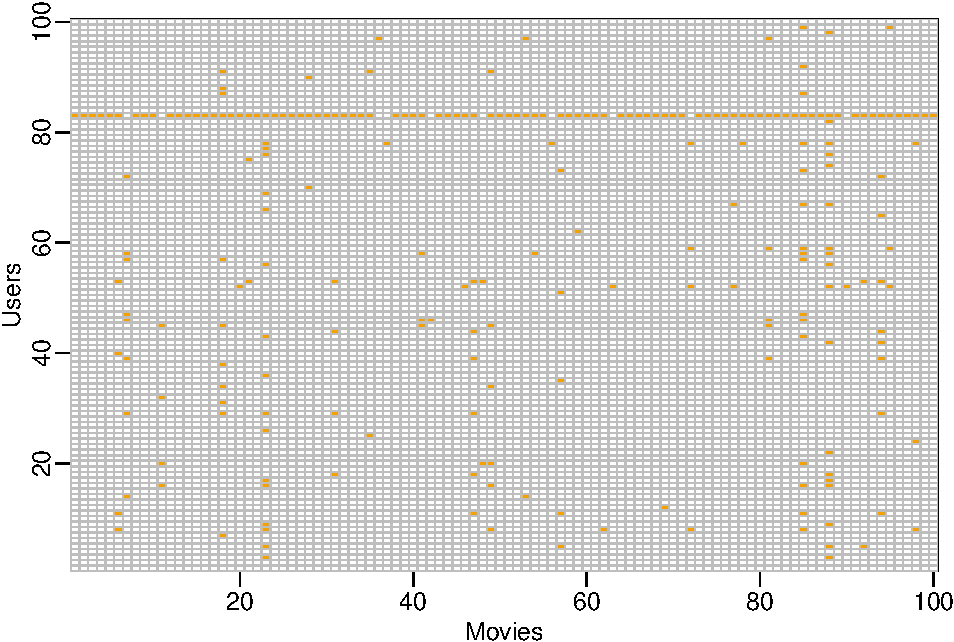
\includegraphics{figures/eda_4-1.pdf}
\caption{A Very Sparse Matrix\label{fig:matr}}
\end{figure}

This machine learning challenge is quite complicated, because each
outcome \(Y\) has a different set of predictors. To see this, note that
if we are predicting the rating for movie \emph{i} by user \emph{u}, in
principle, all other ratings related to movie \emph{i} and by user
\emph{u} may be used as predictors, but different users rate different
movies and a different number of movies. Furthermore, we may be able to
use information from other movies that we have determined are similar to
movie \emph{i} or from users determined to be similar to user \emph{u}.
In essence, the entire matrix can be used as predictors for each cell.

\newpage

\hypertarget{general-properties-of-the-data}{%
\paragraph{General Properties of the
data}\label{general-properties-of-the-data}}

Let's look at some of the \textbf{\emph{general properties}} of the data
to better understand the challenges.

The \textbf{\emph{first thing}} we notice is that some movies get rated
more than others. Figure \ref{fig:movies_getting_rated} shows the Movies
getting rated distribution. This should not surprise us given that there
are blockbuster movies watched by millions and artsy, independent movies
watched by just a few:

\begin{figure}
\centering
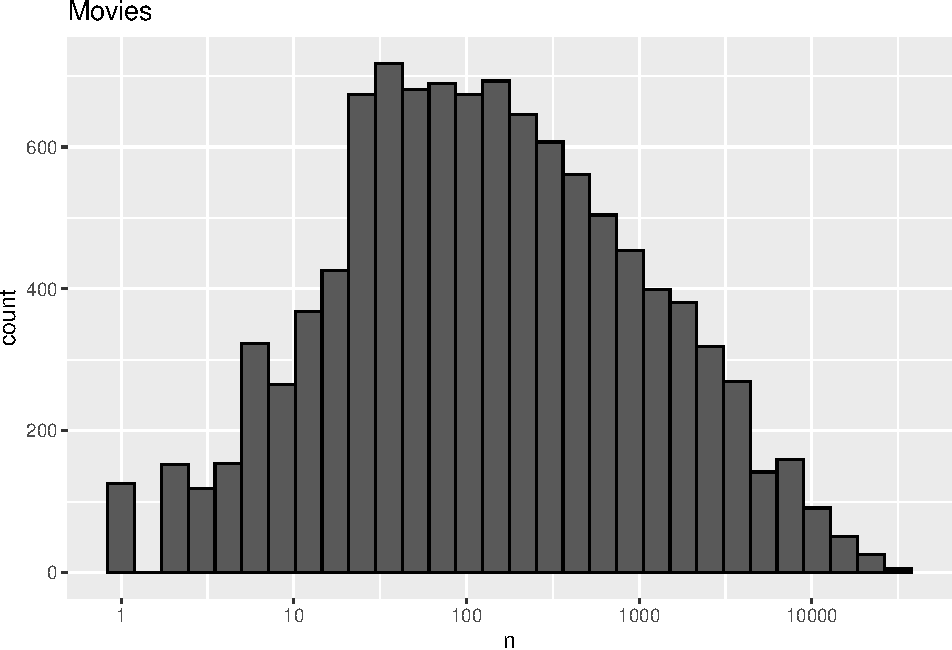
\includegraphics{figures/eda_5-1.pdf}
\caption{Movies getting rated
distribution\label{fig:movies_getting_rated}}
\end{figure}

\newpage

Our \textbf{\emph{second observation}} is that some users are more
active than others at rating movies. Figure
\ref{fig:users_rating_movies} shows Users rating movies distribution:

\begin{figure}
\centering
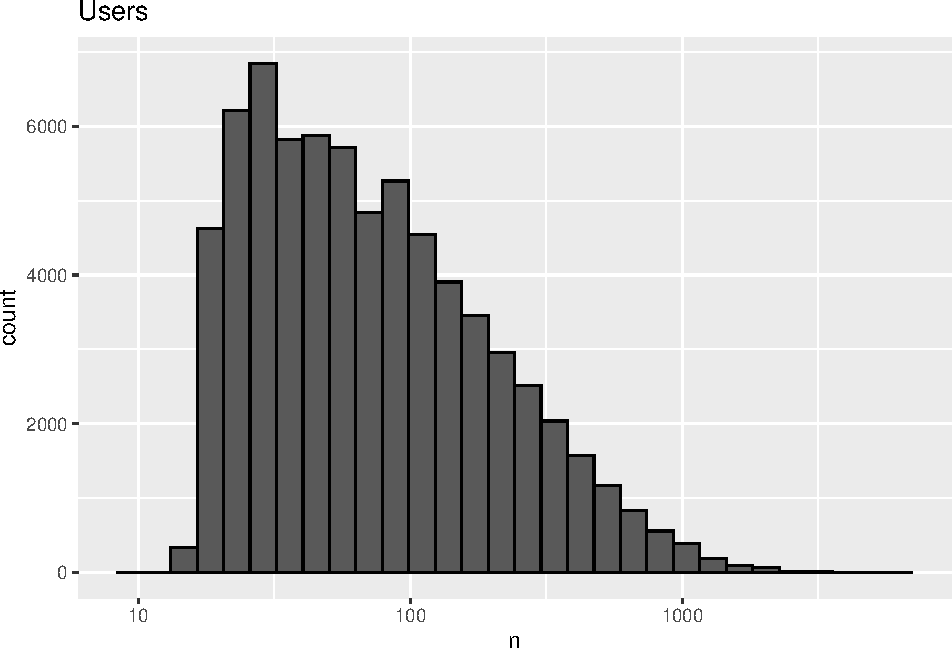
\includegraphics{figures/eda_6-1.pdf}
\caption{Users rating movies
distribution\label{fig:users_rating_movies}}
\end{figure}

\newpage

\hypertarget{further-data-exploration-visualization-modification}{%
\subsubsection{Further data Exploration, Visualization \&
Modification}\label{further-data-exploration-visualization-modification}}

\hypertarget{modify_edx}{%
\paragraph{Modify edx}\label{modify_edx}}

\textbf{Convert timestamp} in Movielens edx data Table
\ref{tbl:movielens_data} into date-time, a more readable and useful
format named \emph{rating\_date} in Table
\ref{tbl:movielens_edx_data_rating_date} below.

\begin{table}[H]

\caption{\label{tab:dw_1}Movielens edx data with rating date-time\label{tbl:movielens_edx_data_rating_date}}
\centering
\fontsize{8}{10}\selectfont
\begin{tabular}[t]{rrrlll}
\toprule
userId & movieId & rating & title & genres & rating\_date\\
\midrule
1 & 122 & 5 & Boomerang (1992) & Comedy|Romance & 1996-08-02 11:24:06\\
1 & 185 & 5 & Net, The (1995) & Action|Crime|Thriller & 1996-08-02 10:58:45\\
1 & 292 & 5 & Outbreak (1995) & Action|Drama|Sci-Fi|Thriller & 1996-08-02 10:57:01\\
1 & 316 & 5 & Stargate (1994) & Action|Adventure|Sci-Fi & 1996-08-02 10:56:32\\
1 & 329 & 5 & Star Trek: Generations (1994) & Action|Adventure|Drama|Sci-Fi & 1996-08-02 10:56:32\\
\bottomrule
\end{tabular}
\end{table}

\textbf{Split title} in Movielens edx data Table
\ref{tbl:movielens_data} into title and year movie released, a more
useful format named \emph{movie\_dt} in Table
\ref{tbl:movielens_edx_movie_release_date} below.

\begin{table}[H]

\caption{\label{tab:dw_2}Movielens edx data with movie release date\label{tbl:movielens_edx_movie_release_date}}
\centering
\fontsize{8}{10}\selectfont
\begin{tabular}[t]{rrrlllr}
\toprule
userId & movieId & rating & title & genres & rating\_date & movie\_dt\\
\midrule
1 & 122 & 5 & Boomerang & Comedy|Romance & 1996-08-02 11:24:06 & 1992\\
1 & 185 & 5 & Net, The & Action|Crime|Thriller & 1996-08-02 10:58:45 & 1995\\
1 & 292 & 5 & Outbreak & Action|Drama|Sci-Fi|Thriller & 1996-08-02 10:57:01 & 1995\\
1 & 316 & 5 & Stargate & Action|Adventure|Sci-Fi & 1996-08-02 10:56:32 & 1994\\
1 & 329 & 5 & Star Trek: Generations & Action|Adventure|Drama|Sci-Fi & 1996-08-02 10:56:32 & 1994\\
\bottomrule
\end{tabular}
\end{table}

\newpage

\hypertarget{modify-validation-repeat-above-steps}{%
\paragraph{Modify validation, repeat above
steps}\label{modify-validation-repeat-above-steps}}

\textbf{Convert timestamp} in Movielens validation data Table
\ref{tbl:movielens_data} into date-time, a more readable and useful
format named \emph{rating\_date} in Table
\ref{tbl:movielens_val_data_rating_date} below.

\begin{table}[H]

\caption{\label{tab:dw_3}Movielens validation data with rating date-time\label{tbl:movielens_val_data_rating_date}}
\centering
\fontsize{8}{10}\selectfont
\begin{tabular}[t]{rrrlll}
\toprule
userId & movieId & rating & title & genres & rating\_date\\
\midrule
1 & 231 & 5 & Dumb \& Dumber (1994) & Comedy & 1996-08-02 10:56:32\\
1 & 480 & 5 & Jurassic Park (1993) & Action|Adventure|Sci-Fi|Thriller & 1996-08-02 11:00:53\\
1 & 586 & 5 & Home Alone (1990) & Children|Comedy & 1996-08-02 11:07:48\\
2 & 151 & 3 & Rob Roy (1995) & Action|Drama|Romance|War & 1997-07-07 03:34:10\\
2 & 858 & 2 & Godfather, The (1972) & Crime|Drama & 1997-07-07 03:20:45\\
\bottomrule
\end{tabular}
\end{table}

\textbf{Split title} in Movielens validation data Table
\ref{tbl:movielens_data} into title and year movie released, a more
useful format named \emph{movie\_dt} in Table
\ref{tbl:movielens_val_movie_release_date} below.

\begin{table}[H]

\caption{\label{tab:dw_4}Movielens validation data with movie release date\label{tbl:movielens_val_movie_release_date}}
\centering
\fontsize{8}{10}\selectfont
\begin{tabular}[t]{rrrlllr}
\toprule
userId & movieId & rating & title & genres & rating\_date & movie\_dt\\
\midrule
1 & 231 & 5 & Dumb \& Dumber & Comedy & 1996-08-02 10:56:32 & 1994\\
1 & 480 & 5 & Jurassic Park & Action|Adventure|Sci-Fi|Thriller & 1996-08-02 11:00:53 & 1993\\
1 & 586 & 5 & Home Alone & Children|Comedy & 1996-08-02 11:07:48 & 1990\\
2 & 151 & 3 & Rob Roy & Action|Drama|Romance|War & 1997-07-07 03:34:10 & 1995\\
2 & 858 & 2 & Godfather, The & Crime|Drama & 1997-07-07 03:20:45 & 1972\\
\bottomrule
\end{tabular}
\end{table}

\newpage

\hypertarget{genres-combinations-per-movie---a-closer-look}{%
\paragraph{Genres combinations per movie - a closer
look}\label{genres-combinations-per-movie---a-closer-look}}

The movielens data Table \ref{tbl:movielens_edx_avg_rating_time_effect}
also has a genres column. This column includes every genre that applies
to the movie. Some movies fall under several genres. We define a
category of genres as whatever combination of genres appears in this
column, and refer to it as simply ``genres''.

Here we keep only categories with more than 1,000 ratings. Then compute
the average and standard error for each category, and plot these as
error bar plots. See Figure \ref{fig:genres_error_bar_plots} :

\begin{figure}
\centering
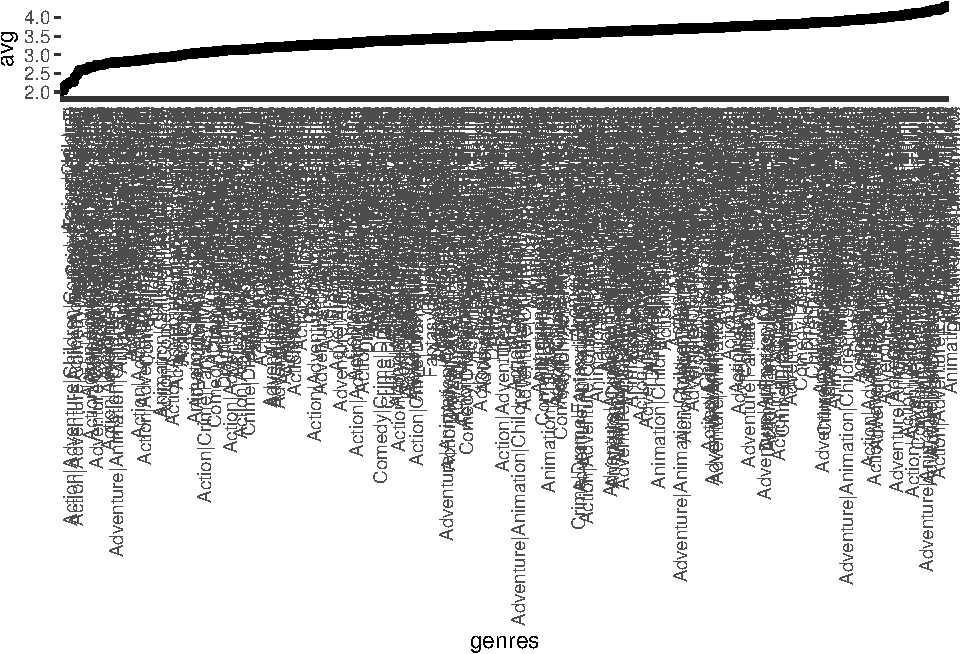
\includegraphics{figures/gnr-1.pdf}
\caption{Movies genres error bar
plots\label{fig:genres_error_bar_plots}}
\end{figure}

The plot shows strong evidence of a genre effect.

\newpage

\hypertarget{movie-rating-date-time---a-closer-look}{%
\paragraph{Movie Rating Date-Time - a closer
look}\label{movie-rating-date-time---a-closer-look}}

The Movielens edx data Table \ref{tbl:movielens_data} also includes a
time stamp. This variable represents the time and date in which the
rating was provided. The units are seconds since January 1, 1970. We
create a new column date with the date named \emph{rating\_date} in
subsection \protect\hyperlink{modify_edx}{Modify edx} to get Table
\ref{tbl:movielens_edx_movie_release_date} .

We compute the average rating for each week and plot this average
against day. See Figure
\ref{fig:movies_average_ratings_for_each_week_versus_day} :

\begin{verbatim}
`geom_smooth()` using method = 'loess' and formula 'y ~ x'
\end{verbatim}

\begin{figure}
\centering
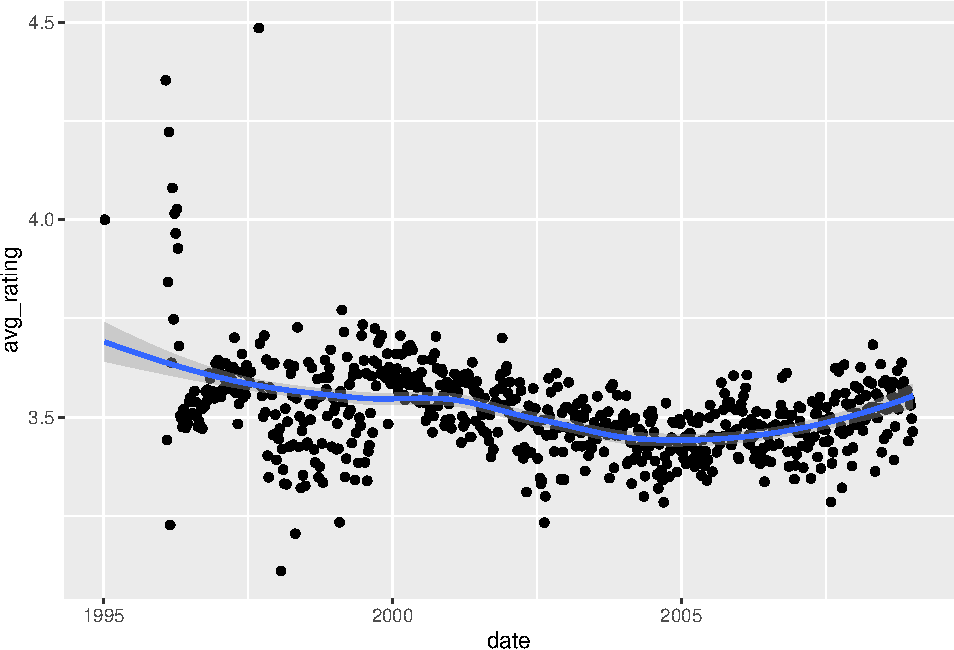
\includegraphics{figures/rd_1-1.pdf}
\caption{Movies average ratings for each week versus
day\label{fig:movies_average_ratings_for_each_week_versus_day}}
\end{figure}

The plot shows some evidence of a time effect. If we define \(d_{u,i}\)
as the day for user's \emph{u} rating of movie \emph{i}, then the
following model given by Equation \ref{eq:EqTimeEffect} is most
appropriate:

%
\refstepcounter{equations}
\addcontentsline{equ}{equations}{ \protect\numberline{\theequations}Movie Rating Date-Time effect Equation \ref{eq:EqTimeEffect}}\par

\label{eq:EqTimeEffect} \begin{equation}
Y_{u,i} = \mu + b_{i} + b_{u}  + f(d_{u,i})+ \epsilon_{u,i}\text{, with f a smooth function of }d_{u,i}
\end{equation}

\textbf{\emph{Modify edx}} Let's update the \textbf{\emph{edx}} table
with a new column for the average rating for each week and another
column for the day rounded to the nearest value of the week to get Table
\ref{tbl:movielens_edx_avg_rating_time_effect} below:

\begin{table}[H]

\caption{\label{tab:rd_2}Movielens edx data with average rating due to rating time effect\label{tbl:movielens_edx_avg_rating_time_effect}}
\centering
\fontsize{6}{8}\selectfont
\begin{tabular}[t]{rrrlllrlr}
\toprule
userId & movieId & rating & title & genres & rating\_date & movie\_dt & date & avg\_rating\\
\midrule
1 & 122 & 5 & Boomerang & Comedy|Romance & 1996-08-02 11:24:06 & 1992 & 1996-08-04 & 3.538801\\
1 & 185 & 5 & Net, The & Action|Crime|Thriller & 1996-08-02 10:58:45 & 1995 & 1996-08-04 & 3.538801\\
1 & 292 & 5 & Outbreak & Action|Drama|Sci-Fi|Thriller & 1996-08-02 10:57:01 & 1995 & 1996-08-04 & 3.538801\\
1 & 316 & 5 & Stargate & Action|Adventure|Sci-Fi & 1996-08-02 10:56:32 & 1994 & 1996-08-04 & 3.538801\\
1 & 329 & 5 & Star Trek: Generations & Action|Adventure|Drama|Sci-Fi & 1996-08-02 10:56:32 & 1994 & 1996-08-04 & 3.538801\\
\bottomrule
\end{tabular}
\end{table}

\textbf{TODO: Repeat above for validation data as well and somehow add
this to the modelling section}

\textbf{\emph{Modify validation}} We need to do the above
\textbf{\emph{avg\_rating\_time\_effect}} update for the validation data
as well. Let's update the \textbf{\emph{validation}} table to get Table
\ref{tbl:movielens_validation_avg_rating_time_effect} below:

\begin{table}[H]

\caption{\label{tab:rd_3}Movielens validation data with average rating due to rating time effect\label{tbl:movielens_validation_avg_rating_time_effect}}
\centering
\fontsize{6}{8}\selectfont
\begin{tabular}[t]{rrrlllrlr}
\toprule
userId & movieId & rating & title & genres & rating\_date & movie\_dt & date & avg\_rating\\
\midrule
1 & 231 & 5 & Dumb \& Dumber & Comedy & 1996-08-02 10:56:32 & 1994 & 1996-08-04 & 3.555820\\
1 & 480 & 5 & Jurassic Park & Action|Adventure|Sci-Fi|Thriller & 1996-08-02 11:00:53 & 1993 & 1996-08-04 & 3.555820\\
1 & 586 & 5 & Home Alone & Children|Comedy & 1996-08-02 11:07:48 & 1990 & 1996-08-04 & 3.555820\\
2 & 151 & 3 & Rob Roy & Action|Drama|Romance|War & 1997-07-07 03:34:10 & 1995 & 1997-07-06 & 3.606571\\
2 & 858 & 2 & Godfather, The & Crime|Drama & 1997-07-07 03:20:45 & 1972 & 1997-07-06 & 3.606571\\
\bottomrule
\end{tabular}
\end{table}

\newpage

\hypertarget{movie-release-date---a-closer-look}{%
\paragraph{Movie Release Date - a closer
look}\label{movie-release-date---a-closer-look}}

Computing the number of ratings for each movie and then plotting it
against the year the movie came out, that is the release date and using
the square root transformation on the counts using Table
\ref{tbl:movielens_edx_movie_release_date} , we get see Figure
\ref{fig:ratings_movie_release_date_all_dates} :

\textbf{TODO: Align images}

\begin{figure}[h!]

{\centering \subfloat[All data points only\label{fig:md_1-1}]{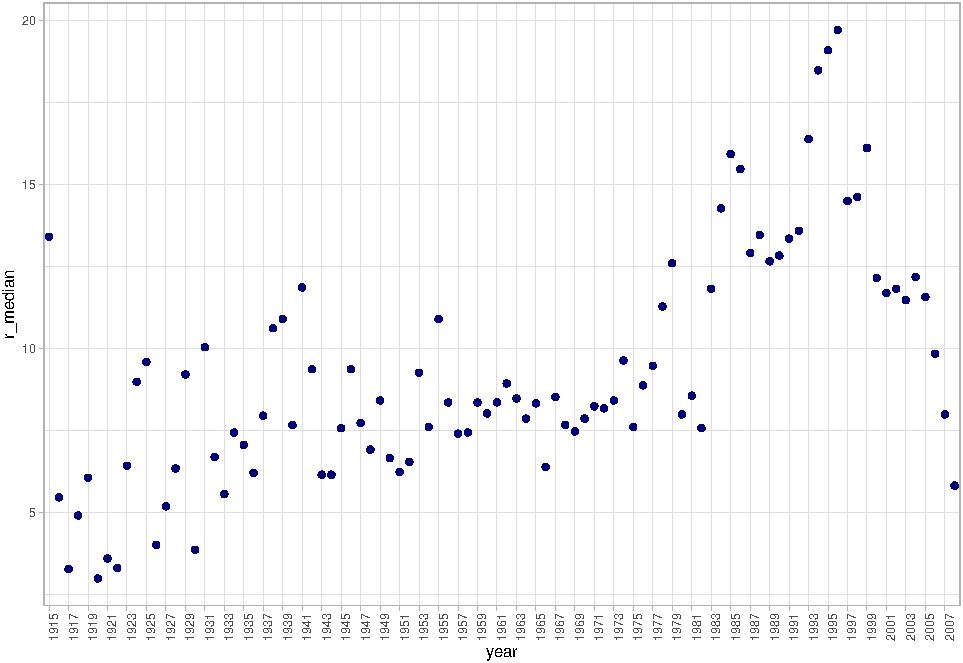
\includegraphics[width=0.7\linewidth]{figures/md_1-1} }\newline\subfloat[Smooth line through all data points\label{fig:md_1-2}]{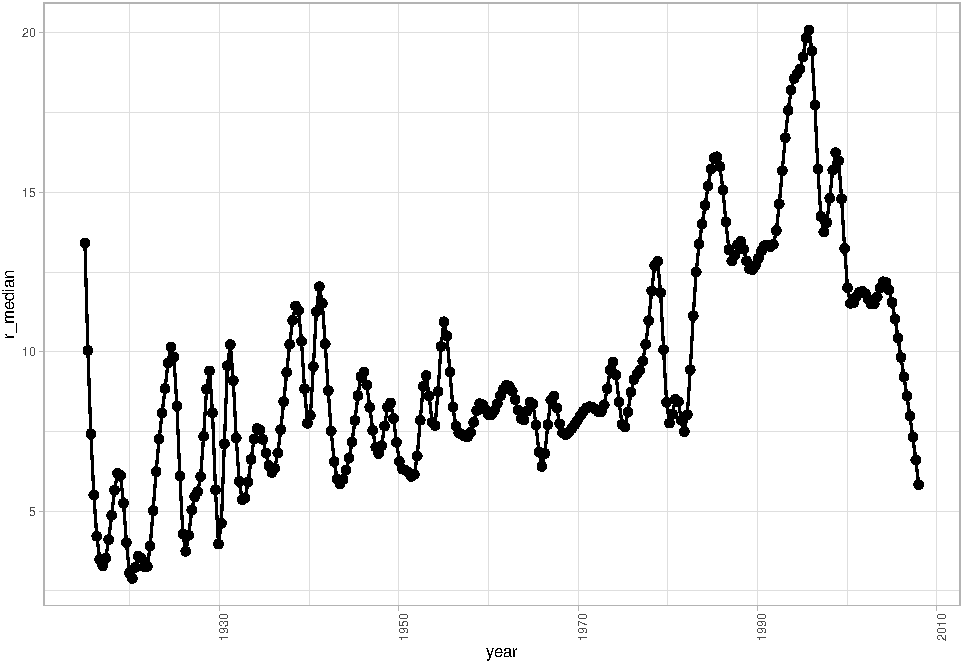
\includegraphics[width=0.7\linewidth]{figures/md_1-2} }

}

\caption{Ratings Movie Release Date - All dates\label{fig:ratings_movie_release_date_all_dates}}\label{fig:md_1}
\end{figure}

we see that, on average, movies that came out after 1993 get more
ratings. We also see that with newer movies, starting in 1993, the
number of ratings decreases with year: the more recent a movie is, the
less time users have had to rate it.

\newpage

Among movies that came out in 1993 or later, we select the top 25 movies
with the highest average number of ratings per year (n/year) and
calculate the average rating of each of them. To calculate number of
ratings per year, use 2018 as the end year. See Figure
\ref{fig:25_movies_avg_and_most_ratings_per_year_post_1993} :

\begin{verbatim}
`geom_smooth()` using method = 'loess' and formula 'y ~ x'
\end{verbatim}

\begin{figure}
\centering
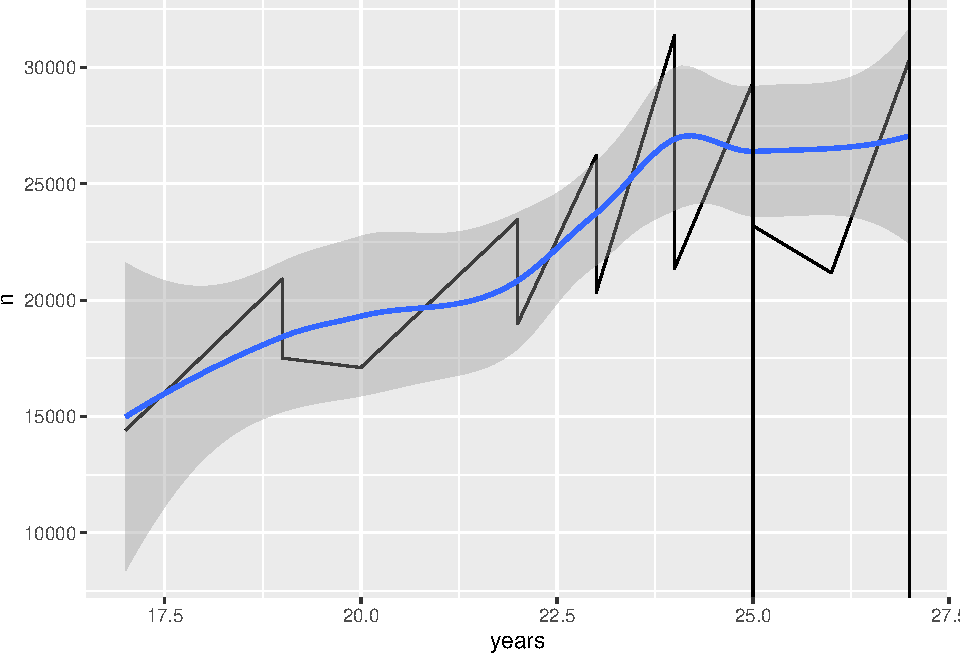
\includegraphics{figures/md_2-1.pdf}
\caption{25 Movies with the most ratings per year and their average
rating post
1993\label{fig:25_movies_avg_and_most_ratings_per_year_post_1993}}
\end{figure}

\newpage

We see that the most rated movies tend to have above average ratings.
This is not surprising: more people watch popular movies. To confirm
this, we stratify the post 1993 movies by ratings per year and compute
their average ratings. Figure
\ref{fig:movies_average_ratings_versus_ratings_per_year_post_1993} is a
plot of average ratings versus ratings per year showing an estimate of
the trend.

We see that the more a movie is rated, the higher the rating.

\textbf{Post-1993 movies}

\begin{verbatim}
`geom_smooth()` using method = 'gam' and formula 'y ~ s(x, bs = "cs")'
\end{verbatim}

\begin{figure}
\centering
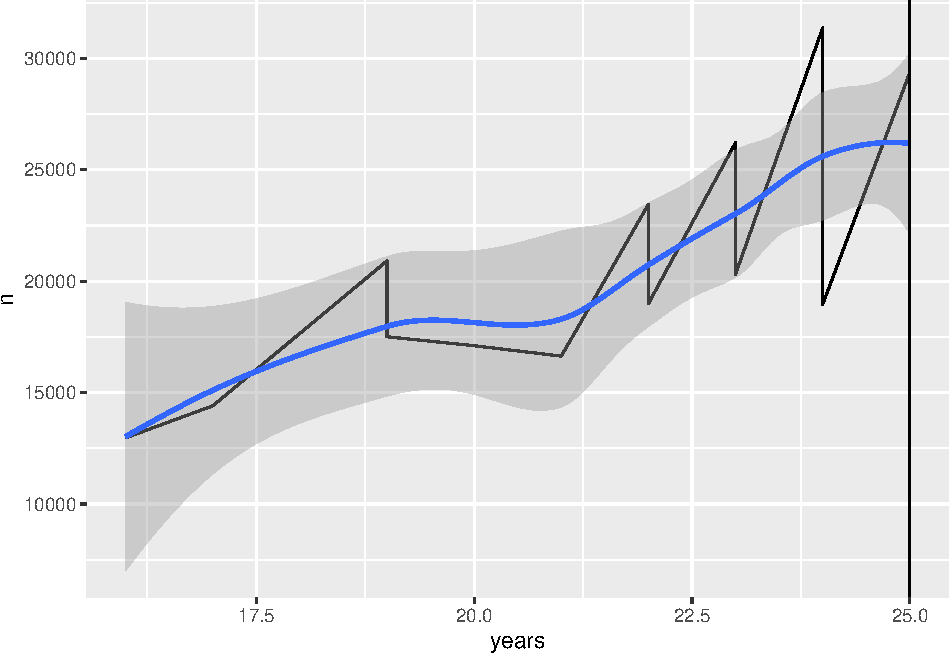
\includegraphics{figures/md_3-1.pdf}
\caption{Movies average ratings versus ratings per year post
1993\label{fig:movies_average_ratings_versus_ratings_per_year_post_1993}}
\end{figure}

\newpage

\textbf{Pre-1993 movies}\\
Compare Pre-1993 movies trend shown here in Figure
\ref{fig:movies_average_ratings_versus_ratings_per_year_pre_1993} Versus
Post-1993 movies trend in Figure
\ref{fig:movies_average_ratings_versus_ratings_per_year_post_1993}
above.

\begin{verbatim}
`geom_smooth()` using method = 'gam' and formula 'y ~ s(x, bs = "cs")'
\end{verbatim}

\begin{figure}
\centering
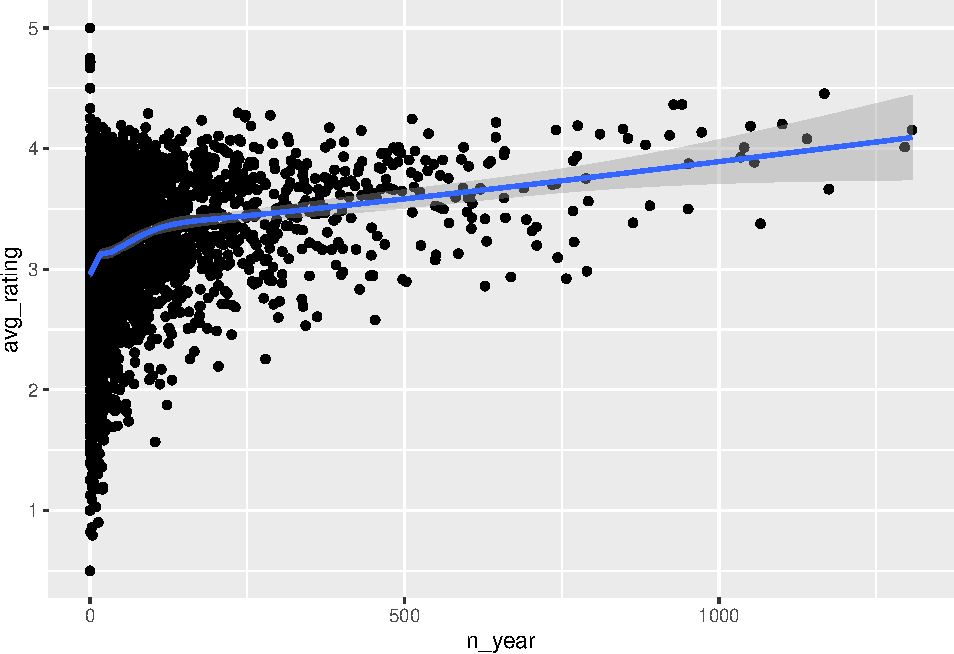
\includegraphics{figures/md_4-1.pdf}
\caption{Movies average ratings versus ratings per year pre
1993\label{fig:movies_average_ratings_versus_ratings_per_year_pre_1993}}
\end{figure}

\newpage

\textbf{\emph{Modify edx data for Release Date Effect}} We stratify the
movies by ratings per year and compute their average ratings based on
what we learnt above, where we confirmed our intuition that more people
watch popular movies. Finally edx data table looks as shown in Table
\ref{tbl:movielens_edx_avg_release_date_effect} below. Figure
\ref{fig:movies_average_ratings_versus_ratings_per_year_for_all_years_for_edx}
is a plot of average ratings versus ratings per year showing an estimate
of the trend.

\textbf{\emph{All Years}}

\begin{verbatim}
`geom_smooth()` using method = 'gam' and formula 'y ~ s(x, bs = "cs")'
\end{verbatim}

\begin{figure}
\centering
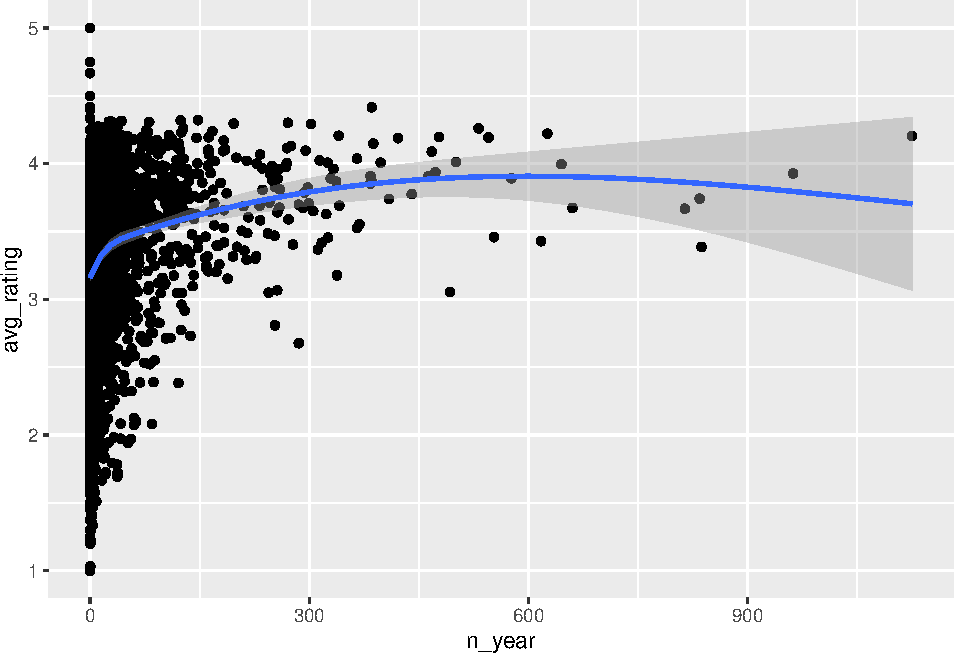
\includegraphics{figures/md_5-1.pdf}
\caption{Movies average ratings versus ratings per year for all years
for
edx\label{fig:movies_average_ratings_versus_ratings_per_year_for_all_years_for_edx}}
\end{figure}

\begin{table}[H]

\caption{\label{tab:md_6}Movielens edx data with average rating due to release date effect\label{tbl:movielens_edx_avg_release_date_effect}}
\centering
\fontsize{4}{6}\selectfont
\begin{tabular}[t]{rrrlllrlrrrrr}
\toprule
userId & movieId & rating & title & genres & rating\_date & movie\_dt & date & avg\_rating & avg\_rating\_rel & n & years & n\_year\\
\midrule
1 & 122 & 5 & Boomerang & Comedy|Romance & 1996-08-02 11:24:06 & 1992 & 1996-08-04 & 3.538801 & 2.858586 & 2178 & 26 & 84\\
1 & 185 & 5 & Net, The & Action|Crime|Thriller & 1996-08-02 10:58:45 & 1995 & 1996-08-04 & 3.538801 & 3.129334 & 13469 & 23 & 586\\
1 & 292 & 5 & Outbreak & Action|Drama|Sci-Fi|Thriller & 1996-08-02 10:57:01 & 1995 & 1996-08-04 & 3.538801 & 3.418011 & 14447 & 23 & 628\\
1 & 316 & 5 & Stargate & Action|Adventure|Sci-Fi & 1996-08-02 10:56:32 & 1994 & 1996-08-04 & 3.538801 & 3.349677 & 17030 & 24 & 710\\
1 & 329 & 5 & Star Trek: Generations & Action|Adventure|Drama|Sci-Fi & 1996-08-02 10:56:32 & 1994 & 1996-08-04 & 3.538801 & 3.337457 & 14550 & 24 & 606\\
\bottomrule
\end{tabular}
\end{table}

\begin{verbatim}
tibble [9,000,055 x 13] (S3: tbl_df/tbl/data.frame)
 $ userId        : int [1:9000055] 1 1 1 1 1 1 1 1 1 1 ...
 $ movieId       : num [1:9000055] 122 185 292 316 329 355 356 362 364 370 ...
 $ rating        : num [1:9000055] 5 5 5 5 5 5 5 5 5 5 ...
 $ title         : chr [1:9000055] "Boomerang " "Net, The " "Outbreak " "Stargate " ...
 $ genres        : chr [1:9000055] "Comedy|Romance" "Action|Crime|Thriller" "Action|Drama|Sci-Fi|Thriller" "Action|Adventure|Sci-Fi" ...
 $ rating_date   : POSIXct[1:9000055], format: "1996-08-02 11:24:06" "1996-08-02 10:58:45" ...
 $ movie_dt      : num [1:9000055] 1992 1995 1995 1994 1994 ...
 $ date          : POSIXct[1:9000055], format: "1996-08-04" "1996-08-04" ...
 $ avg_rating    : num [1:9000055] 3.54 3.54 3.54 3.54 3.54 ...
 $ avg_rating_rel: num [1:9000055] 2.86 3.13 3.42 3.35 3.34 ...
 $ n             : int [1:9000055] 2178 13469 14447 17030 14550 4831 31079 3612 18921 7331 ...
 $ years         : num [1:9000055] 26 23 23 24 24 24 24 24 24 24 ...
 $ n_year        : num [1:9000055] 84 586 628 710 606 ...
\end{verbatim}

\newpage

\textbf{\emph{Modify validation data for Release Date Effect}} We need
to do the above \textbf{\emph{avg\_rating\_rel\_effect}} update for the
validation data as well. Let's update the \textbf{\emph{validation}}
table to get Table
\ref{tbl:movielens_validation_avg_release_date_effect} below:

\textbf{\emph{All Years}}

\begin{table}[H]

\caption{\label{tab:md_7}Movielens validation data with average rating due to release date effect\label{tbl:movielens_validation_avg_release_date_effect}}
\centering
\fontsize{4}{6}\selectfont
\begin{tabular}[t]{rrrlllrlrrrrr}
\toprule
userId & movieId & rating & title & genres & rating\_date & movie\_dt & date & avg\_rating & avg\_rating\_rel & n & years & n\_year\\
\midrule
1 & 231 & 5 & Dumb \& Dumber & Comedy & 1996-08-02 10:56:32 & 1994 & 1996-08-04 & 3.555820 & 2.953281 & 1798 & 24 & 75\\
1 & 480 & 5 & Jurassic Park & Action|Adventure|Sci-Fi|Thriller & 1996-08-02 11:00:53 & 1993 & 1996-08-04 & 3.555820 & 3.643993 & 3271 & 25 & 131\\
1 & 586 & 5 & Home Alone & Children|Comedy & 1996-08-02 11:07:48 & 1990 & 1996-08-04 & 3.555820 & 3.074550 & 1556 & 28 & 56\\
2 & 151 & 3 & Rob Roy & Action|Drama|Romance|War & 1997-07-07 03:34:10 & 1995 & 1997-07-06 & 3.606571 & 3.571984 & 771 & 23 & 34\\
2 & 858 & 2 & Godfather, The & Crime|Drama & 1997-07-07 03:20:45 & 1972 & 1997-07-06 & 3.606571 & 4.412675 & 2067 & 46 & 45\\
\bottomrule
\end{tabular}
\end{table}

\begin{verbatim}
tibble [999,999 x 13] (S3: tbl_df/tbl/data.frame)
 $ userId        : int [1:999999] 1 1 1 2 2 2 3 3 4 4 ...
 $ movieId       : num [1:999999] 231 480 586 151 858 ...
 $ rating        : num [1:999999] 5 5 5 3 2 3 3.5 4.5 5 3 ...
 $ title         : chr [1:999999] "Dumb & Dumber " "Jurassic Park " "Home Alone " "Rob Roy " ...
 $ genres        : chr [1:999999] "Comedy" "Action|Adventure|Sci-Fi|Thriller" "Children|Comedy" "Action|Drama|Romance|War" ...
 $ rating_date   : POSIXct[1:999999], format: "1996-08-02 10:56:32" "1996-08-02 11:00:53" ...
 $ movie_dt      : num [1:999999] 1994 1993 1990 1995 1972 ...
 $ date          : POSIXct[1:999999], format: "1996-08-04" "1996-08-04" ...
 $ avg_rating    : num [1:999999] 3.56 3.56 3.56 3.61 3.61 ...
 $ avg_rating_rel: num [1:999999] 2.95 3.64 3.07 3.57 4.41 ...
 $ n             : int [1:999999] 1798 3271 1556 771 2067 862 2545 947 1869 776 ...
 $ years         : num [1:999999] 24 25 28 23 46 21 28 17 23 24 ...
 $ n_year        : num [1:999999] 75 131 56 34 45 41 91 56 81 32 ...
\end{verbatim}

\newpage

\hypertarget{analysis---model-building-and-evaluation}{%
\section{Analysis - Model Building and
Evaluation}\label{analysis---model-building-and-evaluation}}

\hypertarget{split-the-edx-data-into-separate-training-and-test-sets}{%
\subsection{Split the edx data into separate training and test
sets}\label{split-the-edx-data-into-separate-training-and-test-sets}}

We will develop our algorithm using the edx set only.\\
We will split the edx data into separate training and test sets to
design and test our algorithm, namely train\_set and test\_set.

\hypertarget{loss-function}{%
\subsubsection{Loss function}\label{loss-function}}

For a final test of our algorithm, we predict movie ratings in the test
set as if they were unknown.
\href{https://en.wikipedia.org/wiki/Root-mean-square_deviation}{RMSE}
(residual mean squared error/root mean square error), the typical error
loss, will be used to evaluate how close our predictions are to the true
values in the validation set.\\
We define \({y_{u,i}}\) as the rating for movie \emph{i} by user
\emph{u} and denote our prediction with \({\hat{y}_{u,i}}\).

The RMSE is then defined as Equation \ref{eq:EqLossFunction}:

%
\refstepcounter{equations}
\addcontentsline{equ}{equations}{ \protect\numberline{\theequations}Loss function RMSE Equation \ref{eq:EqLossFunction}}\par

\label{eq:EqLossFunction} \begin{equation}
  RMSE=\sqrt{\frac{1}{N}\sum_{u,i}(\hat{y}_{u,i}-y_{u,i})^{2}}
\end{equation}

with N being the number of user/movie combinations and the sum occurring
over all these combinations.

Remember that we can interpret the RMSE similarly to a standard
deviation: it is the typical error we make when predicting a movie
rating. If this number is larger than 1, it means our typical error is
larger than one star, which is not good.

Let's write a function that computes the RMSE for vectors of ratings and
their corresponding predictors:

\begin{Shaded}
\begin{Highlighting}[]
\NormalTok{RMSE }\OtherTok{\textless{}{-}} \ControlFlowTok{function}\NormalTok{(true\_ratings, predicted\_ratings) \{}
    \FunctionTok{sqrt}\NormalTok{(}\FunctionTok{mean}\NormalTok{((true\_ratings }\SpecialCharTok{{-}}\NormalTok{ predicted\_ratings)}\SpecialCharTok{\^{}}\DecValTok{2}\NormalTok{))}
\NormalTok{\}}
\end{Highlighting}
\end{Shaded}

\newpage

\hypertarget{model-1-a-first-naive-mean-model}{%
\subsection{Model 1: A first naive ``mean''
model}\label{model-1-a-first-naive-mean-model}}

Let's start by building the simplest possible recommendation system: we
predict the same rating for all movies regardless of user. A model that
assumes the same rating for all movies and users with all the
differences explained by random variation would look like Equation
\ref{eq:EqModel1}:

%
\refstepcounter{equations}
\addcontentsline{equ}{equations}{ \protect\numberline{\theequations}Model 1: A naive "mean" model Equation \ref{eq:EqModel1}}\par

\label{eq:EqModel1} \begin{equation}
  Y_{i,i} = \mu + \epsilon_{u,i}
\end{equation}

with \(\epsilon_{u,i}\) independent errors sampled from the same
distribution centered at 0 and \(\mu\) the ``true'' rating for all
movies. We know that the estimate that minimizes the RMSE is the least
squares estimate of \(\mu\) and, in this case, is the average of all
ratings:

\begin{Shaded}
\begin{Highlighting}[]
\NormalTok{(mu\_hat }\OtherTok{\textless{}{-}} \FunctionTok{mean}\NormalTok{(train\_set}\SpecialCharTok{$}\NormalTok{rating))}
\NormalTok{[}\DecValTok{1}\NormalTok{] }\FloatTok{3.512482}
\end{Highlighting}
\end{Shaded}

If we predict all unknown ratings with \(\hat\mu\) we obtain the
following RMSE:

\begin{Shaded}
\begin{Highlighting}[]
\NormalTok{(model\_1\_rmse }\OtherTok{\textless{}{-}} \FunctionTok{RMSE}\NormalTok{(test\_set}\SpecialCharTok{$}\NormalTok{rating, mu\_hat))}
\NormalTok{[}\DecValTok{1}\NormalTok{] }\FloatTok{1.059904}
\end{Highlighting}
\end{Shaded}

Keep in mind that if we plug in any other number, we get a higher RMSE.
For example:

\begin{Shaded}
\begin{Highlighting}[]
\NormalTok{predictions }\OtherTok{\textless{}{-}} \FunctionTok{rep}\NormalTok{(}\FloatTok{2.5}\NormalTok{, }\FunctionTok{nrow}\NormalTok{(test\_set))}
\FunctionTok{RMSE}\NormalTok{(test\_set}\SpecialCharTok{$}\NormalTok{rating, predictions)}
\NormalTok{[}\DecValTok{1}\NormalTok{] }\FloatTok{1.465736}

\NormalTok{predictions }\OtherTok{\textless{}{-}} \FunctionTok{rep}\NormalTok{(}\DecValTok{3}\NormalTok{, }\FunctionTok{nrow}\NormalTok{(test\_set))}
\FunctionTok{RMSE}\NormalTok{(test\_set}\SpecialCharTok{$}\NormalTok{rating, predictions)}
\NormalTok{[}\DecValTok{1}\NormalTok{] }\FloatTok{1.177271}

\NormalTok{predictions }\OtherTok{\textless{}{-}} \FunctionTok{rep}\NormalTok{(}\DecValTok{4}\NormalTok{, }\FunctionTok{nrow}\NormalTok{(test\_set))}
\FunctionTok{RMSE}\NormalTok{(test\_set}\SpecialCharTok{$}\NormalTok{rating, predictions)}
\NormalTok{[}\DecValTok{1}\NormalTok{] }\FloatTok{1.166678}
\end{Highlighting}
\end{Shaded}

From looking at the distribution of ratings, we can visualize that this
is the standard deviation of that distribution. We get a RMSE of about
1. Our target is RMSE \textless{} 0.86490. So we can definitely do
better!

\newpage

\hypertarget{results-model-1}{%
\subsubsection{Results Model 1}\label{results-model-1}}

As we go along, we will be comparing different approaches. Let's start
by creating a results table with this naive approach to get Table
\ref{tbl:rmse_results_model_1}:

\begin{table}[H]

\caption{\label{tab:m_1_4}RMSE Results Model 1\label{tbl:rmse_results_model_1}}
\centering
\fontsize{7}{9}\selectfont
\begin{tabular}[t]{llr}
\toprule
Index & Method & RMSE\\
\midrule
1 & Just the average & 1.059904\\
\bottomrule
\end{tabular}
\end{table}

\newpage

\hypertarget{model-2-movie-effects}{%
\subsection{Model 2: Movie effects}\label{model-2-movie-effects}}

We know from experience that some movies are just generally rated higher
than others. This intuition, that different movies are rated
differently, is confirmed by data. We can augment our previous model by
adding the term \(b_{i}\) to represent average ranking for movie
\emph{i} and would look like Equation \ref{eq:EqModel2-1}:

%
\refstepcounter{equations}
\addcontentsline{equ}{equations}{ \protect\numberline{\theequations}Model 2: Movie effects linear model Equation \ref{eq:EqModel2-1}}\par

\label{eq:EqModel2-1} \begin{equation}
  Y_{u,i} = \mu + b_{i} + \epsilon_{u,i}
\end{equation}

Statistics textbooks refer to the \emph{b}s as effects or
\emph{``bias''}.

We can again use least squares to estimate the \(b_{i}\) in the
following way to get Equation \ref{eq:EqModel2-2}:

%
\refstepcounter{equations}
\addcontentsline{equ}{equations}{ \protect\numberline{\theequations}LSE linear function to fit Movie effects linear model Equation \ref{eq:EqModel2-2}}\par

\label{eq:EqModel2-2} \begin{equation}
  fit \leftarrow lm(rating \; \sim \; as.factor(userId), \: data = train\_{}set)
\end{equation}

Because there are thousands of \(b_{i}\) as each movie gets one, the
lm() function will be very slow here. We therefore will not run the code
above.

But in this particular situation, we know that the least squares
estimate \(\hat{b_{i}}\) is just the average of \(Y_{u,i}-\hat{\mu}\)
for each movie \emph{i}. \textbf{\emph{So we can compute them this way
(we will drop the hat notation in the code to represent estimates going
forward)}}:

%
\refstepcounter{equations}
\addcontentsline{equ}{equations}{ \protect\numberline{\theequations}Movie specific effects Equation \ref{eq:EqModel2-3}}\par

\label{eq:EqModel2-3} \begin{equation}
  \hat{b_{i}} = \overline{y_{u,i} - \hat{\mu}}
\end{equation}

\begin{Shaded}
\begin{Highlighting}[]
\NormalTok{mu }\OtherTok{\textless{}{-}} \FunctionTok{mean}\NormalTok{(train\_set}\SpecialCharTok{$}\NormalTok{rating)}
\end{Highlighting}
\end{Shaded}

\newpage

We can see that these estimates vary substantially, see Figure
\ref{fig:model_2}

\begin{figure}
\centering
\includegraphics{figures/me_2-1.pdf}
\caption{Movie effect or bias distribution\label{fig:model_2}}
\end{figure}

Remember \(\hat{\mu}\)=3.5 so a \(b_{i}\)=1.5 implies a perfect five
star rating. Let's see how much our prediction improves once we use
\(\hat{y_{u,i}}=\hat{\mu}+\hat{b_{i}}\):

\begin{Shaded}
\begin{Highlighting}[]
\NormalTok{predicted\_ratings\_model\_2 }\OtherTok{\textless{}{-}}\NormalTok{ mu }\SpecialCharTok{+}\NormalTok{ test\_set }\SpecialCharTok{\%\textgreater{}\%} 
  \FunctionTok{left\_join}\NormalTok{(movie\_avgs, }\AttributeTok{by=}\StringTok{\textquotesingle{}movieId\textquotesingle{}}\NormalTok{) }\SpecialCharTok{\%\textgreater{}\%} 
\NormalTok{  .}\SpecialCharTok{$}\NormalTok{b\_i}

\NormalTok{[}\DecValTok{1}\NormalTok{] }\FloatTok{0.9437429}
\end{Highlighting}
\end{Shaded}

\newpage

\hypertarget{results-model-1-2}{%
\subsubsection{Results Model 1-2}\label{results-model-1-2}}

Let's add the movie effects model to our results table to get Table
\ref{tbl:rmse_results_model_1-2}

\begin{table}[H]

\caption{\label{tab:me_4}RMSE Results Models 1-2\label{tbl:rmse_results_model_1-2}}
\centering
\fontsize{7}{9}\selectfont
\begin{tabular}[t]{llr}
\toprule
Index & Method & RMSE\\
\midrule
1 & Just the average & 1.0599043\\
2 & Movie Effect Model & 0.9437429\\
\bottomrule
\end{tabular}
\end{table}

\newpage

\hypertarget{model-3-user-effects}{%
\subsection{Model 3: User effects}\label{model-3-user-effects}}

Let's compute \emph{b\_u} the average rating for user \emph{u} for those
that have rated over 100 movies, see Figure
\ref{fig:average_ratings_for_users_who_have_rated_over_100_movies}

\begin{Shaded}
\begin{Highlighting}[]
\NormalTok{train\_set }\SpecialCharTok{\%\textgreater{}\%} 
  \FunctionTok{group\_by}\NormalTok{(userId) }\SpecialCharTok{\%\textgreater{}\%} 
  \FunctionTok{summarize}\NormalTok{(}\AttributeTok{b\_u =} \FunctionTok{mean}\NormalTok{(rating)) }\SpecialCharTok{\%\textgreater{}\%} 
  \FunctionTok{filter}\NormalTok{(}\FunctionTok{n}\NormalTok{()}\SpecialCharTok{\textgreater{}=}\DecValTok{100}\NormalTok{) }\SpecialCharTok{\%\textgreater{}\%}
  \FunctionTok{ggplot}\NormalTok{(}\FunctionTok{aes}\NormalTok{(b\_u)) }\SpecialCharTok{+} 
  \FunctionTok{geom\_histogram}\NormalTok{(}\AttributeTok{bins =} \DecValTok{30}\NormalTok{, }\AttributeTok{color =} \StringTok{"black"}\NormalTok{) }\SpecialCharTok{+} 
  \FunctionTok{ggtitle}\NormalTok{(}\StringTok{"Average rating for users who have rated over 100 movies"}\NormalTok{)}
\end{Highlighting}
\end{Shaded}

\begin{figure}
\centering
\includegraphics{figures/ue_1-1.pdf}
\caption{Average rating for users who have rated over 100
movies\label{fig:average_ratings_for_users_who_have_rated_over_100_movies}}
\end{figure}

\newpage

Let's compute \emph{b\_u} the average rating for user \emph{u} for those
that have rated any movies, see Figure
\ref{fig:average_ratings_for_users_who_have_rated_any_movies}

\begin{Shaded}
\begin{Highlighting}[]
\NormalTok{train\_set }\SpecialCharTok{\%\textgreater{}\%} 
  \FunctionTok{group\_by}\NormalTok{(userId) }\SpecialCharTok{\%\textgreater{}\%} 
  \FunctionTok{summarize}\NormalTok{(}\AttributeTok{b\_u =} \FunctionTok{mean}\NormalTok{(rating)) }\SpecialCharTok{\%\textgreater{}\%} 
  \FunctionTok{ggplot}\NormalTok{(}\FunctionTok{aes}\NormalTok{(b\_u)) }\SpecialCharTok{+} 
  \FunctionTok{geom\_histogram}\NormalTok{(}\AttributeTok{bins =} \DecValTok{30}\NormalTok{, }\AttributeTok{color =} \StringTok{"black"}\NormalTok{) }\SpecialCharTok{+} 
  \FunctionTok{ggtitle}\NormalTok{(}\StringTok{"Average rating for users who have rated any movies"}\NormalTok{)}
\end{Highlighting}
\end{Shaded}

\begin{figure}
\centering
\includegraphics{figures/ue_2-1.pdf}
\caption{Average rating for users who have rated any
movies\label{fig:average_ratings_for_users_who_have_rated_any_movies}}
\end{figure}

Notice that there is substantial variability across users as well: some
users are very cranky and others love every movie. This implies that a
further improvement to our model may be as shown in Equation
\ref{eq:EqModel3-1}:

%
\refstepcounter{equations}
\addcontentsline{equ}{equations}{ \protect\numberline{\theequations}Model 3: Movie + User effects linear model Equation \ref{eq:EqModel3-1}}\par

\label{eq:EqModel3-1} \begin{equation}
  Y_{u,i} = \mu + b_{i} + b_{u} + \epsilon_{u,i}
\end{equation}

where \(b_{u}\) is a user-specific effect. Now if a cranky user
(negative \(b_{u}\)) rates a great movie (positive \(b_{i}\)), the
effects counter each other and we may be able to correctly predict that
this user gave this great movie a 3 rather than a 5.

To fit this model, we could again use lm() as shown in Equation
\ref{eq:EqModel3-2}:

%
\refstepcounter{equations}
\addcontentsline{equ}{equations}{ \protect\numberline{\theequations}LSE linear function to fit Movie + User effects linear model Equation \ref{eq:EqModel3-2}}\par

\label{eq:EqModel3-2} \begin{equation}
  fit \leftarrow lm(rating \; \sim \; as.factor(movieId) + as.factor(userId), \: data = train\_{}set)
\end{equation}

but, for the reasons described earlier, we won't. Instead, we will
compute an approximation by computing \(\hat{\mu}\) and \(\hat{b_{i}}\)
and estimating \(\hat{b_{u}}\) as the average of
\(y_{u,i}-\hat{\mu}-\hat{b_{i}}\):

%
\refstepcounter{equations}
\addcontentsline{equ}{equations}{ \protect\numberline{\theequations}User specific effects Equation \ref{eq:EqModel3-3}}\par

\label{eq:EqModel3-3} \begin{equation}
  \hat{b_{u}} = \overline{y_{u,i} - \hat{\mu} - \hat{b_{i}}}
\end{equation}

\newpage

\begin{Shaded}
\begin{Highlighting}[]
\NormalTok{user\_avgs }\OtherTok{\textless{}{-}}\NormalTok{ train\_set }\SpecialCharTok{\%\textgreater{}\%} 
  \FunctionTok{left\_join}\NormalTok{(movie\_avgs, }\AttributeTok{by=}\StringTok{\textquotesingle{}movieId\textquotesingle{}}\NormalTok{) }\SpecialCharTok{\%\textgreater{}\%}
  \FunctionTok{group\_by}\NormalTok{(userId) }\SpecialCharTok{\%\textgreater{}\%}
  \FunctionTok{summarize}\NormalTok{(}\AttributeTok{b\_u =} \FunctionTok{mean}\NormalTok{(rating }\SpecialCharTok{{-}}\NormalTok{ mu }\SpecialCharTok{{-}}\NormalTok{ b\_i))}
\end{Highlighting}
\end{Shaded}

We can see that these estimates vary substantially, see Figure
\ref{fig:model_3}

\begin{figure}
\centering
\includegraphics{figures/ue_4-1.pdf}
\caption{User effect or bias distribution\label{fig:model_3}}
\end{figure}

We can now construct predictors and see how much the RMSE improves:

\begin{Shaded}
\begin{Highlighting}[]
\NormalTok{predicted\_ratings\_model\_3 }\OtherTok{\textless{}{-}}\NormalTok{ test\_set }\SpecialCharTok{\%\textgreater{}\%} 
  \FunctionTok{left\_join}\NormalTok{(movie\_avgs, }\AttributeTok{by=}\StringTok{\textquotesingle{}movieId\textquotesingle{}}\NormalTok{) }\SpecialCharTok{\%\textgreater{}\%}
  \FunctionTok{left\_join}\NormalTok{(user\_avgs, }\AttributeTok{by=}\StringTok{\textquotesingle{}userId\textquotesingle{}}\NormalTok{) }\SpecialCharTok{\%\textgreater{}\%}
  \FunctionTok{mutate}\NormalTok{(}\AttributeTok{pred =}\NormalTok{ mu }\SpecialCharTok{+}\NormalTok{ b\_i }\SpecialCharTok{+}\NormalTok{ b\_u) }\SpecialCharTok{\%\textgreater{}\%}
\NormalTok{  .}\SpecialCharTok{$}\NormalTok{pred}

\NormalTok{[}\DecValTok{1}\NormalTok{] }\FloatTok{0.865932}
\end{Highlighting}
\end{Shaded}

\newpage

\hypertarget{results-table-model-1-3}{%
\subsubsection{Results Table Model 1-3}\label{results-table-model-1-3}}

Let's add the user effects model to our results table to get Table
\ref{tbl:rmse_results_model_1-3}

\begin{table}[H]

\caption{\label{tab:ue_6}RMSE Results Models 1-3\label{tbl:rmse_results_model_1-3}}
\centering
\fontsize{7}{9}\selectfont
\begin{tabular}[t]{llr}
\toprule
Index & Method & RMSE\\
\midrule
1 & Just the average & 1.0599043\\
2 & Movie Effect Model & 0.9437429\\
3 & Movie + User Effects Model & 0.8659320\\
\bottomrule
\end{tabular}
\end{table}

\newpage

\hypertarget{model-4-genre-effects}{%
\subsection{Model 4: Genre effects}\label{model-4-genre-effects}}

The movielens data also has a genres column. This column includes every
genre that applies to the movie. Some movies fall under several genres.
Define a category of genres as whatever combination of genres appears in
this column. We will refer to this category as simply ``genres''.

There is strong evidence of a genre effect as we have shown earlier in
Figure \ref{fig:genres_error_bar_plots}, and in this section below in
Figure \ref{fig:model_4}. If we define \(g_{u,i}\) as the genre for
\emph{u} user's rating of movie \emph{i}, then the following model as
shown in Equation \ref{eq:EqModel4-1} is most appropriate:

%
\refstepcounter{equations}
\addcontentsline{equ}{equations}{ \protect\numberline{\theequations}Model 4: Movie + User + Genre effects linear model Equation \ref{eq:EqModel4-1}}\par

\label{eq:EqModel4-1} \begin{equation}
  Y_{u,i} = \mu + b_{i} + b_{u} + \sum_{k=1}^Kx_{u,i}\beta_k + \epsilon_{u,i}
\end{equation}

\begin{center}
with $x_{u,i}^k=1$ if $g_{u,i}$ is genre *k*
\end{center}

\begin{Shaded}
\begin{Highlighting}[]
\NormalTok{train\_set }\SpecialCharTok{\%\textgreater{}\%} 
  \FunctionTok{group\_by}\NormalTok{(genres) }\SpecialCharTok{\%\textgreater{}\%} 
  \FunctionTok{summarize}\NormalTok{(}\AttributeTok{mu\_g =} \FunctionTok{mean}\NormalTok{(rating)) }\SpecialCharTok{\%\textgreater{}\%} 
  \FunctionTok{ggplot}\NormalTok{(}\FunctionTok{aes}\NormalTok{(mu\_g)) }\SpecialCharTok{+} 
  \FunctionTok{geom\_histogram}\NormalTok{(}\AttributeTok{bins =} \DecValTok{30}\NormalTok{, }\AttributeTok{color =} \StringTok{"black"}\NormalTok{) }\SpecialCharTok{+} 
  \FunctionTok{ggtitle}\NormalTok{(}\StringTok{"Average rating for movies of category genres"}\NormalTok{)}
\end{Highlighting}
\end{Shaded}

\begin{figure}
\centering
\includegraphics{figures/ge_1-1.pdf}
\caption{Average rating for movies of category
genres\label{fig:average_ratings_for_movies_of_category_genres}}
\end{figure}

To fit this model, we could again use the lm() function as shown in
Equation \ref{eq:EqModel4-2}:

%
\refstepcounter{equations}
\addcontentsline{equ}{equations}{ \protect\numberline{\theequations}LSE linear function to fit Movie + User + Genres effects linear model Equation \ref{eq:EqModel4-2}}\par

\label{eq:EqModel4-2} \begin{equation}
\begin{split}
  fit \leftarrow lm(rating \; \sim \; & as.factor(movieId) + as.factor(userId) + \\ 
  & as.factor(genres), \: data = train\_{}set)
\end{split}
\end{equation}

but, for the reasons described earlier, we won't. Instead, we will
compute an approximation by computing \(\hat{\mu}\), \(\hat{b_{i}}\),
\(\hat{b_{u}}\) and estimating \(\hat{b_{g}}\) as the average of
\(y_{u,i}-\hat{\mu}-\hat{b_{i}}-\hat{b_{u}}\) :

%
\refstepcounter{equations}
\addcontentsline{equ}{equations}{ \protect\numberline{\theequations}Genres specific effects Equation \ref{eq:EqModel4-3}}\par

\label{eq:EqModel4-3} \begin{equation}
  \hat{b_{g}} = \overline{y_{u,i} - \hat{\mu} - \hat{b_{i}} - \hat{b_{u}}}
\end{equation}

where:

%
\refstepcounter{equations}
\addcontentsline{equ}{equations}{ \protect\numberline{\theequations}Genres specific effects Equation \ref{eq:EqModel4-4}}\par

\label{eq:EqModel4-4} \begin{equation}
  \hat{b_{g}} = \sum_{k=1}^Kx_{u,i}\beta_k
\end{equation}

\begin{center}
with $x_{u,i}^k=1$ if $g_{u,i}$ is genre *k*
\end{center}

where \(\hat{b_{g}}\) is genre specific effect.

\begin{Shaded}
\begin{Highlighting}[]
\NormalTok{genres\_avgs }\OtherTok{\textless{}{-}}\NormalTok{ train\_set }\SpecialCharTok{\%\textgreater{}\%} 
  \FunctionTok{left\_join}\NormalTok{(movie\_avgs, }\AttributeTok{by=}\StringTok{\textquotesingle{}movieId\textquotesingle{}}\NormalTok{) }\SpecialCharTok{\%\textgreater{}\%} 
  \FunctionTok{left\_join}\NormalTok{(user\_avgs, }\AttributeTok{by=}\StringTok{\textquotesingle{}userId\textquotesingle{}}\NormalTok{) }\SpecialCharTok{\%\textgreater{}\%}
  \FunctionTok{group\_by}\NormalTok{(genres) }\SpecialCharTok{\%\textgreater{}\%}
  \FunctionTok{summarize}\NormalTok{(}\AttributeTok{b\_g =} \FunctionTok{mean}\NormalTok{(rating }\SpecialCharTok{{-}}\NormalTok{ mu }\SpecialCharTok{{-}}\NormalTok{ b\_i }\SpecialCharTok{{-}}\NormalTok{ b\_u))}
\end{Highlighting}
\end{Shaded}

We can see that these estimates vary substantially, see Figure
\ref{fig:model_4}

\begin{figure}
\centering
\includegraphics{figures/ge_4-1.pdf}
\caption{Genres effect or bias distribution\label{fig:model_4}}
\end{figure}

We can now construct predictors and see how much the RMSE improves:

\begin{Shaded}
\begin{Highlighting}[]
\NormalTok{predicted\_ratings\_model\_4 }\OtherTok{\textless{}{-}}\NormalTok{ test\_set }\SpecialCharTok{\%\textgreater{}\%} 
  \FunctionTok{left\_join}\NormalTok{(movie\_avgs, }\AttributeTok{by=}\StringTok{\textquotesingle{}movieId\textquotesingle{}}\NormalTok{) }\SpecialCharTok{\%\textgreater{}\%} 
  \FunctionTok{left\_join}\NormalTok{(user\_avgs, }\AttributeTok{by=}\StringTok{\textquotesingle{}userId\textquotesingle{}}\NormalTok{) }\SpecialCharTok{\%\textgreater{}\%} 
  \FunctionTok{left\_join}\NormalTok{(genres\_avgs, }\AttributeTok{by=}\StringTok{\textquotesingle{}genres\textquotesingle{}}\NormalTok{) }\SpecialCharTok{\%\textgreater{}\%} 
  \FunctionTok{mutate}\NormalTok{(}\AttributeTok{pred =}\NormalTok{ mu }\SpecialCharTok{+}\NormalTok{ b\_i }\SpecialCharTok{+}\NormalTok{ b\_u }\SpecialCharTok{+}\NormalTok{ b\_g) }\SpecialCharTok{\%\textgreater{}\%} 
\NormalTok{  .}\SpecialCharTok{$}\NormalTok{pred}

\NormalTok{[}\DecValTok{1}\NormalTok{] }\FloatTok{0.8655941}
\end{Highlighting}
\end{Shaded}

\newpage

\hypertarget{results-table-model-1-4}{%
\subsubsection{Results Table Model 1-4}\label{results-table-model-1-4}}

Let's add the genres effects model to our results table to get Table
\ref{tbl:rmse_results_model_1-4}

\begin{table}[H]

\caption{\label{tab:ge_6}RMSE Results Models 1-4\label{tbl:rmse_results_model_1-4}}
\centering
\fontsize{7}{9}\selectfont
\begin{tabular}[t]{llr}
\toprule
Index & Method & RMSE\\
\midrule
1 & Just the average & 1.0599043\\
2 & Movie Effect Model & 0.9437429\\
3 & Movie + User Effects Model & 0.8659320\\
4 & Movie + User + Genres Effects Model & 0.8655941\\
\bottomrule
\end{tabular}
\end{table}

\newpage

\hypertarget{model-5-rating-time-effect}{%
\subsection{Model 5: Rating Time
effect}\label{model-5-rating-time-effect}}

The movielens dataset also includes a time stamp. This variable
represents the time and date in which the rating was provided. Earlier
in the EDA/Data wrangling section we created a new column date with the
time stamp.

We computed the average rating for each week and plotted this average
against day.

The plot shows some evidence of a time effect. If we define \(d_{u,i}\)
as the day for user's \emph{u} rating of movie \emph{i}, then the
following updated model as shown in Equation \ref{eq:EqModel5-1} is most
appropriate:

%
\refstepcounter{equations}
\addcontentsline{equ}{equations}{ \protect\numberline{\theequations}Model 5: Movie + User + Genre + Rating time effects linear model Equation \ref{eq:EqModel5-1}}\par

\label{eq:EqModel5-1} \begin{equation}
  Y_{u,i} = \mu + b_{i} + b_{u} + \sum_{k=1}^Kx_{u,i}\beta_k + f(d_{u,i}) + \epsilon_{u,i}
\end{equation}

\begin{center}
with f a smooth function of $d_{u,i}$
\end{center}

To fit this model, we could again use lm() function as shown in Equation
\ref{eq:EqModel5-2}:

%
\refstepcounter{equations}
\addcontentsline{equ}{equations}{ \protect\numberline{\theequations}LSE linear function to fit Movie + User + Genres + Rating time effects linear model Equation \ref{eq:EqModel5-2}}\par

\label{eq:EqModel5-2} \begin{equation}
\begin{split}
  fit \leftarrow lm(rating \; \sim \; & as.factor(movieId) + as.factor(userId) + \\ 
  & as.factor(genres) + as.factor(date), \: data = train\_{}set)
\end{split}
\end{equation}

but, for the reasons described earlier, we won't. Instead, we will
compute an approximation by computing \(\hat{\mu}\), \(\hat{b_{i}}\),
\(\hat{b_{u}}\), \(\hat{b_{g}}\) and estimating \(\hat{b_{d}}\) as the
average of \(y_{u,i}-\hat{\mu}-\hat{b_{i}}-\hat{b_{u}}-\hat{b_{g}}\) :\\

%
\refstepcounter{equations}
\addcontentsline{equ}{equations}{ \protect\numberline{\theequations}Rating time specific effects Equation \ref{eq:EqModel5-3}}\par

\label{eq:EqModel5-3} \begin{equation}
  \hat{b_{d}} = \overline{y_{u,i} - \hat{\mu} - \hat{b_{i}} - \hat{b_{u}}  - \hat{b_{u}}}
\end{equation}

where:

%
\refstepcounter{equations}
\addcontentsline{equ}{equations}{ \protect\numberline{\theequations}Rating time specific effects in function form Equation \ref{eq:EqModel5-4}}\par

\label{eq:EqModel5-4} \begin{equation}
  \hat{b_{d}} = f(d_{u,i})
\end{equation}

where \(\hat{b_{d}}\) is rating time specific effect.

\begin{Shaded}
\begin{Highlighting}[]
\NormalTok{time\_effect\_avgs }\OtherTok{\textless{}{-}}\NormalTok{ train\_set }\SpecialCharTok{\%\textgreater{}\%}
  \FunctionTok{left\_join}\NormalTok{(movie\_avgs, }\AttributeTok{by=}\StringTok{\textquotesingle{}movieId\textquotesingle{}}\NormalTok{) }\SpecialCharTok{\%\textgreater{}\%}
  \FunctionTok{left\_join}\NormalTok{(user\_avgs, }\AttributeTok{by=}\StringTok{\textquotesingle{}userId\textquotesingle{}}\NormalTok{) }\SpecialCharTok{\%\textgreater{}\%} 
  \FunctionTok{left\_join}\NormalTok{(genres\_avgs, }\AttributeTok{by =} \StringTok{"genres"}\NormalTok{) }\SpecialCharTok{\%\textgreater{}\%} 
  \FunctionTok{group\_by}\NormalTok{(date) }\SpecialCharTok{\%\textgreater{}\%} 
  \FunctionTok{summarize}\NormalTok{(}\AttributeTok{b\_d =} \FunctionTok{mean}\NormalTok{(avg\_rating }\SpecialCharTok{{-}}\NormalTok{ mu }\SpecialCharTok{{-}}\NormalTok{ b\_i }\SpecialCharTok{{-}}\NormalTok{ b\_u }\SpecialCharTok{{-}}\NormalTok{ b\_g))}
\end{Highlighting}
\end{Shaded}

\newpage

We can see that these estimates vary substantially, see Figure
\ref{fig:model_4}

\begin{figure}
\centering
\includegraphics{figures/rte_2-1.pdf}
\caption{Rating time effect or bias distribution\label{fig:model_5}}
\end{figure}

We can now construct predictors and see how much the RMSE improves

\begin{Shaded}
\begin{Highlighting}[]
\NormalTok{predicted\_ratings\_model\_5 }\OtherTok{\textless{}{-}}\NormalTok{ test\_set }\SpecialCharTok{\%\textgreater{}\%} 
  \FunctionTok{left\_join}\NormalTok{(movie\_avgs, }\AttributeTok{by=}\StringTok{\textquotesingle{}movieId\textquotesingle{}}\NormalTok{) }\SpecialCharTok{\%\textgreater{}\%} 
  \FunctionTok{left\_join}\NormalTok{(user\_avgs, }\AttributeTok{by=}\StringTok{\textquotesingle{}userId\textquotesingle{}}\NormalTok{) }\SpecialCharTok{\%\textgreater{}\%} 
  \FunctionTok{left\_join}\NormalTok{(genres\_avgs, }\AttributeTok{by=}\StringTok{\textquotesingle{}genres\textquotesingle{}}\NormalTok{) }\SpecialCharTok{\%\textgreater{}\%} 
  \FunctionTok{left\_join}\NormalTok{(time\_effect\_avgs, }\AttributeTok{by =} \StringTok{"date"}\NormalTok{) }\SpecialCharTok{\%\textgreater{}\%}
  \FunctionTok{mutate}\NormalTok{(}\AttributeTok{pred =}\NormalTok{ mu }\SpecialCharTok{+}\NormalTok{ b\_i }\SpecialCharTok{+}\NormalTok{ b\_u }\SpecialCharTok{+}\NormalTok{ b\_g }\SpecialCharTok{+}\NormalTok{ b\_d) }\SpecialCharTok{\%\textgreater{}\%}
\NormalTok{  .}\SpecialCharTok{$}\NormalTok{pred}

\NormalTok{[}\DecValTok{1}\NormalTok{] }\FloatTok{0.8654205}
\end{Highlighting}
\end{Shaded}

\newpage

\hypertarget{results-table-model-1-5}{%
\subsubsection{Results Table Model 1-5}\label{results-table-model-1-5}}

Let's add the Rating Time effects model to our results table to get
Table \ref{tbl:rmse_results_model_1-5}

\begin{table}[H]

\caption{\label{tab:rte_4}RMSE Results Models 1-5\label{tbl:rmse_results_model_1-5}}
\centering
\fontsize{7}{9}\selectfont
\begin{tabular}[t]{llr}
\toprule
Index & Method & RMSE\\
\midrule
1 & Just the average & 1.0599043\\
2 & Movie Effect Model & 0.9437429\\
3 & Movie + User Effects Model & 0.8659320\\
4 & Movie + User + Genres Effects Model & 0.8655941\\
5 & Movie + User + Genres + Rating Time Effects Model & 0.8654205\\
\bottomrule
\end{tabular}
\end{table}

\newpage

\hypertarget{model-6-release-date-effect}{%
\subsection{Model 6: Release Date
Effect}\label{model-6-release-date-effect}}

The plots in Figures \ref{fig:ratings_movie_release_date_all_dates},
\ref{fig:25_movies_avg_and_most_ratings_per_year_post_1993},
\ref{fig:movies_average_ratings_versus_ratings_per_year_post_1993},
\ref{fig:movies_average_ratings_versus_ratings_per_year_pre_1993},
\ref{fig:movies_average_ratings_versus_ratings_per_year_for_all_years_for_edx}
above shows some evidence of a Release Date effect based on the when the
movie was released and it's popularity given by the mean rating. If we
define \(arr_{r,i,y}\) as the average rating \emph{r=mean(rating)} since
release date \emph{y=n\_year} for movie \emph{i} (in the formula for
plots above), then the following updated model is most appropriate:

%
\refstepcounter{equations}
\addcontentsline{equ}{equations}{ \protect\numberline{\theequations}Model 6: Movie + User + Genre + Rating time + Release date effects linear model Equation \ref{eq:EqModel6-1}}\par

\label{eq:EqModel6-1} \begin{equation}
  Y_{u,i} = \mu + b_{i} + b_{u} + \sum_{k=1}^Kx_{u,i}\beta_k + f(d_{u,i}) + f(arr_{r,i,y}) + \epsilon_{u,i}
\end{equation}

\begin{center}
with f a smooth function of $arr_{r,i,y}$
\end{center}

To fit this model, we could again use lm() function as shown in Equation
\ref{eq:EqModel6-2}:

%
\refstepcounter{equations}
\addcontentsline{equ}{equations}{ \protect\numberline{\theequations}LSE linear function to fit Movie + User + Genres + Rating time + Release date effects linear model Equation \ref{eq:EqModel6-2}}\par

\label{eq:EqModel6-2} \begin{equation}
\begin{split}
  fit \leftarrow lm(rating \; \sim \; & as.factor(movieId) + as.factor(userId) + \\ 
  & as.factor(genres) + as.factor(date) + \\ 
  & as.factor(movie_dt), \: data = train\_{}set)
\end{split}
\end{equation}

but, for the reasons described earlier, we won't. Instead, we will
compute an approximation by computing \(\hat{\mu}\), \(\hat{b_{i}}\),
\(\hat{b_{u}}\), \(\hat{b_{g}}\), \(\hat{b_{d}}\) and estimating
\(\hat{b_{r}}\) as the average of
\(y_{u,i}-\hat{\mu}-\hat{b_{i}}-\hat{b_{u}}-\hat{b_{g}}-\hat{b_{d}}\)
where:\\

%
\refstepcounter{equations}
\addcontentsline{equ}{equations}{ \protect\numberline{\theequations}Release date specific effects Equation \ref{eq:EqModel6-3}}\par

\label{eq:EqModel6-3} \begin{equation}
  \hat{b_{r}} = \overline{y_{u,i} - \hat{\mu} - \hat{b_{i}} - \hat{b_{u}}  - \hat{b_{g}} - \hat{b_{d}}}
\end{equation}

where:

%
\refstepcounter{equations}
\addcontentsline{equ}{equations}{ \protect\numberline{\theequations}Release date specific effects in function form Equation \ref{eq:EqModel6-4}}\par

\label{eq:EqModel6-4} \begin{equation}
  \hat{b_{r}} = f(arr_{r,i,y})
\end{equation}

where \(\hat{b_{r}}\) is Release date specific effect.

\begin{Shaded}
\begin{Highlighting}[]
\NormalTok{rel\_effect\_avgs }\OtherTok{\textless{}{-}}\NormalTok{ train\_set }\SpecialCharTok{\%\textgreater{}\%}
  \FunctionTok{left\_join}\NormalTok{(movie\_avgs, }\AttributeTok{by=}\StringTok{\textquotesingle{}movieId\textquotesingle{}}\NormalTok{) }\SpecialCharTok{\%\textgreater{}\%}
  \FunctionTok{left\_join}\NormalTok{(user\_avgs, }\AttributeTok{by=}\StringTok{\textquotesingle{}userId\textquotesingle{}}\NormalTok{) }\SpecialCharTok{\%\textgreater{}\%} 
  \FunctionTok{left\_join}\NormalTok{(genres\_avgs, }\AttributeTok{by =} \StringTok{"genres"}\NormalTok{) }\SpecialCharTok{\%\textgreater{}\%} 
  \FunctionTok{left\_join}\NormalTok{(time\_effect\_avgs, }\AttributeTok{by =} \StringTok{"date"}\NormalTok{) }\SpecialCharTok{\%\textgreater{}\%} 
  \FunctionTok{group\_by}\NormalTok{(movieId) }\SpecialCharTok{\%\textgreater{}\%} 
  \FunctionTok{summarize}\NormalTok{(}\AttributeTok{b\_r =} \FunctionTok{mean}\NormalTok{(avg\_rating\_rel }\SpecialCharTok{{-}}\NormalTok{ mu }\SpecialCharTok{{-}}\NormalTok{ b\_i }\SpecialCharTok{{-}}\NormalTok{ b\_u }\SpecialCharTok{{-}}\NormalTok{ b\_g }\SpecialCharTok{{-}}\NormalTok{ b\_d))}
\end{Highlighting}
\end{Shaded}

\newpage

We can see that these estimates vary substantially, see Figure
\ref{fig:model_6}

\begin{figure}
\centering
\includegraphics{figures/rde_2-1.pdf}
\caption{Release Date effect or bias distribution\label{fig:model_6}}
\end{figure}

We can now construct predictors and see how much the RMSE improves

\begin{Shaded}
\begin{Highlighting}[]
\NormalTok{predicted\_ratings\_model\_6 }\OtherTok{\textless{}{-}}\NormalTok{ test\_set }\SpecialCharTok{\%\textgreater{}\%} 
  \FunctionTok{left\_join}\NormalTok{(movie\_avgs, }\AttributeTok{by=}\StringTok{\textquotesingle{}movieId\textquotesingle{}}\NormalTok{) }\SpecialCharTok{\%\textgreater{}\%} 
  \FunctionTok{left\_join}\NormalTok{(user\_avgs, }\AttributeTok{by=}\StringTok{\textquotesingle{}userId\textquotesingle{}}\NormalTok{) }\SpecialCharTok{\%\textgreater{}\%} 
  \FunctionTok{left\_join}\NormalTok{(genres\_avgs, }\AttributeTok{by=}\StringTok{\textquotesingle{}genres\textquotesingle{}}\NormalTok{) }\SpecialCharTok{\%\textgreater{}\%} 
  \FunctionTok{left\_join}\NormalTok{(time\_effect\_avgs, }\AttributeTok{by =} \StringTok{"date"}\NormalTok{) }\SpecialCharTok{\%\textgreater{}\%} 
  \FunctionTok{left\_join}\NormalTok{(rel\_effect\_avgs, }\AttributeTok{by=}\StringTok{\textquotesingle{}movieId\textquotesingle{}}\NormalTok{) }\SpecialCharTok{\%\textgreater{}\%}
  \FunctionTok{mutate}\NormalTok{(}\AttributeTok{pred =}\NormalTok{ mu }\SpecialCharTok{+}\NormalTok{ b\_i }\SpecialCharTok{+}\NormalTok{ b\_u }\SpecialCharTok{+}\NormalTok{ b\_g }\SpecialCharTok{+}\NormalTok{ b\_d }\SpecialCharTok{+}\NormalTok{ b\_r) }\SpecialCharTok{\%\textgreater{}\%}
\NormalTok{  .}\SpecialCharTok{$}\NormalTok{pred}

\NormalTok{(model\_6\_rmse }\OtherTok{\textless{}{-}} \FunctionTok{RMSE}\NormalTok{(predicted\_ratings\_model\_6, test\_set}\SpecialCharTok{$}\NormalTok{rating))}
\end{Highlighting}
\end{Shaded}

\begin{verbatim}
[1] 0.863333
\end{verbatim}

\newpage

\hypertarget{results-table-model-1-6}{%
\subsubsection{Results Table Model 1-6}\label{results-table-model-1-6}}

Let's add the Release Date effects model to our results table to get
Table \ref{tbl:rmse_results_model_1-6}

\begin{table}[H]

\caption{\label{tab:rde_4}RMSE Results Models 1-6\label{tbl:rmse_results_model_1-6}}
\centering
\fontsize{7}{9}\selectfont
\begin{tabular}[t]{llr}
\toprule
Index & Method & RMSE\\
\midrule
1 & Just the average & 1.0599043\\
2 & Movie Effect Model & 0.9437429\\
3 & Movie + User Effects Model & 0.8659320\\
4 & Movie + User + Genres Effects Model & 0.8655941\\
5 & Movie + User + Genres + Rating Time Effects Model & 0.8654205\\
6 & Movie + User + Genres + Rating Time + Release date Effects Model & 0.8633330\\
\bottomrule
\end{tabular}
\end{table}

\newpage

\hypertarget{regularization}{%
\subsection{Regularization}\label{regularization}}

\hypertarget{motivation}{%
\subsubsection{Motivation}\label{motivation}}

Despite the large movie to movie variation, our improvement in RMSE is
either relatively negligible or the results from the recommendations are
strange. Let's explore where we made mistakes in our second model, using
only movie effects \(b_{i}\).

Here are the \textbf{10 largest mistakes}

\begin{Shaded}
\begin{Highlighting}[]
\NormalTok{test\_set }\SpecialCharTok{\%\textgreater{}\%} 
  \FunctionTok{left\_join}\NormalTok{(movie\_avgs, }\AttributeTok{by=}\StringTok{\textquotesingle{}movieId\textquotesingle{}}\NormalTok{) }\SpecialCharTok{\%\textgreater{}\%}
  \FunctionTok{mutate}\NormalTok{(}\AttributeTok{residual =}\NormalTok{ rating }\SpecialCharTok{{-}}\NormalTok{ (mu }\SpecialCharTok{+}\NormalTok{ b\_i)) }\SpecialCharTok{\%\textgreater{}\%}
  \FunctionTok{arrange}\NormalTok{(}\FunctionTok{desc}\NormalTok{(}\FunctionTok{abs}\NormalTok{(residual))) }\SpecialCharTok{\%\textgreater{}\%}  
  \FunctionTok{slice}\NormalTok{(}\DecValTok{1}\SpecialCharTok{:}\DecValTok{10}\NormalTok{) }\SpecialCharTok{\%\textgreater{}\%} 
  \FunctionTok{pull}\NormalTok{(title) }\SpecialCharTok{\%\textgreater{}\%} 
    \FunctionTok{kable}\NormalTok{(}\StringTok{"latex"}\NormalTok{, }\AttributeTok{escape=}\ConstantTok{FALSE}\NormalTok{, }\AttributeTok{booktabs=}\ConstantTok{TRUE}\NormalTok{, }\AttributeTok{linesep=}\StringTok{""}\NormalTok{, }
          \AttributeTok{caption=}\StringTok{"Without Regularization 10 largest mistakes}\SpecialCharTok{\textbackslash{}\textbackslash{}}\StringTok{label\{tbl:without\_regularization\_10\_largest\_mistakes\}"}\NormalTok{) }\SpecialCharTok{\%\textgreater{}\%} 
      \FunctionTok{kable\_styling}\NormalTok{(}\AttributeTok{latex\_options=}\FunctionTok{c}\NormalTok{(}\StringTok{"HOLD\_position"}\NormalTok{))}
\end{Highlighting}
\end{Shaded}

\begin{table}[H]

\caption{\label{tab:reg_1}Without Regularization 10 largest mistakes\label{tbl:without_regularization_10_largest_mistakes}}
\centering
\begin{tabular}[t]{l}
\toprule
x\\
\midrule
From Justin to Kelly\\
Time Changer\\
Shawshank Redemption, The\\
Shawshank Redemption, The\\
Shawshank Redemption, The\\
Shawshank Redemption, The\\
Shawshank Redemption, The\\
Shawshank Redemption, The\\
Shawshank Redemption, The\\
Children Underground\\
\bottomrule
\end{tabular}
\end{table}

These all seem like obscure movies, or in this case a repetition. Many
of them have large predictions.\\
Let's look at the \textbf{top 10 worst and best movies} based on
\(\hat{b_{i}}\). First, let's create a database that connects `movieId'
to movie title

\begin{Shaded}
\begin{Highlighting}[]
\NormalTok{movie\_titles }\OtherTok{\textless{}{-}}\NormalTok{ edx }\SpecialCharTok{\%\textgreater{}\%} 
  \FunctionTok{select}\NormalTok{(movieId, title) }\SpecialCharTok{\%\textgreater{}\%}
  \FunctionTok{distinct}\NormalTok{()}
\end{Highlighting}
\end{Shaded}

Here are the \textbf{10 best movies} according to our estimate

\begin{Shaded}
\begin{Highlighting}[]
\NormalTok{movie\_avgs }\SpecialCharTok{\%\textgreater{}\%} \FunctionTok{left\_join}\NormalTok{(movie\_titles, }\AttributeTok{by=}\StringTok{"movieId"}\NormalTok{) }\SpecialCharTok{\%\textgreater{}\%}
  \FunctionTok{arrange}\NormalTok{(}\FunctionTok{desc}\NormalTok{(b\_i)) }\SpecialCharTok{\%\textgreater{}\%} 
  \FunctionTok{slice}\NormalTok{(}\DecValTok{1}\SpecialCharTok{:}\DecValTok{10}\NormalTok{)  }\SpecialCharTok{\%\textgreater{}\%} 
  \FunctionTok{pull}\NormalTok{(title)}\SpecialCharTok{\%\textgreater{}\%} 
  \FunctionTok{kable}\NormalTok{(}\StringTok{"latex"}\NormalTok{, }\AttributeTok{escape=}\ConstantTok{FALSE}\NormalTok{, }\AttributeTok{booktabs=}\ConstantTok{TRUE}\NormalTok{, }\AttributeTok{linesep=}\StringTok{""}\NormalTok{, }\AttributeTok{caption=}\StringTok{"Without Regularization 10 Best movies}\SpecialCharTok{\textbackslash{}\textbackslash{}}\StringTok{label\{tbl:without\_regularization\_10\_best\_movies\}"}\NormalTok{) }\SpecialCharTok{\%\textgreater{}\%}
    \FunctionTok{kable\_styling}\NormalTok{(}\AttributeTok{latex\_options=}\FunctionTok{c}\NormalTok{(}\StringTok{"HOLD\_position"}\NormalTok{))}
\end{Highlighting}
\end{Shaded}

\begin{table}[H]

\caption{\label{tab:reg_3}Without Regularization 10 Best movies\label{tbl:without_regularization_10_best_movies}}
\centering
\begin{tabular}[t]{l}
\toprule
x\\
\midrule
Hellhounds on My Trail (1999)\\
Who's Singin' Over There? (a.k.a. Who Sings Over There) (Ko to tamo peva) (1980)\\
Satan's Tango (Sátántangó) (1994)\\
Shadows of Forgotten Ancestors (1964)\\
Money (Argent, L') (1983)\\
Fighting Elegy (Kenka erejii) (1966)\\
Sun Alley (Sonnenallee) (1999)\\
Aerial, The (La Antena) (2007)\\
Blue Light, The (Das Blaue Licht) (1932)\\
More (1998)\\
\bottomrule
\end{tabular}
\end{table}

And here are the \textbf{10 worst movies}

\begin{Shaded}
\begin{Highlighting}[]
\NormalTok{movie\_avgs }\SpecialCharTok{\%\textgreater{}\%} \FunctionTok{left\_join}\NormalTok{(movie\_titles, }\AttributeTok{by=}\StringTok{"movieId"}\NormalTok{) }\SpecialCharTok{\%\textgreater{}\%}
  \FunctionTok{arrange}\NormalTok{(b\_i) }\SpecialCharTok{\%\textgreater{}\%} 
  \FunctionTok{slice}\NormalTok{(}\DecValTok{1}\SpecialCharTok{:}\DecValTok{10}\NormalTok{)  }\SpecialCharTok{\%\textgreater{}\%} 
  \FunctionTok{pull}\NormalTok{(title)}\SpecialCharTok{\%\textgreater{}\%} 
  \FunctionTok{kable}\NormalTok{(}\StringTok{"latex"}\NormalTok{, }\AttributeTok{escape=}\ConstantTok{FALSE}\NormalTok{, }\AttributeTok{booktabs=}\ConstantTok{TRUE}\NormalTok{, }\AttributeTok{linesep=}\StringTok{""}\NormalTok{, }\AttributeTok{caption=}\StringTok{"Without Regularization 10 Worst movies}\SpecialCharTok{\textbackslash{}\textbackslash{}}\StringTok{label\{tbl:without\_regularization\_10\_worst\_movies\}"}\NormalTok{) }\SpecialCharTok{\%\textgreater{}\%}
    \FunctionTok{kable\_styling}\NormalTok{(}\AttributeTok{latex\_options=}\FunctionTok{c}\NormalTok{(}\StringTok{"HOLD\_position"}\NormalTok{))}
\end{Highlighting}
\end{Shaded}

\begin{table}[H]

\caption{\label{tab:reg_4}Without Regularization 10 Worst movies\label{tbl:without_regularization_10_worst_movies}}
\centering
\begin{tabular}[t]{l}
\toprule
x\\
\midrule
Besotted (2001)\\
Confessions of a Superhero (2007)\\
War of the Worlds 2: The Next Wave (2008)\\
SuperBabies: Baby Geniuses 2 (2004)\\
From Justin to Kelly (2003)\\
Legion of the Dead (2000)\\
Disaster Movie (2008)\\
Hip Hop Witch, Da (2000)\\
Criminals (1996)\\
Mountain Eagle, The (1926)\\
\bottomrule
\end{tabular}
\end{table}

They all seem to be quite obscure. Let's look at how often they are
rated.

\textbf{10 best movies}

\begin{Shaded}
\begin{Highlighting}[]
\NormalTok{train\_set }\SpecialCharTok{\%\textgreater{}\%} \FunctionTok{count}\NormalTok{(movieId) }\SpecialCharTok{\%\textgreater{}\%} 
  \FunctionTok{left\_join}\NormalTok{(movie\_avgs, }\AttributeTok{by=}\StringTok{"movieId"}\NormalTok{) }\SpecialCharTok{\%\textgreater{}\%}
  \FunctionTok{left\_join}\NormalTok{(movie\_titles, }\AttributeTok{by=}\StringTok{"movieId"}\NormalTok{) }\SpecialCharTok{\%\textgreater{}\%}
  \FunctionTok{arrange}\NormalTok{(}\FunctionTok{desc}\NormalTok{(b\_i)) }\SpecialCharTok{\%\textgreater{}\%} 
  \FunctionTok{slice}\NormalTok{(}\DecValTok{1}\SpecialCharTok{:}\DecValTok{10}\NormalTok{) }\SpecialCharTok{\%\textgreater{}\%} 
  \FunctionTok{pull}\NormalTok{(n)}
\NormalTok{ [}\DecValTok{1}\NormalTok{] }\DecValTok{1} \DecValTok{3} \DecValTok{2} \DecValTok{1} \DecValTok{1} \DecValTok{1} \DecValTok{1} \DecValTok{1} \DecValTok{1} \DecValTok{6}
\end{Highlighting}
\end{Shaded}

\textbf{10 worst movies}

\begin{Shaded}
\begin{Highlighting}[]
\NormalTok{train\_set }\SpecialCharTok{\%\textgreater{}\%} \FunctionTok{count}\NormalTok{(movieId) }\SpecialCharTok{\%\textgreater{}\%} 
  \FunctionTok{left\_join}\NormalTok{(movie\_avgs) }\SpecialCharTok{\%\textgreater{}\%}
  \FunctionTok{left\_join}\NormalTok{(movie\_titles, }\AttributeTok{by=}\StringTok{"movieId"}\NormalTok{) }\SpecialCharTok{\%\textgreater{}\%}
  \FunctionTok{arrange}\NormalTok{(b\_i) }\SpecialCharTok{\%\textgreater{}\%} 
  \FunctionTok{slice}\NormalTok{(}\DecValTok{1}\SpecialCharTok{:}\DecValTok{10}\NormalTok{) }\SpecialCharTok{\%\textgreater{}\%} 
  \FunctionTok{pull}\NormalTok{(n)}
\NormalTok{ [}\DecValTok{1}\NormalTok{]   }\DecValTok{1}   \DecValTok{1}   \DecValTok{2}  \DecValTok{40} \DecValTok{168}   \DecValTok{4}  \DecValTok{28}  \DecValTok{11}   \DecValTok{1}   \DecValTok{1}
\end{Highlighting}
\end{Shaded}

The \textbf{\emph{supposed ``best'' and ``worst'' movies were rated by
very few users}}, in most cases just 1. These movies were mostly obscure
ones. This is because with just a few users, we have more uncertainty.
Therefore, larger estimates of \(b_{i}\), negative or positive, are more
likely.

These are noisy estimates that we should not trust, especially when it
comes to prediction. Large errors can increase our RMSE, so we would
rather be conservative when unsure.

\textbf{\emph{Regularization permits us to penalize large estimates that
are formed using small sample sizes}}.

\newpage

\hypertarget{penalized-least-squares}{%
\subsubsection{Penalized least squares}\label{penalized-least-squares}}

\textbf{\emph{The general idea behind regularization is to constrain the
total variability of the effect sizes}}. Why does this help? Consider a
case in which we have movie \(i=1\) with 100 user ratings and 4 movies
\(i=2,3,4,5\) with just one user rating. We intend to fit the model\\
\[Y_{u,i}=\mu+b_{i}+\epsilon_{u,i}\] Suppose we know the average rating
is, say, \(\mu=3\). If we use least squares, the estimate for the first
movie effect \(b_{1}\) is the average of the 100 user ratings,
\(\frac{1}{100}\sum_{i=1}^{100}(Y_{i,1}-\mu)\), which we expect to be a
quite precise. However, the estimate for movies 2, 3, 4, and 5 will
simply be the observed deviation from the average rating
\(\hat{b_{i}}=Y_{u,i}-\hat{\mu}\) which is an estimate based on just one
number so it won't be precise at all. Note these estimates make the
error \(Y_{u,i}-\mu+\hat{b_{i}}\) equal to 0 for \(i=2,3,4,5\), but this
is a case of over-training. In fact, ignoring the one user and guessing
that movies 2,3,4, and 5 are just average movies \((b_{i}=0)\) might
provide a better prediction. The general idea of penalized regression is
to control the total variability of the movie effects:
\(\sum_{1=1}^{5}=b_{i}^2\). Specifically, instead of minimizing the
least squares equation, we minimize an equation that adds a penalty:\\
\[\frac{1}{N}\sum_{u,i}(y_{u,i}-\mu-b_{i})^2+\lambda\sum_{i}b_{i}^2\]
The first term is just least squares and the second is a penalty that
gets larger when many \(b_{i}\) are large. Using calculus we can
actually show that the values of \(b_{i}\) that minimize this equation
are:\\
\[\hat{b_{i}}(\lambda)=\frac{1}{\lambda+n_{i}}\sum_{u=1}^{n_{i}}(Y_{u,i}-\hat{\mu})\]
where \(n_{i}\) is the number of ratings made for movie \(i\). This
approach will have our desired effect: when our sample size \(n_{i}\) is
very large, a case which will give us a stable estimate, then the
penalty \(\lambda\) is effectively ignored since
\(n_{i}+\lambda\approx{n_{i}}\). However, when the \(n_{i}\) is small,
then the estimate \(\hat{b_{i}}(\lambda)\) is shrunken towards 0. The
larger \(\lambda\), the more we shrink.

\newpage

\hypertarget{model-7-model-2-regularization-choosing-the-penalty-terms}{%
\subsection{Model 7 : Model 2 + Regularization: Choosing the penalty
terms}\label{model-7-model-2-regularization-choosing-the-penalty-terms}}

Note that \(\lambda\) is a tuning parameter. We will use
cross-validation to choose it.

\textbf{\emph{Here we use only 1 fold}}

\begin{Shaded}
\begin{Highlighting}[]
\NormalTok{lambdas }\OtherTok{\textless{}{-}} \FunctionTok{seq}\NormalTok{(}\DecValTok{0}\NormalTok{, }\DecValTok{10}\NormalTok{, }\FloatTok{0.25}\NormalTok{)}
\NormalTok{mu }\OtherTok{\textless{}{-}} \FunctionTok{mean}\NormalTok{(train\_set}\SpecialCharTok{$}\NormalTok{rating)}
\NormalTok{just\_the\_sum }\OtherTok{\textless{}{-}}\NormalTok{ train\_set }\SpecialCharTok{\%\textgreater{}\%} 
  \FunctionTok{group\_by}\NormalTok{(movieId) }\SpecialCharTok{\%\textgreater{}\%} 
  \FunctionTok{summarize}\NormalTok{(}\AttributeTok{s =} \FunctionTok{sum}\NormalTok{(rating }\SpecialCharTok{{-}}\NormalTok{ mu), }\AttributeTok{n\_i =} \FunctionTok{n}\NormalTok{())}
\NormalTok{rmses }\OtherTok{\textless{}{-}} \FunctionTok{sapply}\NormalTok{(lambdas, }\ControlFlowTok{function}\NormalTok{(l)\{}
\NormalTok{  predicted\_ratings }\OtherTok{\textless{}{-}}\NormalTok{ test\_set }\SpecialCharTok{\%\textgreater{}\%} 
    \FunctionTok{left\_join}\NormalTok{(just\_the\_sum, }\AttributeTok{by=}\StringTok{\textquotesingle{}movieId\textquotesingle{}}\NormalTok{) }\SpecialCharTok{\%\textgreater{}\%} 
    \FunctionTok{mutate}\NormalTok{(}\AttributeTok{b\_i =}\NormalTok{ s}\SpecialCharTok{/}\NormalTok{(n\_i}\SpecialCharTok{+}\NormalTok{l)) }\SpecialCharTok{\%\textgreater{}\%}
    \FunctionTok{mutate}\NormalTok{(}\AttributeTok{pred =}\NormalTok{ mu }\SpecialCharTok{+}\NormalTok{ b\_i) }\SpecialCharTok{\%\textgreater{}\%}
\NormalTok{    .}\SpecialCharTok{$}\NormalTok{pred}
  \FunctionTok{return}\NormalTok{(}\FunctionTok{RMSE}\NormalTok{(predicted\_ratings, test\_set}\SpecialCharTok{$}\NormalTok{rating))}
\NormalTok{\})}

\NormalTok{(lambda }\OtherTok{\textless{}{-}}\NormalTok{ lambdas[}\FunctionTok{which.min}\NormalTok{(rmses)])}
\end{Highlighting}
\end{Shaded}

\begin{verbatim}
[1] 2.5
\end{verbatim}

\begin{Shaded}
\begin{Highlighting}[]
\FunctionTok{qplot}\NormalTok{(lambdas, rmses)  }
\end{Highlighting}
\end{Shaded}

\includegraphics{figures/m7_1-1.pdf}

\begin{Shaded}
\begin{Highlighting}[]
\NormalTok{mu }\OtherTok{\textless{}{-}} \FunctionTok{mean}\NormalTok{(train\_set}\SpecialCharTok{$}\NormalTok{rating)}
\NormalTok{movie\_reg\_avgs }\OtherTok{\textless{}{-}}\NormalTok{ train\_set }\SpecialCharTok{\%\textgreater{}\%} 
  \FunctionTok{group\_by}\NormalTok{(movieId) }\SpecialCharTok{\%\textgreater{}\%} 
  \FunctionTok{summarize}\NormalTok{(}\AttributeTok{b\_i =} \FunctionTok{sum}\NormalTok{(rating }\SpecialCharTok{{-}}\NormalTok{ mu)}\SpecialCharTok{/}\NormalTok{(}\FunctionTok{n}\NormalTok{()}\SpecialCharTok{+}\NormalTok{lambda), }\AttributeTok{n\_i =} \FunctionTok{n}\NormalTok{()) }
\end{Highlighting}
\end{Shaded}

To see how the estimates shrink, let's make a plot of the regularized
estimates versus the least squares estimates.

\includegraphics{figures/m7_3-1.pdf}

\newpage

\hypertarget{effect-of-use-of-penalized-estimates}{%
\subsubsection{Effect of use of penalized
estimates}\label{effect-of-use-of-penalized-estimates}}

Now, let's look at the \textbf{top 10 best movies based on the penalized
estimates} \(\hat{b_{i}}(\lambda)\)

\textbf{Top 10 best movies}

\begin{Shaded}
\begin{Highlighting}[]
\NormalTok{train\_set }\SpecialCharTok{\%\textgreater{}\%}
\NormalTok{  dplyr}\SpecialCharTok{::}\FunctionTok{count}\NormalTok{(movieId) }\SpecialCharTok{\%\textgreater{}\%} 
  \FunctionTok{left\_join}\NormalTok{(movie\_reg\_avgs) }\SpecialCharTok{\%\textgreater{}\%}
  \FunctionTok{left\_join}\NormalTok{(movie\_titles, }\AttributeTok{by=}\StringTok{"movieId"}\NormalTok{) }\SpecialCharTok{\%\textgreater{}\%}
  \FunctionTok{arrange}\NormalTok{(}\FunctionTok{desc}\NormalTok{(b\_i)) }\SpecialCharTok{\%\textgreater{}\%} 
  \FunctionTok{select}\NormalTok{(title, b\_i, n) }\SpecialCharTok{\%\textgreater{}\%} 
  \FunctionTok{slice}\NormalTok{(}\DecValTok{1}\SpecialCharTok{:}\DecValTok{10}\NormalTok{) }\SpecialCharTok{\%\textgreater{}\%} 
  \FunctionTok{kable}\NormalTok{(}\StringTok{"latex"}\NormalTok{, }\AttributeTok{escape=}\ConstantTok{TRUE}\NormalTok{, }\AttributeTok{booktabs=}\ConstantTok{TRUE}\NormalTok{, }\AttributeTok{linesep=}\StringTok{""}\NormalTok{, }\AttributeTok{caption=}\StringTok{"With Regularization top 10 best movies based on the penalized estimates}\SpecialCharTok{\textbackslash{}\textbackslash{}}\StringTok{label\{tbl:with\_regularization\_top\_10\_best\_movies\_based\_on\_the\_penalized\_estimates\}"}\NormalTok{) }\SpecialCharTok{\%\textgreater{}\%} \FunctionTok{kable\_styling}\NormalTok{(}\AttributeTok{latex\_options=}\FunctionTok{c}\NormalTok{(}\StringTok{"HOLD\_position"}\NormalTok{))}
\NormalTok{Joining, by }\OtherTok{=} \StringTok{"movieId"}
\end{Highlighting}
\end{Shaded}

\begin{table}[H]

\caption{\label{tab:m7_4}With Regularization top 10 best movies based on the penalized estimates\label{tbl:with_regularization_top_10_best_movies_based_on_the_penalized_estimates}}
\centering
\begin{tabular}[t]{lrr}
\toprule
title & b\_i & n\\
\midrule
More (1998) & 0.9911891 & 6\\
Shawshank Redemption, The (1994) & 0.9447301 & 22363\\
Godfather, The (1972) & 0.9048453 & 14107\\
Usual Suspects, The (1995) & 0.8568137 & 17315\\
Schindler's List (1993) & 0.8514631 & 18567\\
Who's Singin' Over There? (a.k.a. Who Sings Over There) (Ko to tamo peva) (1980) & 0.8113734 & 3\\
Rear Window (1954) & 0.8087002 & 6325\\
Casablanca (1942) & 0.8046208 & 9027\\
Double Indemnity (1944) & 0.7972822 & 1711\\
Third Man, The (1949) & 0.7961995 & 2420\\
\bottomrule
\end{tabular}
\end{table}

These make much more sense! These movies are watched more and have more
ratings.

\newpage

\textbf{Top 10 worst movies}

\begin{Shaded}
\begin{Highlighting}[]
\NormalTok{train\_set }\SpecialCharTok{\%\textgreater{}\%}
\NormalTok{  dplyr}\SpecialCharTok{::}\FunctionTok{count}\NormalTok{(movieId) }\SpecialCharTok{\%\textgreater{}\%} 
  \FunctionTok{left\_join}\NormalTok{(movie\_reg\_avgs) }\SpecialCharTok{\%\textgreater{}\%}
  \FunctionTok{left\_join}\NormalTok{(movie\_titles, }\AttributeTok{by=}\StringTok{"movieId"}\NormalTok{) }\SpecialCharTok{\%\textgreater{}\%}
  \FunctionTok{arrange}\NormalTok{(b\_i) }\SpecialCharTok{\%\textgreater{}\%} 
  \FunctionTok{select}\NormalTok{(title, b\_i, n) }\SpecialCharTok{\%\textgreater{}\%} 
  \FunctionTok{slice}\NormalTok{(}\DecValTok{1}\SpecialCharTok{:}\DecValTok{10}\NormalTok{) }\SpecialCharTok{\%\textgreater{}\%} 
  \FunctionTok{kable}\NormalTok{(}\StringTok{"latex"}\NormalTok{, }\AttributeTok{escape=}\ConstantTok{TRUE}\NormalTok{, }\AttributeTok{booktabs=}\ConstantTok{TRUE}\NormalTok{, }\AttributeTok{linesep=}\StringTok{""}\NormalTok{, }\AttributeTok{caption=}\StringTok{"With Regularization top 10 worst movies based on the penalized estimates}\SpecialCharTok{\textbackslash{}\textbackslash{}}\StringTok{label\{tbl:with\_regularization\_top\_10\_worst\_movies\_based\_on\_the\_penalized\_estimates\}"}\NormalTok{) }\SpecialCharTok{\%\textgreater{}\%}
    \FunctionTok{kable\_styling}\NormalTok{(}\AttributeTok{latex\_options=}\FunctionTok{c}\NormalTok{(}\StringTok{"HOLD\_position"}\NormalTok{))}
\NormalTok{Joining, by }\OtherTok{=} \StringTok{"movieId"}
\end{Highlighting}
\end{Shaded}

\begin{table}[H]

\caption{\label{tab:m7_5}With Regularization top 10 worst movies based on the penalized estimates\label{tbl:with_regularization_top_10_worst_movies_based_on_the_penalized_estimates}}
\centering
\begin{tabular}[t]{lrr}
\toprule
title & b\_i & n\\
\midrule
From Justin to Kelly (2003) & -2.628135 & 168\\
SuperBabies: Baby Geniuses 2 (2004) & -2.588218 & 40\\
Disaster Movie (2008) & -2.421295 & 28\\
Pokémon Heroes (2003) & -2.406821 & 109\\
Glitter (2001) & -2.300597 & 282\\
Barney's Great Adventure (1998) & -2.287959 & 168\\
Carnosaur 3: Primal Species (1996) & -2.282927 & 51\\
Gigli (2003) & -2.268819 & 249\\
Pokemon 4 Ever (a.k.a. Pokémon 4: The Movie) (2002) & -2.249836 & 168\\
Son of the Mask (2005) & -2.226802 & 128\\
\bottomrule
\end{tabular}
\end{table}

\textbf{Improved our results}

\begin{Shaded}
\begin{Highlighting}[]
\NormalTok{predicted\_ratings\_model\_7 }\OtherTok{\textless{}{-}}\NormalTok{ test\_set }\SpecialCharTok{\%\textgreater{}\%} 
  \FunctionTok{left\_join}\NormalTok{(movie\_reg\_avgs, }\AttributeTok{by=}\StringTok{\textquotesingle{}movieId\textquotesingle{}}\NormalTok{) }\SpecialCharTok{\%\textgreater{}\%}
  \FunctionTok{mutate}\NormalTok{(}\AttributeTok{pred =}\NormalTok{ mu }\SpecialCharTok{+}\NormalTok{ b\_i) }\SpecialCharTok{\%\textgreater{}\%}
\NormalTok{  .}\SpecialCharTok{$}\NormalTok{pred}

\NormalTok{[}\DecValTok{1}\NormalTok{] }\FloatTok{0.9436745}
\end{Highlighting}
\end{Shaded}

\newpage

\hypertarget{results-table-model-1-7}{%
\subsubsection{Results Table Model 1-7}\label{results-table-model-1-7}}

Let's add Regularization to our Model 1-2 results table to get Table
\ref{tbl:rmse_results_model_1-7}

\begin{table}[H]

\caption{\label{tab:m7_7}RMSE Results Models 1-7\label{tbl:rmse_results_model_1-7}}
\centering
\fontsize{7}{9}\selectfont
\begin{tabular}[t]{llr}
\toprule
Index & Method & RMSE\\
\midrule
1 & Just the average & 1.0599043\\
2 & Movie Effect Model & 0.9437429\\
3 & Movie + User Effects Model & 0.8659320\\
4 & Movie + User + Genres Effects Model & 0.8655941\\
5 & Movie + User + Genres + Rating Time Effects Model & 0.8654205\\
6 & Movie + User + Genres + Rating Time + Release date Effects Model & 0.8633330\\
7 & Regularized Movie Effect Model - 1 fold CV & 0.9436745\\
\bottomrule
\end{tabular}
\end{table}

The penalized estimates provide an improvement over the least squares
estimates.

\newpage

\hypertarget{model-8-model-4-regularization-choosing-the-penalty-terms}{%
\subsection{Model 8 : Model 4 + Regularization: Choosing the penalty
terms}\label{model-8-model-4-regularization-choosing-the-penalty-terms}}

\emph{We will be using multi-fold full cross-validation on the entire
edx data set shortly}.

But first\ldots we use regularization for the estimate \emph{user
effects as well as the genres effects}. We are minimizing:\\
\[\frac{1}{N}\sum_{u,i}(y_{u,i}-\mu-b_{i}-b_{u}-b_{g})^2+\lambda(\sum_{i}{b_{i}^2}+\sum_{u}{b_{u}^2}+\sum_{g_{u,i}}{b_{g}^2})\]
The estimates that minimize this can be found similarly to what we did
above.

Here \textbf{\emph{we use 1-fold cross-validation}} to pick the optimal
\(\lambda\).

\begin{Shaded}
\begin{Highlighting}[]
\NormalTok{lambdas }\OtherTok{\textless{}{-}} \FunctionTok{seq}\NormalTok{(}\DecValTok{0}\NormalTok{, }\DecValTok{10}\NormalTok{, }\FloatTok{0.25}\NormalTok{)}
\NormalTok{rmses }\OtherTok{\textless{}{-}} \FunctionTok{sapply}\NormalTok{(lambdas, }\ControlFlowTok{function}\NormalTok{(l)\{}
\NormalTok{  mu }\OtherTok{\textless{}{-}} \FunctionTok{mean}\NormalTok{(train\_set}\SpecialCharTok{$}\NormalTok{rating)}
\NormalTok{  b\_i }\OtherTok{\textless{}{-}}\NormalTok{ train\_set }\SpecialCharTok{\%\textgreater{}\%}
    \FunctionTok{group\_by}\NormalTok{(movieId) }\SpecialCharTok{\%\textgreater{}\%}
    \FunctionTok{summarize}\NormalTok{(}\AttributeTok{b\_i =} \FunctionTok{sum}\NormalTok{(rating }\SpecialCharTok{{-}}\NormalTok{ mu)}\SpecialCharTok{/}\NormalTok{(}\FunctionTok{n}\NormalTok{()}\SpecialCharTok{+}\NormalTok{l))}
\NormalTok{  b\_u }\OtherTok{\textless{}{-}}\NormalTok{ train\_set }\SpecialCharTok{\%\textgreater{}\%} 
    \FunctionTok{left\_join}\NormalTok{(b\_i, }\AttributeTok{by=}\StringTok{"movieId"}\NormalTok{) }\SpecialCharTok{\%\textgreater{}\%}
    \FunctionTok{group\_by}\NormalTok{(userId) }\SpecialCharTok{\%\textgreater{}\%}
    \FunctionTok{summarize}\NormalTok{(}\AttributeTok{b\_u =} \FunctionTok{sum}\NormalTok{(rating }\SpecialCharTok{{-}}\NormalTok{ b\_i }\SpecialCharTok{{-}}\NormalTok{ mu)}\SpecialCharTok{/}\NormalTok{(}\FunctionTok{n}\NormalTok{()}\SpecialCharTok{+}\NormalTok{l))}
\NormalTok{  b\_g }\OtherTok{\textless{}{-}}\NormalTok{ train\_set }\SpecialCharTok{\%\textgreater{}\%} 
    \FunctionTok{left\_join}\NormalTok{(b\_i, }\AttributeTok{by=}\StringTok{\textquotesingle{}movieId\textquotesingle{}}\NormalTok{) }\SpecialCharTok{\%\textgreater{}\%} 
    \FunctionTok{left\_join}\NormalTok{(b\_u, }\AttributeTok{by=}\StringTok{\textquotesingle{}userId\textquotesingle{}}\NormalTok{) }\SpecialCharTok{\%\textgreater{}\%}
    \FunctionTok{group\_by}\NormalTok{(genres) }\SpecialCharTok{\%\textgreater{}\%} 
    \FunctionTok{summarize}\NormalTok{(}\AttributeTok{b\_g =} \FunctionTok{sum}\NormalTok{(rating }\SpecialCharTok{{-}}\NormalTok{ mu }\SpecialCharTok{{-}}\NormalTok{ b\_i }\SpecialCharTok{{-}}\NormalTok{ b\_u)}\SpecialCharTok{/}\NormalTok{(}\FunctionTok{n}\NormalTok{()}\SpecialCharTok{+}\NormalTok{l))}
\NormalTok{  predicted\_ratings }\OtherTok{\textless{}{-}}\NormalTok{ test\_set }\SpecialCharTok{\%\textgreater{}\%} 
    \FunctionTok{left\_join}\NormalTok{(b\_i, }\AttributeTok{by =} \StringTok{"movieId"}\NormalTok{) }\SpecialCharTok{\%\textgreater{}\%}
    \FunctionTok{left\_join}\NormalTok{(b\_u, }\AttributeTok{by =} \StringTok{"userId"}\NormalTok{) }\SpecialCharTok{\%\textgreater{}\%} 
    \FunctionTok{left\_join}\NormalTok{(b\_g, }\AttributeTok{by =} \StringTok{"genres"}\NormalTok{) }\SpecialCharTok{\%\textgreater{}\%} 
    \FunctionTok{mutate}\NormalTok{(}\AttributeTok{pred =}\NormalTok{ mu }\SpecialCharTok{+}\NormalTok{ b\_i }\SpecialCharTok{+}\NormalTok{ b\_u }\SpecialCharTok{+}\NormalTok{ b\_g) }\SpecialCharTok{\%\textgreater{}\%}
\NormalTok{    .}\SpecialCharTok{$}\NormalTok{pred}
  \FunctionTok{return}\NormalTok{(}\FunctionTok{RMSE}\NormalTok{(predicted\_ratings, test\_set}\SpecialCharTok{$}\NormalTok{rating))}
\NormalTok{\})}

\FunctionTok{qplot}\NormalTok{(lambdas, rmses)}
\end{Highlighting}
\end{Shaded}

\includegraphics{figures/m8_1-1.pdf}

For the Movie + User + Genres model so far, the optimal \(\lambda\) is

\begin{Shaded}
\begin{Highlighting}[]
\NormalTok{(lambda }\OtherTok{\textless{}{-}}\NormalTok{ lambdas[}\FunctionTok{which.min}\NormalTok{(rmses)])}
\end{Highlighting}
\end{Shaded}

\begin{verbatim}
## [1] 4.75
\end{verbatim}

\newpage

\hypertarget{results-table-model-1-8}{%
\subsubsection{Results Table Model 1-8}\label{results-table-model-1-8}}

Let's add Regularization to our Model 1-4 results table to get Table
\ref{tbl:rmse_results_model_1-8} and arrange in descending order of
RMSE's

\begin{table}[H]

\caption{\label{tab:m8_4}RMSE Results Models 1-8\label{tbl:rmse_results_model_1-8}}
\centering
\fontsize{7}{9}\selectfont
\begin{tabular}[t]{llr}
\toprule
Index & Method & RMSE\\
\midrule
1 & Just the average & 1.0599043\\
2 & Movie Effect Model & 0.9437429\\
7 & Regularized Movie Effect Model - 1 fold CV & 0.9436745\\
3 & Movie + User Effects Model & 0.8659320\\
4 & Movie + User + Genres Effects Model & 0.8655941\\
5 & Movie + User + Genres + Rating Time Effects Model & 0.8654205\\
8 & Regularized Movie + User + Genre Effects Model - 1 fold CV & 0.8649406\\
6 & Movie + User + Genres + Rating Time + Release date Effects Model & 0.8633330\\
\bottomrule
\end{tabular}
\end{table}

\newpage

\hypertarget{model-9-model-6-regularization-choosing-the-penalty-terms}{%
\subsection{Model 9 : Model 6 + Regularization: Choosing the penalty
terms}\label{model-9-model-6-regularization-choosing-the-penalty-terms}}

Let's add the penalty term to the model 6 \textbf{\emph{using 1-fold
CV}}

\begin{Shaded}
\begin{Highlighting}[]
\NormalTok{lambdas }\OtherTok{\textless{}{-}} \FunctionTok{seq}\NormalTok{(}\DecValTok{0}\NormalTok{, }\DecValTok{10}\NormalTok{, }\FloatTok{0.25}\NormalTok{)}
\NormalTok{rmses }\OtherTok{\textless{}{-}} \FunctionTok{sapply}\NormalTok{(lambdas, }\ControlFlowTok{function}\NormalTok{(l)\{}
\NormalTok{  mu }\OtherTok{\textless{}{-}} \FunctionTok{mean}\NormalTok{(train\_set}\SpecialCharTok{$}\NormalTok{rating)}
\NormalTok{  b\_i }\OtherTok{\textless{}{-}}\NormalTok{ train\_set }\SpecialCharTok{\%\textgreater{}\%}
    \FunctionTok{group\_by}\NormalTok{(movieId) }\SpecialCharTok{\%\textgreater{}\%}
    \FunctionTok{summarize}\NormalTok{(}\AttributeTok{b\_i =} \FunctionTok{sum}\NormalTok{(rating }\SpecialCharTok{{-}}\NormalTok{ mu)}\SpecialCharTok{/}\NormalTok{(}\FunctionTok{n}\NormalTok{()}\SpecialCharTok{+}\NormalTok{l), }\AttributeTok{n\_i =} \FunctionTok{n}\NormalTok{())}
\NormalTok{  b\_u }\OtherTok{\textless{}{-}}\NormalTok{ train\_set }\SpecialCharTok{\%\textgreater{}\%} 
    \FunctionTok{left\_join}\NormalTok{(b\_i, }\AttributeTok{by=}\StringTok{"movieId"}\NormalTok{) }\SpecialCharTok{\%\textgreater{}\%}
    \FunctionTok{group\_by}\NormalTok{(userId) }\SpecialCharTok{\%\textgreater{}\%}
    \FunctionTok{summarize}\NormalTok{(}\AttributeTok{b\_u =} \FunctionTok{sum}\NormalTok{(rating }\SpecialCharTok{{-}}\NormalTok{ b\_i }\SpecialCharTok{{-}}\NormalTok{ mu)}\SpecialCharTok{/}\NormalTok{(}\FunctionTok{n}\NormalTok{()}\SpecialCharTok{+}\NormalTok{l), }\AttributeTok{n\_i =} \FunctionTok{n}\NormalTok{())}
\NormalTok{  b\_g }\OtherTok{\textless{}{-}}\NormalTok{ train\_set }\SpecialCharTok{\%\textgreater{}\%} 
    \FunctionTok{left\_join}\NormalTok{(b\_i, }\AttributeTok{by=}\StringTok{\textquotesingle{}movieId\textquotesingle{}}\NormalTok{) }\SpecialCharTok{\%\textgreater{}\%} 
    \FunctionTok{left\_join}\NormalTok{(b\_u, }\AttributeTok{by=}\StringTok{\textquotesingle{}userId\textquotesingle{}}\NormalTok{) }\SpecialCharTok{\%\textgreater{}\%}
    \FunctionTok{group\_by}\NormalTok{(genres) }\SpecialCharTok{\%\textgreater{}\%} 
    \FunctionTok{summarize}\NormalTok{(}\AttributeTok{b\_g =} \FunctionTok{sum}\NormalTok{(rating }\SpecialCharTok{{-}}\NormalTok{ mu }\SpecialCharTok{{-}}\NormalTok{ b\_i }\SpecialCharTok{{-}}\NormalTok{ b\_u)}\SpecialCharTok{/}\NormalTok{(}\FunctionTok{n}\NormalTok{()}\SpecialCharTok{+}\NormalTok{l), }\AttributeTok{n\_i =} \FunctionTok{n}\NormalTok{())}
\NormalTok{  b\_d }\OtherTok{\textless{}{-}}\NormalTok{ train\_set }\SpecialCharTok{\%\textgreater{}\%}
    \FunctionTok{left\_join}\NormalTok{(b\_i, }\AttributeTok{by=}\StringTok{\textquotesingle{}movieId\textquotesingle{}}\NormalTok{) }\SpecialCharTok{\%\textgreater{}\%}
    \FunctionTok{left\_join}\NormalTok{(b\_u, }\AttributeTok{by=}\StringTok{\textquotesingle{}userId\textquotesingle{}}\NormalTok{) }\SpecialCharTok{\%\textgreater{}\%} 
    \FunctionTok{left\_join}\NormalTok{(b\_g, }\AttributeTok{by =} \StringTok{"genres"}\NormalTok{) }\SpecialCharTok{\%\textgreater{}\%} 
    \FunctionTok{group\_by}\NormalTok{(date) }\SpecialCharTok{\%\textgreater{}\%} 
    \FunctionTok{summarize}\NormalTok{(}\AttributeTok{b\_d =} \FunctionTok{sum}\NormalTok{(avg\_rating }\SpecialCharTok{{-}}\NormalTok{ mu }\SpecialCharTok{{-}}\NormalTok{ b\_i }\SpecialCharTok{{-}}\NormalTok{ b\_u }\SpecialCharTok{{-}}\NormalTok{ b\_g)}\SpecialCharTok{/}\NormalTok{(}\FunctionTok{n}\NormalTok{()}\SpecialCharTok{+}\NormalTok{l), }\AttributeTok{n\_i =} \FunctionTok{n}\NormalTok{())}
\NormalTok{  b\_r }\OtherTok{\textless{}{-}}\NormalTok{ train\_set }\SpecialCharTok{\%\textgreater{}\%}
    \FunctionTok{left\_join}\NormalTok{(b\_i, }\AttributeTok{by=}\StringTok{\textquotesingle{}movieId\textquotesingle{}}\NormalTok{) }\SpecialCharTok{\%\textgreater{}\%}
    \FunctionTok{left\_join}\NormalTok{(b\_u, }\AttributeTok{by=}\StringTok{\textquotesingle{}userId\textquotesingle{}}\NormalTok{) }\SpecialCharTok{\%\textgreater{}\%} 
    \FunctionTok{left\_join}\NormalTok{(b\_g, }\AttributeTok{by =} \StringTok{"genres"}\NormalTok{) }\SpecialCharTok{\%\textgreater{}\%} 
    \FunctionTok{left\_join}\NormalTok{(b\_d, }\AttributeTok{by =} \StringTok{"date"}\NormalTok{) }\SpecialCharTok{\%\textgreater{}\%} 
    \FunctionTok{group\_by}\NormalTok{(movieId) }\SpecialCharTok{\%\textgreater{}\%} 
    \FunctionTok{summarize}\NormalTok{(}\AttributeTok{b\_r =} \FunctionTok{sum}\NormalTok{(avg\_rating\_rel }\SpecialCharTok{{-}}\NormalTok{ mu }\SpecialCharTok{{-}}\NormalTok{ b\_i }\SpecialCharTok{{-}}\NormalTok{ b\_u }\SpecialCharTok{{-}}\NormalTok{ b\_g }\SpecialCharTok{{-}}\NormalTok{ b\_d)}\SpecialCharTok{/}\NormalTok{(}\FunctionTok{n}\NormalTok{()}\SpecialCharTok{+}\NormalTok{l), }\AttributeTok{n\_i =} \FunctionTok{n}\NormalTok{())}

\NormalTok{  predicted\_ratings }\OtherTok{\textless{}{-}}\NormalTok{ test\_set }\SpecialCharTok{\%\textgreater{}\%}
    \FunctionTok{left\_join}\NormalTok{(b\_i, }\AttributeTok{by =} \StringTok{"movieId"}\NormalTok{) }\SpecialCharTok{\%\textgreater{}\%}
    \FunctionTok{left\_join}\NormalTok{(b\_u, }\AttributeTok{by =} \StringTok{"userId"}\NormalTok{) }\SpecialCharTok{\%\textgreater{}\%}
    \FunctionTok{left\_join}\NormalTok{(b\_g, }\AttributeTok{by =} \StringTok{"genres"}\NormalTok{) }\SpecialCharTok{\%\textgreater{}\%} 
    \FunctionTok{left\_join}\NormalTok{(b\_d, }\AttributeTok{by =} \StringTok{"date"}\NormalTok{) }\SpecialCharTok{\%\textgreater{}\%} 
    \FunctionTok{left\_join}\NormalTok{(b\_r, }\AttributeTok{by=}\StringTok{\textquotesingle{}movieId\textquotesingle{}}\NormalTok{) }\SpecialCharTok{\%\textgreater{}\%}
    \FunctionTok{mutate}\NormalTok{(}\AttributeTok{pred =}\NormalTok{ mu }\SpecialCharTok{+}\NormalTok{ b\_i }\SpecialCharTok{+}\NormalTok{ b\_u }\SpecialCharTok{+}\NormalTok{ b\_g }\SpecialCharTok{+}\NormalTok{ b\_d }\SpecialCharTok{+}\NormalTok{ b\_r) }\SpecialCharTok{\%\textgreater{}\%} 
\NormalTok{    .}\SpecialCharTok{$}\NormalTok{pred}
  
  \FunctionTok{return}\NormalTok{(}\FunctionTok{RMSE}\NormalTok{(predicted\_ratings, test\_set}\SpecialCharTok{$}\NormalTok{rating))}
\NormalTok{\})}

\NormalTok{(lambda }\OtherTok{\textless{}{-}}\NormalTok{ lambdas[}\FunctionTok{which.min}\NormalTok{(rmses)])}
\end{Highlighting}
\end{Shaded}

\begin{verbatim}
[1] 4.5
\end{verbatim}

\begin{Shaded}
\begin{Highlighting}[]
\FunctionTok{qplot}\NormalTok{(lambdas, rmses)  }
\end{Highlighting}
\end{Shaded}

\includegraphics{figures/m9_1-1.pdf}

\newpage

To see how the estimates shrink, let's make a plot of the regularized
estimates versus the least squares estimates. \textbf{\emph{Here we use
only 1 fold}}

\includegraphics{figures/m9_2-1.pdf}

\newpage

\hypertarget{results-table-model-1-9}{%
\subsubsection{Results Table Model 1-9}\label{results-table-model-1-9}}

Let's add Regularization to our Model 1-6 results table to get Table
\ref{tbl:rmse_results_model_1-9} and arrange in descending order of
RMSE's

\begin{table}[H]

\caption{\label{tab:m9_4}RMSE Results Models 1-9\label{tbl:rmse_results_model_1-9}}
\centering
\fontsize{7}{9}\selectfont
\begin{tabular}[t]{llr}
\toprule
Index & Method & RMSE\\
\midrule
1 & Just the average & 1.0599043\\
2 & Movie Effect Model & 0.9437429\\
7 & Regularized Movie Effect Model - 1 fold CV & 0.9436745\\
3 & Movie + User Effects Model & 0.8659320\\
4 & Movie + User + Genres Effects Model & 0.8655941\\
5 & Movie + User + Genres + Rating Time Effects Model & 0.8654205\\
8 & Regularized Movie + User + Genre Effects Model - 1 fold CV & 0.8649406\\
6 & Movie + User + Genres + Rating Time + Release date Effects Model & 0.8633330\\
9 & Regularized Movie + User + Genre + Rating Time + Release date Effect Model - 1 fold CV & 0.8629094\\
\bottomrule
\end{tabular}
\end{table}

\newpage

\hypertarget{multi-fold-cross-validation-on-only-edx-train_set-data-set-for-the-full-model-9.}{%
\subsection{Multi-fold cross-validation on only edx train\_set data set,
for the full model
9.}\label{multi-fold-cross-validation-on-only-edx-train_set-data-set-for-the-full-model-9.}}

Finally using Multi-fold cross-validation on only our edx train\_set
data set, for the full model 9, we get the optimal tuning parameter
\(\lambda\), which we will use following this r code chunk against our
edx test\_set to get our minimum RMSE for the edx data:

\begin{Shaded}
\begin{Highlighting}[]
\FunctionTok{Sys.time}\NormalTok{()}
\end{Highlighting}
\end{Shaded}

\begin{verbatim}
[1] "2021-03-21 19:39:14 EDT"
\end{verbatim}

\begin{Shaded}
\begin{Highlighting}[]
\CommentTok{\# load("rdas/train\_set.rda")}

\NormalTok{input }\OtherTok{\textless{}{-}}\NormalTok{ train\_set}

\NormalTok{k }\OtherTok{\textless{}{-}} \DecValTok{4} \CommentTok{\# temporary, to be deleted  15{-}30 min}
\CommentTok{\# k \textless{}{-} 5 \# temporary, to be deleted  1 hr, also default for fold()}
\CommentTok{\# k \textless{}{-} 10 \# temporary, to be deleted 3 hrs}
\CommentTok{\# k \textless{}{-} 20 \# temporary, to be deleted 5.45{-}6 hrs}
\CommentTok{\# k \textless{}{-} 60 \#                          19hours}
\FunctionTok{Sys.time}\NormalTok{()}
\end{Highlighting}
\end{Shaded}

\begin{verbatim}
[1] "2021-03-21 19:39:14 EDT"
\end{verbatim}

\begin{Shaded}
\begin{Highlighting}[]
\FunctionTok{set.seed}\NormalTok{(}\DecValTok{1}\NormalTok{, }\AttributeTok{sample.kind=}\StringTok{"Rounding"}\NormalTok{) }\CommentTok{\# For reproducibility}

\NormalTok{training\_set }\OtherTok{\textless{}{-}} \FunctionTok{fold}\NormalTok{(input, }\AttributeTok{k =}\NormalTok{ k, }\AttributeTok{num\_col =} \StringTok{"rating"}\NormalTok{)}
\CommentTok{\# training\_set \textless{}{-} fold(input, k = k, num\_col = "rating", num\_fold\_cols = 2)}
\CommentTok{\# training\_set \textless{}{-} fold(input, k = k, cat\_col = "genres", id\_col = "userId", num\_col = "rating")}
\CommentTok{\# rm(input, train\_set)}
\FunctionTok{rm}\NormalTok{(input)}

\CommentTok{\# Order by .folds}
\NormalTok{training\_set }\OtherTok{\textless{}{-}}\NormalTok{ training\_set }\SpecialCharTok{\%\textgreater{}\%} \FunctionTok{arrange}\NormalTok{(.folds)}

\CommentTok{\# training\_set \%\textgreater{}\% kable()}
\FunctionTok{str}\NormalTok{(training\_set)}
\end{Highlighting}
\end{Shaded}

\begin{verbatim}
grouped_df [7,200,043 x 14] (S3: grouped_df/tbl_df/tbl/data.frame)
 $ userId        : int [1:7200043] 1 1 2 2 2 2 3 3 3 3 ...
 $ movieId       : num [1:7200043] 316 377 648 733 786 ...
 $ rating        : num [1:7200043] 5 5 2 3 3 4 3.5 3 4.5 4.5 ...
 $ title         : chr [1:7200043] "Stargate " "Speed " "Mission: Impossible " "Rock, The " ...
 $ genres        : chr [1:7200043] "Action|Adventure|Sci-Fi" "Action|Romance|Thriller" "Action|Adventure|Mystery|Thriller" "Action|Adventure|Thriller" ...
 $ rating_date   : POSIXct[1:7200043], format: "1996-08-02 10:56:32" "1996-08-02 11:03:54" ...
 $ movie_dt      : num [1:7200043] 1994 1994 1996 1996 1996 ...
 $ date          : POSIXct[1:7200043], format: "1996-08-04" "1996-08-04" ...
 $ avg_rating    : num [1:7200043] 3.54 3.54 3.62 3.62 3.62 ...
 $ avg_rating_rel: num [1:7200043] 3.35 3.53 3.39 3.7 3.17 ...
 $ n             : int [1:7200043] 17030 21361 18992 16175 8835 22584 5466 7915 154 5196 ...
 $ years         : num [1:7200043] 24 24 22 22 22 35 51 34 21 21 ...
 $ n_year        : num [1:7200043] 710 890 863 735 402 645 107 233 7 247 ...
 $ .folds        : Factor w/ 4 levels "1","2","3","4": 1 1 1 1 1 1 1 1 1 1 ...
 - attr(*, "groups")= tibble [4 x 2] (S3: tbl_df/tbl/data.frame)
  ..$ .folds: Factor w/ 4 levels "1","2","3","4": 1 2 3 4
  ..$ .rows : list<int> [1:4] 
  .. ..$ : int [1:1800011] 1 2 3 4 5 6 7 8 9 10 ...
  .. ..$ : int [1:1800011] 1800012 1800013 1800014 1800015 1800016 1800017 1800018 1800019 1800020 1800021 ...
  .. ..$ : int [1:1800011] 3600023 3600024 3600025 3600026 3600027 3600028 3600029 3600030 3600031 3600032 ...
  .. ..$ : int [1:1800010] 5400034 5400035 5400036 5400037 5400038 5400039 5400040 5400041 5400042 5400043 ...
  .. ..@ ptype: int(0) 
  ..- attr(*, ".drop")= logi TRUE
\end{verbatim}

\begin{Shaded}
\begin{Highlighting}[]
\CommentTok{\# lambdas \textless{}{-} seq(0, 10, 0.25)}
\CommentTok{\# we have learnt that the lambda range is 4{-}7 at this point}
\NormalTok{lambdas }\OtherTok{\textless{}{-}} \FunctionTok{seq}\NormalTok{(}\DecValTok{4}\NormalTok{, }\DecValTok{7}\NormalTok{, }\FloatTok{0.05}\NormalTok{)}

\NormalTok{rmses }\OtherTok{\textless{}{-}} \FunctionTok{matrix}\NormalTok{(}\AttributeTok{ncol =} \FunctionTok{length}\NormalTok{(}\DecValTok{1}\SpecialCharTok{:}\NormalTok{k), }\AttributeTok{nrow =} \FunctionTok{length}\NormalTok{(lambdas))}
\NormalTok{rmses }\OtherTok{\textless{}{-}} \FunctionTok{sapply}\NormalTok{(}\DecValTok{1}\SpecialCharTok{:}\NormalTok{k, }\ControlFlowTok{function}\NormalTok{(fold)\{}
  
  \CommentTok{\# Create training set for this iteration}
  \CommentTok{\# Subset all the datapoints where .folds does not match the current fold}
\NormalTok{  train\_set\_ts }\OtherTok{\textless{}{-}}\NormalTok{ training\_set[training\_set}\SpecialCharTok{$}\NormalTok{.folds }\SpecialCharTok{!=}\NormalTok{ fold,]}
  
  \CommentTok{\# Create test set for this iteration}
  \CommentTok{\# Subset all the datapoints where .folds matches the current fold}
\NormalTok{  test\_set\_ts }\OtherTok{\textless{}{-}}\NormalTok{ training\_set[training\_set}\SpecialCharTok{$}\NormalTok{.folds }\SpecialCharTok{==}\NormalTok{ fold,]}
\NormalTok{  test\_set\_ts }\OtherTok{\textless{}{-}}\NormalTok{ test\_set\_ts }\SpecialCharTok{\%\textgreater{}\%} 
    \FunctionTok{semi\_join}\NormalTok{(train\_set\_ts, }\AttributeTok{by =} \StringTok{"movieId"}\NormalTok{) }\SpecialCharTok{\%\textgreater{}\%}
    \FunctionTok{semi\_join}\NormalTok{(train\_set\_ts, }\AttributeTok{by =} \StringTok{"userId"}\NormalTok{) }\SpecialCharTok{\%\textgreater{}\%} 
    \FunctionTok{semi\_join}\NormalTok{(train\_set\_ts, }\AttributeTok{by =} \StringTok{"date"}\NormalTok{)}

\NormalTok{  rmses[,fold] }\OtherTok{\textless{}{-}} \FunctionTok{sapply}\NormalTok{(lambdas, }\ControlFlowTok{function}\NormalTok{(l)\{}
\NormalTok{    mu }\OtherTok{\textless{}{-}} \FunctionTok{mean}\NormalTok{(train\_set\_ts}\SpecialCharTok{$}\NormalTok{rating)}
\NormalTok{    b\_i }\OtherTok{\textless{}{-}}\NormalTok{ train\_set\_ts }\SpecialCharTok{\%\textgreater{}\%}
      \FunctionTok{group\_by}\NormalTok{(movieId) }\SpecialCharTok{\%\textgreater{}\%}
      \FunctionTok{summarize}\NormalTok{(}\AttributeTok{b\_i =} \FunctionTok{sum}\NormalTok{(rating }\SpecialCharTok{{-}}\NormalTok{ mu)}\SpecialCharTok{/}\NormalTok{(}\FunctionTok{n}\NormalTok{()}\SpecialCharTok{+}\NormalTok{l))}
\NormalTok{    b\_u }\OtherTok{\textless{}{-}}\NormalTok{ train\_set\_ts }\SpecialCharTok{\%\textgreater{}\%}
      \FunctionTok{left\_join}\NormalTok{(b\_i, }\AttributeTok{by=}\StringTok{"movieId"}\NormalTok{) }\SpecialCharTok{\%\textgreater{}\%}
      \FunctionTok{group\_by}\NormalTok{(userId) }\SpecialCharTok{\%\textgreater{}\%}
      \FunctionTok{summarize}\NormalTok{(}\AttributeTok{b\_u =} \FunctionTok{sum}\NormalTok{(rating }\SpecialCharTok{{-}}\NormalTok{ b\_i }\SpecialCharTok{{-}}\NormalTok{ mu)}\SpecialCharTok{/}\NormalTok{(}\FunctionTok{n}\NormalTok{()}\SpecialCharTok{+}\NormalTok{l))}
\NormalTok{    b\_g }\OtherTok{\textless{}{-}}\NormalTok{ train\_set\_ts }\SpecialCharTok{\%\textgreater{}\%}
      \FunctionTok{left\_join}\NormalTok{(b\_i, }\AttributeTok{by=}\StringTok{\textquotesingle{}movieId\textquotesingle{}}\NormalTok{) }\SpecialCharTok{\%\textgreater{}\%}
      \FunctionTok{left\_join}\NormalTok{(b\_u, }\AttributeTok{by=}\StringTok{\textquotesingle{}userId\textquotesingle{}}\NormalTok{) }\SpecialCharTok{\%\textgreater{}\%}
      \FunctionTok{group\_by}\NormalTok{(genres) }\SpecialCharTok{\%\textgreater{}\%}
      \FunctionTok{summarize}\NormalTok{(}\AttributeTok{b\_g =} \FunctionTok{sum}\NormalTok{(rating }\SpecialCharTok{{-}}\NormalTok{ mu }\SpecialCharTok{{-}}\NormalTok{ b\_i }\SpecialCharTok{{-}}\NormalTok{ b\_u)}\SpecialCharTok{/}\NormalTok{(}\FunctionTok{n}\NormalTok{()}\SpecialCharTok{+}\NormalTok{l))}
\NormalTok{    b\_d }\OtherTok{\textless{}{-}}\NormalTok{ train\_set\_ts }\SpecialCharTok{\%\textgreater{}\%}
      \FunctionTok{left\_join}\NormalTok{(b\_i, }\AttributeTok{by=}\StringTok{\textquotesingle{}movieId\textquotesingle{}}\NormalTok{) }\SpecialCharTok{\%\textgreater{}\%}
      \FunctionTok{left\_join}\NormalTok{(b\_u, }\AttributeTok{by=}\StringTok{\textquotesingle{}userId\textquotesingle{}}\NormalTok{) }\SpecialCharTok{\%\textgreater{}\%} 
      \FunctionTok{left\_join}\NormalTok{(b\_g, }\AttributeTok{by =} \StringTok{"genres"}\NormalTok{) }\SpecialCharTok{\%\textgreater{}\%} 
      \FunctionTok{group\_by}\NormalTok{(date) }\SpecialCharTok{\%\textgreater{}\%} 
      \FunctionTok{summarize}\NormalTok{(}\AttributeTok{b\_d =} \FunctionTok{sum}\NormalTok{(avg\_rating }\SpecialCharTok{{-}}\NormalTok{ mu }\SpecialCharTok{{-}}\NormalTok{ b\_i }\SpecialCharTok{{-}}\NormalTok{ b\_u }\SpecialCharTok{{-}}\NormalTok{ b\_g)}\SpecialCharTok{/}\NormalTok{(}\FunctionTok{n}\NormalTok{()}\SpecialCharTok{+}\NormalTok{l))}
\NormalTok{    b\_r }\OtherTok{\textless{}{-}}\NormalTok{ train\_set\_ts }\SpecialCharTok{\%\textgreater{}\%}
      \FunctionTok{left\_join}\NormalTok{(b\_i, }\AttributeTok{by=}\StringTok{\textquotesingle{}movieId\textquotesingle{}}\NormalTok{) }\SpecialCharTok{\%\textgreater{}\%}
      \FunctionTok{left\_join}\NormalTok{(b\_u, }\AttributeTok{by=}\StringTok{\textquotesingle{}userId\textquotesingle{}}\NormalTok{) }\SpecialCharTok{\%\textgreater{}\%} 
      \FunctionTok{left\_join}\NormalTok{(b\_g, }\AttributeTok{by =} \StringTok{"genres"}\NormalTok{) }\SpecialCharTok{\%\textgreater{}\%} 
      \FunctionTok{left\_join}\NormalTok{(b\_d, }\AttributeTok{by =} \StringTok{"date"}\NormalTok{) }\SpecialCharTok{\%\textgreater{}\%} 
      \FunctionTok{group\_by}\NormalTok{(movieId) }\SpecialCharTok{\%\textgreater{}\%} 
      \FunctionTok{summarize}\NormalTok{(}\AttributeTok{b\_r =} \FunctionTok{sum}\NormalTok{(avg\_rating\_rel }\SpecialCharTok{{-}}\NormalTok{ mu }\SpecialCharTok{{-}}\NormalTok{ b\_i }\SpecialCharTok{{-}}\NormalTok{ b\_u }\SpecialCharTok{{-}}\NormalTok{ b\_g }\SpecialCharTok{{-}}\NormalTok{ b\_d)}\SpecialCharTok{/}\NormalTok{(}\FunctionTok{n}\NormalTok{()}\SpecialCharTok{+}\NormalTok{l))}
    
\NormalTok{    predicted\_ratings }\OtherTok{\textless{}{-}}\NormalTok{ test\_set\_ts }\SpecialCharTok{\%\textgreater{}\%}
      \FunctionTok{left\_join}\NormalTok{(b\_i, }\AttributeTok{by =} \StringTok{"movieId"}\NormalTok{) }\SpecialCharTok{\%\textgreater{}\%}
      \FunctionTok{left\_join}\NormalTok{(b\_u, }\AttributeTok{by =} \StringTok{"userId"}\NormalTok{) }\SpecialCharTok{\%\textgreater{}\%}
      \FunctionTok{left\_join}\NormalTok{(b\_g, }\AttributeTok{by =} \StringTok{"genres"}\NormalTok{) }\SpecialCharTok{\%\textgreater{}\%} 
      \FunctionTok{left\_join}\NormalTok{(b\_d, }\AttributeTok{by =} \StringTok{"date"}\NormalTok{) }\SpecialCharTok{\%\textgreater{}\%} 
      \FunctionTok{left\_join}\NormalTok{(b\_r, }\AttributeTok{by=}\StringTok{\textquotesingle{}movieId\textquotesingle{}}\NormalTok{) }\SpecialCharTok{\%\textgreater{}\%}
      \FunctionTok{mutate}\NormalTok{(}\AttributeTok{pred =}\NormalTok{ mu }\SpecialCharTok{+}\NormalTok{ b\_i }\SpecialCharTok{+}\NormalTok{ b\_u }\SpecialCharTok{+}\NormalTok{ b\_g }\SpecialCharTok{+}\NormalTok{ b\_d }\SpecialCharTok{+}\NormalTok{ b\_r) }\SpecialCharTok{\%\textgreater{}\%} 
\NormalTok{      .}\SpecialCharTok{$}\NormalTok{pred}
    
    \FunctionTok{return}\NormalTok{(}\FunctionTok{RMSE}\NormalTok{(predicted\_ratings, test\_set\_ts}\SpecialCharTok{$}\NormalTok{rating))}
\NormalTok{  \})}
\NormalTok{\})}
\FunctionTok{Sys.time}\NormalTok{()}
\end{Highlighting}
\end{Shaded}

\begin{verbatim}
[1] "2021-03-21 20:20:35 EDT"
\end{verbatim}

\begin{Shaded}
\begin{Highlighting}[]
\FunctionTok{rm}\NormalTok{(training\_set,train\_set\_ts,test\_set\_ts)}
\FunctionTok{save}\NormalTok{(rmses,}\AttributeTok{file =} \StringTok{"rdas/rmses\_k.rda"}\NormalTok{)}

\NormalTok{rmses\_all }\OtherTok{\textless{}{-}} \FunctionTok{as.data.frame}\NormalTok{(rmses) }\SpecialCharTok{\%\textgreater{}\%} 
  \FunctionTok{mutate}\NormalTok{(}\AttributeTok{lambdas=}\NormalTok{lambdas) }\SpecialCharTok{\%\textgreater{}\%} 
  \FunctionTok{gather}\NormalTok{(}\AttributeTok{key =} \StringTok{"k"}\NormalTok{, }\AttributeTok{value =} \StringTok{"value"}\NormalTok{,}\DecValTok{1}\SpecialCharTok{:}\FunctionTok{sum}\NormalTok{(}\FunctionTok{unique}\NormalTok{(k))) }
\NormalTok{rmses\_all }\SpecialCharTok{\%\textgreater{}\%} 
  \FunctionTok{ggplot}\NormalTok{(}\FunctionTok{aes}\NormalTok{(lambdas,value, }\AttributeTok{col=}\NormalTok{k)) }\SpecialCharTok{+} 
  \FunctionTok{geom\_point}\NormalTok{()}
\end{Highlighting}
\end{Shaded}

\includegraphics{figures/mf_cv_all_models-1.pdf}

\begin{Shaded}
\begin{Highlighting}[]
\CommentTok{\# target rmse 0.86490}
\FunctionTok{summary}\NormalTok{(rmses)}
\end{Highlighting}
\end{Shaded}

\begin{verbatim}
       V1               V2               V3               V4        
 Min.   :0.8643   Min.   :0.8653   Min.   :0.8651   Min.   :0.8633  
 1st Qu.:0.8643   1st Qu.:0.8653   1st Qu.:0.8651   1st Qu.:0.8633  
 Median :0.8644   Median :0.8653   Median :0.8651   Median :0.8633  
 Mean   :0.8644   Mean   :0.8653   Mean   :0.8651   Mean   :0.8634  
 3rd Qu.:0.8644   3rd Qu.:0.8653   3rd Qu.:0.8651   3rd Qu.:0.8634  
 Max.   :0.8644   Max.   :0.8654   Max.   :0.8652   Max.   :0.8634  
\end{verbatim}

\begin{Shaded}
\begin{Highlighting}[]
\FunctionTok{summary}\NormalTok{(rmses\_all)}
\end{Highlighting}
\end{Shaded}

\begin{verbatim}
    lambdas          k                 value       
 Min.   :4.00   Length:244         Min.   :0.8633  
 1st Qu.:4.75   Class :character   1st Qu.:0.8641  
 Median :5.50   Mode  :character   Median :0.8648  
 Mean   :5.50                      Mean   :0.8645  
 3rd Qu.:6.25                      3rd Qu.:0.8652  
 Max.   :7.00                      Max.   :0.8654  
\end{verbatim}

\begin{Shaded}
\begin{Highlighting}[]
\CommentTok{\# Get lambda for min rmse values for each fold}
\NormalTok{lambdas[}\FunctionTok{sapply}\NormalTok{(}\DecValTok{1}\SpecialCharTok{:}\NormalTok{k, }\ControlFlowTok{function}\NormalTok{(x) }\FunctionTok{which.min}\NormalTok{(rmses[,x]))]}
\end{Highlighting}
\end{Shaded}

\begin{verbatim}
[1] 4.75 4.75 4.85 4.75
\end{verbatim}

\begin{Shaded}
\begin{Highlighting}[]
\NormalTok{rmses\_all}\SpecialCharTok{$}\NormalTok{lambdas[}\FunctionTok{sapply}\NormalTok{(}\DecValTok{1}\SpecialCharTok{:}\NormalTok{k, }\ControlFlowTok{function}\NormalTok{(x) }\FunctionTok{which.min}\NormalTok{(rmses[,x]))]}
\end{Highlighting}
\end{Shaded}

\begin{verbatim}
[1] 4.75 4.75 4.85 4.75
\end{verbatim}

\begin{Shaded}
\begin{Highlighting}[]
\CommentTok{\# Get mean lambda from min rmse values for each fold}
\FunctionTok{mean}\NormalTok{(lambdas[}\FunctionTok{sapply}\NormalTok{(}\DecValTok{1}\SpecialCharTok{:}\NormalTok{k, }\ControlFlowTok{function}\NormalTok{(x) }\FunctionTok{which.min}\NormalTok{(rmses[,x]))])}
\end{Highlighting}
\end{Shaded}

\begin{verbatim}
[1] 4.775
\end{verbatim}

\begin{Shaded}
\begin{Highlighting}[]
\FunctionTok{mean}\NormalTok{(rmses\_all}\SpecialCharTok{$}\NormalTok{lambdas[}\FunctionTok{sapply}\NormalTok{(}\DecValTok{1}\SpecialCharTok{:}\NormalTok{k, }\ControlFlowTok{function}\NormalTok{(x) }\FunctionTok{which.min}\NormalTok{(rmses[,x]))])}
\end{Highlighting}
\end{Shaded}

\begin{verbatim}
[1] 4.775
\end{verbatim}

\begin{Shaded}
\begin{Highlighting}[]
\NormalTok{lambda\_opt }\OtherTok{\textless{}{-}} \FunctionTok{mean}\NormalTok{(lambdas[}\FunctionTok{sapply}\NormalTok{(}\DecValTok{1}\SpecialCharTok{:}\NormalTok{k, }\ControlFlowTok{function}\NormalTok{(x) }\FunctionTok{which.min}\NormalTok{(rmses[,x]))])}

\CommentTok{\# Get median lambda from min rmse values for each fold}
\FunctionTok{median}\NormalTok{(lambdas[}\FunctionTok{sapply}\NormalTok{(}\DecValTok{1}\SpecialCharTok{:}\NormalTok{k, }\ControlFlowTok{function}\NormalTok{(x) }\FunctionTok{which.min}\NormalTok{(rmses[,x]))])}
\end{Highlighting}
\end{Shaded}

\begin{verbatim}
[1] 4.75
\end{verbatim}

\begin{Shaded}
\begin{Highlighting}[]
\FunctionTok{median}\NormalTok{(rmses\_all}\SpecialCharTok{$}\NormalTok{lambdas[}\FunctionTok{sapply}\NormalTok{(}\DecValTok{1}\SpecialCharTok{:}\NormalTok{k, }\ControlFlowTok{function}\NormalTok{(x) }\FunctionTok{which.min}\NormalTok{(rmses[,x]))])}
\end{Highlighting}
\end{Shaded}

\begin{verbatim}
[1] 4.75
\end{verbatim}

\begin{Shaded}
\begin{Highlighting}[]
\CommentTok{\# Get range/(min,max) lambda from min rmse values for each fold}
\FunctionTok{range}\NormalTok{(lambdas[}\FunctionTok{sapply}\NormalTok{(}\DecValTok{1}\SpecialCharTok{:}\NormalTok{k, }\ControlFlowTok{function}\NormalTok{(x) }\FunctionTok{which.min}\NormalTok{(rmses[,x]))])}
\end{Highlighting}
\end{Shaded}

\begin{verbatim}
[1] 4.75 4.85
\end{verbatim}

\begin{Shaded}
\begin{Highlighting}[]
\FunctionTok{save}\NormalTok{(rmses\_all,}\AttributeTok{file =} \StringTok{"rdas/rmses\_all\_k.rda"}\NormalTok{)}

\FunctionTok{Sys.time}\NormalTok{()}
\end{Highlighting}
\end{Shaded}

\begin{verbatim}
[1] "2021-03-21 20:20:35 EDT"
\end{verbatim}

\newpage

\hypertarget{model-10-model-6-regularization-from-multi-fold-cvmodel-9-with-multi-fold-cv}{%
\subsection{Model 10 : Model 6 + Regularization from multi-fold CV(Model
9 with multi-fold
CV)}\label{model-10-model-6-regularization-from-multi-fold-cvmodel-9-with-multi-fold-cv}}

We will use the penalty term from our previous section where we got our
optimal lambda\_opt using multi-fold CV to get minimum RMSE for the edx
test\_set

\begin{Shaded}
\begin{Highlighting}[]
\CommentTok{\# load("rdas/train\_set.rda")}
\CommentTok{\# load("rdas/test\_set.rda")}

\NormalTok{rmses\_min }\OtherTok{\textless{}{-}} \FunctionTok{sapply}\NormalTok{(lambda\_opt, }\ControlFlowTok{function}\NormalTok{(l)\{}
\NormalTok{  mu }\OtherTok{\textless{}{-}} \FunctionTok{mean}\NormalTok{(train\_set}\SpecialCharTok{$}\NormalTok{rating)}
\NormalTok{  b\_i }\OtherTok{\textless{}{-}}\NormalTok{ train\_set }\SpecialCharTok{\%\textgreater{}\%}
    \FunctionTok{group\_by}\NormalTok{(movieId) }\SpecialCharTok{\%\textgreater{}\%}
    \FunctionTok{summarize}\NormalTok{(}\AttributeTok{b\_i =} \FunctionTok{sum}\NormalTok{(rating }\SpecialCharTok{{-}}\NormalTok{ mu)}\SpecialCharTok{/}\NormalTok{(}\FunctionTok{n}\NormalTok{()}\SpecialCharTok{+}\NormalTok{l), }\AttributeTok{n\_i =} \FunctionTok{n}\NormalTok{())}
\NormalTok{  b\_u }\OtherTok{\textless{}{-}}\NormalTok{ train\_set }\SpecialCharTok{\%\textgreater{}\%} 
    \FunctionTok{left\_join}\NormalTok{(b\_i, }\AttributeTok{by=}\StringTok{"movieId"}\NormalTok{) }\SpecialCharTok{\%\textgreater{}\%}
    \FunctionTok{group\_by}\NormalTok{(userId) }\SpecialCharTok{\%\textgreater{}\%}
    \FunctionTok{summarize}\NormalTok{(}\AttributeTok{b\_u =} \FunctionTok{sum}\NormalTok{(rating }\SpecialCharTok{{-}}\NormalTok{ b\_i }\SpecialCharTok{{-}}\NormalTok{ mu)}\SpecialCharTok{/}\NormalTok{(}\FunctionTok{n}\NormalTok{()}\SpecialCharTok{+}\NormalTok{l), }\AttributeTok{n\_i =} \FunctionTok{n}\NormalTok{())}
\NormalTok{  b\_g }\OtherTok{\textless{}{-}}\NormalTok{ train\_set }\SpecialCharTok{\%\textgreater{}\%} 
    \FunctionTok{left\_join}\NormalTok{(b\_i, }\AttributeTok{by=}\StringTok{\textquotesingle{}movieId\textquotesingle{}}\NormalTok{) }\SpecialCharTok{\%\textgreater{}\%} 
    \FunctionTok{left\_join}\NormalTok{(b\_u, }\AttributeTok{by=}\StringTok{\textquotesingle{}userId\textquotesingle{}}\NormalTok{) }\SpecialCharTok{\%\textgreater{}\%}
    \FunctionTok{group\_by}\NormalTok{(genres) }\SpecialCharTok{\%\textgreater{}\%} 
    \FunctionTok{summarize}\NormalTok{(}\AttributeTok{b\_g =} \FunctionTok{sum}\NormalTok{(rating }\SpecialCharTok{{-}}\NormalTok{ mu }\SpecialCharTok{{-}}\NormalTok{ b\_i }\SpecialCharTok{{-}}\NormalTok{ b\_u)}\SpecialCharTok{/}\NormalTok{(}\FunctionTok{n}\NormalTok{()}\SpecialCharTok{+}\NormalTok{l), }\AttributeTok{n\_i =} \FunctionTok{n}\NormalTok{())}
\NormalTok{  b\_d }\OtherTok{\textless{}{-}}\NormalTok{ train\_set }\SpecialCharTok{\%\textgreater{}\%}
    \FunctionTok{left\_join}\NormalTok{(b\_i, }\AttributeTok{by=}\StringTok{\textquotesingle{}movieId\textquotesingle{}}\NormalTok{) }\SpecialCharTok{\%\textgreater{}\%}
    \FunctionTok{left\_join}\NormalTok{(b\_u, }\AttributeTok{by=}\StringTok{\textquotesingle{}userId\textquotesingle{}}\NormalTok{) }\SpecialCharTok{\%\textgreater{}\%} 
    \FunctionTok{left\_join}\NormalTok{(b\_g, }\AttributeTok{by =} \StringTok{"genres"}\NormalTok{) }\SpecialCharTok{\%\textgreater{}\%} 
    \FunctionTok{group\_by}\NormalTok{(date) }\SpecialCharTok{\%\textgreater{}\%} 
    \FunctionTok{summarize}\NormalTok{(}\AttributeTok{b\_d =} \FunctionTok{sum}\NormalTok{(avg\_rating }\SpecialCharTok{{-}}\NormalTok{ mu }\SpecialCharTok{{-}}\NormalTok{ b\_i }\SpecialCharTok{{-}}\NormalTok{ b\_u }\SpecialCharTok{{-}}\NormalTok{ b\_g)}\SpecialCharTok{/}\NormalTok{(}\FunctionTok{n}\NormalTok{()}\SpecialCharTok{+}\NormalTok{l), }\AttributeTok{n\_i =} \FunctionTok{n}\NormalTok{())}
\NormalTok{  b\_r }\OtherTok{\textless{}{-}}\NormalTok{ train\_set }\SpecialCharTok{\%\textgreater{}\%}
    \FunctionTok{left\_join}\NormalTok{(b\_i, }\AttributeTok{by=}\StringTok{\textquotesingle{}movieId\textquotesingle{}}\NormalTok{) }\SpecialCharTok{\%\textgreater{}\%}
    \FunctionTok{left\_join}\NormalTok{(b\_u, }\AttributeTok{by=}\StringTok{\textquotesingle{}userId\textquotesingle{}}\NormalTok{) }\SpecialCharTok{\%\textgreater{}\%} 
    \FunctionTok{left\_join}\NormalTok{(b\_g, }\AttributeTok{by =} \StringTok{"genres"}\NormalTok{) }\SpecialCharTok{\%\textgreater{}\%} 
    \FunctionTok{left\_join}\NormalTok{(b\_d, }\AttributeTok{by =} \StringTok{"date"}\NormalTok{) }\SpecialCharTok{\%\textgreater{}\%} 
    \FunctionTok{group\_by}\NormalTok{(movieId) }\SpecialCharTok{\%\textgreater{}\%} 
    \FunctionTok{summarize}\NormalTok{(}\AttributeTok{b\_r =} \FunctionTok{sum}\NormalTok{(avg\_rating\_rel }\SpecialCharTok{{-}}\NormalTok{ mu }\SpecialCharTok{{-}}\NormalTok{ b\_i }\SpecialCharTok{{-}}\NormalTok{ b\_u }\SpecialCharTok{{-}}\NormalTok{ b\_g }\SpecialCharTok{{-}}\NormalTok{ b\_d)}\SpecialCharTok{/}\NormalTok{(}\FunctionTok{n}\NormalTok{()}\SpecialCharTok{+}\NormalTok{l), }\AttributeTok{n\_i =} \FunctionTok{n}\NormalTok{())}

\NormalTok{  predicted\_ratings }\OtherTok{\textless{}{-}}\NormalTok{ test\_set }\SpecialCharTok{\%\textgreater{}\%}
    \FunctionTok{left\_join}\NormalTok{(b\_i, }\AttributeTok{by =} \StringTok{"movieId"}\NormalTok{) }\SpecialCharTok{\%\textgreater{}\%}
    \FunctionTok{left\_join}\NormalTok{(b\_u, }\AttributeTok{by =} \StringTok{"userId"}\NormalTok{) }\SpecialCharTok{\%\textgreater{}\%}
    \FunctionTok{left\_join}\NormalTok{(b\_g, }\AttributeTok{by =} \StringTok{"genres"}\NormalTok{) }\SpecialCharTok{\%\textgreater{}\%} 
    \FunctionTok{left\_join}\NormalTok{(b\_d, }\AttributeTok{by =} \StringTok{"date"}\NormalTok{) }\SpecialCharTok{\%\textgreater{}\%} 
    \FunctionTok{left\_join}\NormalTok{(b\_r, }\AttributeTok{by=}\StringTok{\textquotesingle{}movieId\textquotesingle{}}\NormalTok{) }\SpecialCharTok{\%\textgreater{}\%}
    \FunctionTok{mutate}\NormalTok{(}\AttributeTok{pred =}\NormalTok{ mu }\SpecialCharTok{+}\NormalTok{ b\_i }\SpecialCharTok{+}\NormalTok{ b\_u }\SpecialCharTok{+}\NormalTok{ b\_g }\SpecialCharTok{+}\NormalTok{ b\_d }\SpecialCharTok{+}\NormalTok{ b\_r) }\SpecialCharTok{\%\textgreater{}\%} 
\NormalTok{    .}\SpecialCharTok{$}\NormalTok{pred}
  
  \FunctionTok{return}\NormalTok{(}\FunctionTok{RMSE}\NormalTok{(predicted\_ratings, test\_set}\SpecialCharTok{$}\NormalTok{rating))}
\NormalTok{\})}

\NormalTok{(rmses\_min)}
\end{Highlighting}
\end{Shaded}

\begin{verbatim}
[1] 0.8629105
\end{verbatim}

\begin{Shaded}
\begin{Highlighting}[]
\FunctionTok{save}\NormalTok{(rmses\_min, }\AttributeTok{file =} \StringTok{"rdas/rmses\_min.rda"}\NormalTok{)}
\end{Highlighting}
\end{Shaded}

\newpage

To see how the estimates shrink, let's make a plot of the regularized
estimates versus the least squares estimates. \textbf{\emph{Here we use
4 fold}}

\includegraphics{figures/m10_2-1.pdf}

\newpage

\hypertarget{results-table-model-1-10}{%
\subsubsection{Results Table Model
1-10}\label{results-table-model-1-10}}

Let's add Model 10 results table to get Table
\ref{tbl:rmse_results_model_1-10} and arrange in descending order of
RMSE's

\begin{table}[H]

\caption{\label{tab:m10_4}RMSE Results Models 1-10\label{tbl:rmse_results_model_1-10}}
\centering
\fontsize{7}{9}\selectfont
\begin{tabular}[t]{llr}
\toprule
Index & Method & RMSE\\
\midrule
1 & Just the average & 1.0599043\\
2 & Movie Effect Model & 0.9437429\\
7 & Regularized Movie Effect Model - 1 fold CV & 0.9436745\\
3 & Movie + User Effects Model & 0.8659320\\
4 & Movie + User + Genres Effects Model & 0.8655941\\
5 & Movie + User + Genres + Rating Time Effects Model & 0.8654205\\
8 & Regularized Movie + User + Genre Effects Model - 1 fold CV & 0.8649406\\
6 & Movie + User + Genres + Rating Time + Release date Effects Model & 0.8633330\\
10 & Regularized Movie + User + Genre + Rating Time + Release date Effect Model - 4 fold CV & 0.8629105\\
9 & Regularized Movie + User + Genre + Rating Time + Release date Effect Model - 1 fold CV & 0.8629094\\
\bottomrule
\end{tabular}
\end{table}

\newpage

\hypertarget{final-hold-out-test-of-my-final-algorithm}{%
\subsection{Final Hold-Out test of my final
algorithm}\label{final-hold-out-test-of-my-final-algorithm}}

I will develop my algorithm using the edx set. For a final test of my
final algorithm, I predict movie ratings in the validation set (the
final hold-out test set) as if they were unknown.
\href{https://en.wikipedia.org/wiki/Root-mean-square_deviation}{RMSE}
will be used to evaluate how close my predictions are to the true values
in the validation set (the final hold-out test set). My target is RMSE
\textless{} 0.86490.

\begin{Shaded}
\begin{Highlighting}[]
\FunctionTok{load}\NormalTok{(}\StringTok{"rdas/edx\_md.rda"}\NormalTok{)}
\FunctionTok{load}\NormalTok{(}\StringTok{"rdas/validation\_md.rda"}\NormalTok{)}
\NormalTok{(lambda\_opt)}
\end{Highlighting}
\end{Shaded}

\begin{verbatim}
[1] 4.775
\end{verbatim}

\begin{Shaded}
\begin{Highlighting}[]
\NormalTok{rmses\_val }\OtherTok{\textless{}{-}} \FunctionTok{sapply}\NormalTok{(lambda\_opt, }\ControlFlowTok{function}\NormalTok{(l)\{}
\NormalTok{  mu }\OtherTok{\textless{}{-}} \FunctionTok{mean}\NormalTok{(edx\_md}\SpecialCharTok{$}\NormalTok{rating)}
\NormalTok{  b\_i }\OtherTok{\textless{}{-}}\NormalTok{ edx\_md }\SpecialCharTok{\%\textgreater{}\%}
    \FunctionTok{group\_by}\NormalTok{(movieId) }\SpecialCharTok{\%\textgreater{}\%}
    \FunctionTok{summarize}\NormalTok{(}\AttributeTok{b\_i =} \FunctionTok{sum}\NormalTok{(rating }\SpecialCharTok{{-}}\NormalTok{ mu)}\SpecialCharTok{/}\NormalTok{(}\FunctionTok{n}\NormalTok{()}\SpecialCharTok{+}\NormalTok{l), }\AttributeTok{n\_i =} \FunctionTok{n}\NormalTok{())}
\NormalTok{  b\_u }\OtherTok{\textless{}{-}}\NormalTok{ edx\_md }\SpecialCharTok{\%\textgreater{}\%} 
    \FunctionTok{left\_join}\NormalTok{(b\_i, }\AttributeTok{by=}\StringTok{"movieId"}\NormalTok{) }\SpecialCharTok{\%\textgreater{}\%}
    \FunctionTok{group\_by}\NormalTok{(userId) }\SpecialCharTok{\%\textgreater{}\%}
    \FunctionTok{summarize}\NormalTok{(}\AttributeTok{b\_u =} \FunctionTok{sum}\NormalTok{(rating }\SpecialCharTok{{-}}\NormalTok{ b\_i }\SpecialCharTok{{-}}\NormalTok{ mu)}\SpecialCharTok{/}\NormalTok{(}\FunctionTok{n}\NormalTok{()}\SpecialCharTok{+}\NormalTok{l), }\AttributeTok{n\_i =} \FunctionTok{n}\NormalTok{())}
\NormalTok{  b\_g }\OtherTok{\textless{}{-}}\NormalTok{ edx\_md }\SpecialCharTok{\%\textgreater{}\%} 
    \FunctionTok{left\_join}\NormalTok{(b\_i, }\AttributeTok{by=}\StringTok{\textquotesingle{}movieId\textquotesingle{}}\NormalTok{) }\SpecialCharTok{\%\textgreater{}\%} 
    \FunctionTok{left\_join}\NormalTok{(b\_u, }\AttributeTok{by=}\StringTok{\textquotesingle{}userId\textquotesingle{}}\NormalTok{) }\SpecialCharTok{\%\textgreater{}\%}
    \FunctionTok{group\_by}\NormalTok{(genres) }\SpecialCharTok{\%\textgreater{}\%} 
    \FunctionTok{summarize}\NormalTok{(}\AttributeTok{b\_g =} \FunctionTok{sum}\NormalTok{(rating }\SpecialCharTok{{-}}\NormalTok{ mu }\SpecialCharTok{{-}}\NormalTok{ b\_i }\SpecialCharTok{{-}}\NormalTok{ b\_u)}\SpecialCharTok{/}\NormalTok{(}\FunctionTok{n}\NormalTok{()}\SpecialCharTok{+}\NormalTok{l), }\AttributeTok{n\_i =} \FunctionTok{n}\NormalTok{())}
\NormalTok{  b\_d }\OtherTok{\textless{}{-}}\NormalTok{ edx\_md }\SpecialCharTok{\%\textgreater{}\%}
    \FunctionTok{left\_join}\NormalTok{(b\_i, }\AttributeTok{by=}\StringTok{\textquotesingle{}movieId\textquotesingle{}}\NormalTok{) }\SpecialCharTok{\%\textgreater{}\%}
    \FunctionTok{left\_join}\NormalTok{(b\_u, }\AttributeTok{by=}\StringTok{\textquotesingle{}userId\textquotesingle{}}\NormalTok{) }\SpecialCharTok{\%\textgreater{}\%} 
    \FunctionTok{left\_join}\NormalTok{(b\_g, }\AttributeTok{by =} \StringTok{"genres"}\NormalTok{) }\SpecialCharTok{\%\textgreater{}\%} 
    \FunctionTok{group\_by}\NormalTok{(date) }\SpecialCharTok{\%\textgreater{}\%} 
    \FunctionTok{summarize}\NormalTok{(}\AttributeTok{b\_d =} \FunctionTok{sum}\NormalTok{(avg\_rating }\SpecialCharTok{{-}}\NormalTok{ mu }\SpecialCharTok{{-}}\NormalTok{ b\_i }\SpecialCharTok{{-}}\NormalTok{ b\_u }\SpecialCharTok{{-}}\NormalTok{ b\_g)}\SpecialCharTok{/}\NormalTok{(}\FunctionTok{n}\NormalTok{()}\SpecialCharTok{+}\NormalTok{l), }\AttributeTok{n\_i =} \FunctionTok{n}\NormalTok{())}
\NormalTok{  b\_r }\OtherTok{\textless{}{-}}\NormalTok{ edx\_md }\SpecialCharTok{\%\textgreater{}\%}
    \FunctionTok{left\_join}\NormalTok{(b\_i, }\AttributeTok{by=}\StringTok{\textquotesingle{}movieId\textquotesingle{}}\NormalTok{) }\SpecialCharTok{\%\textgreater{}\%}
    \FunctionTok{left\_join}\NormalTok{(b\_u, }\AttributeTok{by=}\StringTok{\textquotesingle{}userId\textquotesingle{}}\NormalTok{) }\SpecialCharTok{\%\textgreater{}\%} 
    \FunctionTok{left\_join}\NormalTok{(b\_g, }\AttributeTok{by =} \StringTok{"genres"}\NormalTok{) }\SpecialCharTok{\%\textgreater{}\%} 
    \FunctionTok{left\_join}\NormalTok{(b\_d, }\AttributeTok{by =} \StringTok{"date"}\NormalTok{) }\SpecialCharTok{\%\textgreater{}\%} 
    \FunctionTok{group\_by}\NormalTok{(movieId) }\SpecialCharTok{\%\textgreater{}\%} 
    \FunctionTok{summarize}\NormalTok{(}\AttributeTok{b\_r =} \FunctionTok{sum}\NormalTok{(avg\_rating\_rel }\SpecialCharTok{{-}}\NormalTok{ mu }\SpecialCharTok{{-}}\NormalTok{ b\_i }\SpecialCharTok{{-}}\NormalTok{ b\_u }\SpecialCharTok{{-}}\NormalTok{ b\_g }\SpecialCharTok{{-}}\NormalTok{ b\_d)}\SpecialCharTok{/}\NormalTok{(}\FunctionTok{n}\NormalTok{()}\SpecialCharTok{+}\NormalTok{l), }\AttributeTok{n\_i =} \FunctionTok{n}\NormalTok{())}

\NormalTok{  predicted\_ratings }\OtherTok{\textless{}{-}}\NormalTok{ validation\_md }\SpecialCharTok{\%\textgreater{}\%}
    \FunctionTok{left\_join}\NormalTok{(b\_i, }\AttributeTok{by =} \StringTok{"movieId"}\NormalTok{) }\SpecialCharTok{\%\textgreater{}\%}
    \FunctionTok{left\_join}\NormalTok{(b\_u, }\AttributeTok{by =} \StringTok{"userId"}\NormalTok{) }\SpecialCharTok{\%\textgreater{}\%}
    \FunctionTok{left\_join}\NormalTok{(b\_g, }\AttributeTok{by =} \StringTok{"genres"}\NormalTok{) }\SpecialCharTok{\%\textgreater{}\%} 
    \FunctionTok{left\_join}\NormalTok{(b\_d, }\AttributeTok{by =} \StringTok{"date"}\NormalTok{) }\SpecialCharTok{\%\textgreater{}\%} 
    \FunctionTok{left\_join}\NormalTok{(b\_r, }\AttributeTok{by=}\StringTok{\textquotesingle{}movieId\textquotesingle{}}\NormalTok{) }\SpecialCharTok{\%\textgreater{}\%}
    \FunctionTok{mutate}\NormalTok{(}\AttributeTok{pred =}\NormalTok{ mu }\SpecialCharTok{+}\NormalTok{ b\_i }\SpecialCharTok{+}\NormalTok{ b\_u }\SpecialCharTok{+}\NormalTok{ b\_g }\SpecialCharTok{+}\NormalTok{ b\_d }\SpecialCharTok{+}\NormalTok{ b\_r) }\SpecialCharTok{\%\textgreater{}\%} 
\NormalTok{    .}\SpecialCharTok{$}\NormalTok{pred}
  
  \FunctionTok{return}\NormalTok{(}\FunctionTok{RMSE}\NormalTok{(predicted\_ratings, validation\_md}\SpecialCharTok{$}\NormalTok{rating))}
\NormalTok{\})}

\NormalTok{(rmses\_val)}
\end{Highlighting}
\end{Shaded}

\begin{verbatim}
[1] 0.8634943
\end{verbatim}

\begin{Shaded}
\begin{Highlighting}[]
\FunctionTok{save}\NormalTok{(rmses\_val, }\AttributeTok{file =} \StringTok{"rdas/rmses\_val.rda"}\NormalTok{)}
\end{Highlighting}
\end{Shaded}

\newpage

\hypertarget{results-table-model-1-10-1}{%
\subsubsection{Results Table Model
1-10}\label{results-table-model-1-10-1}}

Let's add Model 10 results table to get Table
\ref{tbl:rmse_results_model_1-10_val} and arrange in descending order of
RMSE's

\begin{table}[H]

\caption{\label{tab:final_val_3}RMSE Results Models 1-10 Validation\label{tbl:rmse_results_model_1-10_val}}
\centering
\fontsize{7}{9}\selectfont
\begin{tabular}[t]{llr}
\toprule
Index & Method & RMSE\\
\midrule
1 & Just the average & 1.0599043\\
2 & Movie Effect Model & 0.9437429\\
7 & Regularized Movie Effect Model - 1 fold CV & 0.9436745\\
3 & Movie + User Effects Model & 0.8659320\\
4 & Movie + User + Genres Effects Model & 0.8655941\\
5 & Movie + User + Genres + Rating Time Effects Model & 0.8654205\\
8 & Regularized Movie + User + Genre Effects Model - 1 fold CV & 0.8649406\\
VAL & Regularized Movie + User + Genre + Rating Time + Release date Effect Model - 4 fold CV - Validation & 0.8634943\\
6 & Movie + User + Genres + Rating Time + Release date Effects Model & 0.8633330\\
10 & Regularized Movie + User + Genre + Rating Time + Release date Effect Model - 4 fold CV & 0.8629105\\
9 & Regularized Movie + User + Genre + Rating Time + Release date Effect Model - 1 fold CV & 0.8629094\\
\bottomrule
\end{tabular}
\end{table}

\newpage

\hypertarget{results}{%
\section{Results}\label{results}}

\begin{center}\rule{0.5\linewidth}{0.5pt}\end{center}

\newpage

\hypertarget{conclusion}{%
\section{Conclusion}\label{conclusion}}

\begin{center}\rule{0.5\linewidth}{0.5pt}\end{center}

\newpage

\hypertarget{appendix-all-code-for-this-report}{%
\section{Appendix: All code for this
report}\label{appendix-all-code-for-this-report}}

\begin{Shaded}
\begin{Highlighting}[]
\NormalTok{knitr}\SpecialCharTok{::}\NormalTok{knit\_hooks}\SpecialCharTok{$}\FunctionTok{set}\NormalTok{(}\AttributeTok{time\_it =} \FunctionTok{local}\NormalTok{(\{}
\NormalTok{  now }\OtherTok{\textless{}{-}} \ConstantTok{NULL}
  \ControlFlowTok{function}\NormalTok{(before, options) \{}
    \ControlFlowTok{if}\NormalTok{ (before) \{}
      \CommentTok{\# record the current time before each chunk}
\NormalTok{      now }\OtherTok{\textless{}\textless{}{-}} \FunctionTok{Sys.time}\NormalTok{()}
\NormalTok{    \} }\ControlFlowTok{else}\NormalTok{ \{}
      \CommentTok{\# calculate the time difference after a chunk}
\NormalTok{      res }\OtherTok{\textless{}{-}} \FunctionTok{difftime}\NormalTok{(}\FunctionTok{Sys.time}\NormalTok{(), now)}
      \CommentTok{\# return a character string to show the time}
      \CommentTok{\# paste("Time for this code chunk to run:", res)}
      \FunctionTok{paste}\NormalTok{(}\StringTok{"Time for the chunk"}\NormalTok{, options}\SpecialCharTok{$}\NormalTok{label, }\StringTok{"to run:"}\NormalTok{, res)}
\NormalTok{    \}}
\NormalTok{  \}}
\NormalTok{\}))}

\CommentTok{\# knitr::opts\_chunk$set(fig.pos = "!H", out.extra = "")}
\NormalTok{knitr}\SpecialCharTok{::}\NormalTok{opts\_chunk}\SpecialCharTok{$}\FunctionTok{set}\NormalTok{(}\AttributeTok{echo =} \ConstantTok{TRUE}\NormalTok{,}
                      \AttributeTok{fig.path =} \StringTok{"figures/"}\NormalTok{)}

\CommentTok{\# Beware, using the "time\_it" hook messes up fig.cap, \textbackslash{}label, \textbackslash{}ref}
\CommentTok{\# knitr::opts\_chunk$set(time\_it = TRUE)}
\CommentTok{\#knitr::opts\_chunk$set(eval = FALSE)}
  \FunctionTok{library}\NormalTok{(ggplot2)}
  \FunctionTok{library}\NormalTok{(kableExtra)}

\DocumentationTok{\#\#\#\#\#\#\#\#\#\#\#\#\#\#\#\#\#\#\#\#\#\#\#\#\#\#\#\#\#\#\#\#}
\CommentTok{\# Create edx set, validation set}
\DocumentationTok{\#\#\#\#\#\#\#\#\#\#\#\#\#\#\#\#\#\#\#\#\#\#\#\#\#\#\#\#\#\#\#\#}

\CommentTok{\# Note: this process could take a couple of minutes}

\ControlFlowTok{if}\NormalTok{(}\SpecialCharTok{!}\FunctionTok{require}\NormalTok{(tidyverse)) }\FunctionTok{install.packages}\NormalTok{(}\StringTok{"tidyverse"}\NormalTok{, }\AttributeTok{repos =} \StringTok{"http://cran.us.r{-}project.org"}\NormalTok{)}
\ControlFlowTok{if}\NormalTok{(}\SpecialCharTok{!}\FunctionTok{require}\NormalTok{(caret)) }\FunctionTok{install.packages}\NormalTok{(}\StringTok{"caret"}\NormalTok{, }\AttributeTok{repos =} \StringTok{"http://cran.us.r{-}project.org"}\NormalTok{)}
\ControlFlowTok{if}\NormalTok{(}\SpecialCharTok{!}\FunctionTok{require}\NormalTok{(data.table)) }\FunctionTok{install.packages}\NormalTok{(}\StringTok{"data.table"}\NormalTok{, }\AttributeTok{repos =} \StringTok{"http://cran.us.r{-}project.org"}\NormalTok{)}
\ControlFlowTok{if}\NormalTok{(}\SpecialCharTok{!}\FunctionTok{require}\NormalTok{(lubridate)) }\FunctionTok{install.packages}\NormalTok{(}\StringTok{"caret"}\NormalTok{, }\AttributeTok{repos =} \StringTok{"http://cran.us.r{-}project.org"}\NormalTok{)}
\ControlFlowTok{if}\NormalTok{(}\SpecialCharTok{!}\FunctionTok{require}\NormalTok{(groupdata2)) }\FunctionTok{install.packages}\NormalTok{(}\StringTok{"data.table"}\NormalTok{, }\AttributeTok{repos =} \StringTok{"http://cran.us.r{-}project.org"}\NormalTok{)}
\ControlFlowTok{if}\NormalTok{(}\SpecialCharTok{!}\FunctionTok{require}\NormalTok{(gridExtra)) }\FunctionTok{install.packages}\NormalTok{(}\StringTok{"gridExtra"}\NormalTok{, }\AttributeTok{repos =} \StringTok{"http://cran.us.r{-}project.org"}\NormalTok{)}

\CommentTok{\# https://www.tidyverse.org/blog/2020/05/dplyr{-}1{-}0{-}0{-}last{-}minute{-}additions/}
\FunctionTok{options}\NormalTok{(}\AttributeTok{dplyr.summarise.inform =} \ConstantTok{FALSE}\NormalTok{)}

\CommentTok{\# MovieLens 10M dataset:}
\CommentTok{\# https://grouplens.org/datasets/movielens/10m/}
\CommentTok{\# http://files.grouplens.org/datasets/movielens/ml{-}10m{-}README.html}
\CommentTok{\# http://files.grouplens.org/datasets/movielens/ml{-}10m.zip}

\NormalTok{dl }\OtherTok{\textless{}{-}} \FunctionTok{tempfile}\NormalTok{()}
\FunctionTok{download.file}\NormalTok{(}\StringTok{"http://files.grouplens.org/datasets/movielens/ml{-}10m.zip"}\NormalTok{, dl)}

\NormalTok{ratings }\OtherTok{\textless{}{-}} \FunctionTok{fread}\NormalTok{(}\AttributeTok{text =} \FunctionTok{gsub}\NormalTok{(}\StringTok{"::"}\NormalTok{, }\StringTok{"}\SpecialCharTok{\textbackslash{}t}\StringTok{"}\NormalTok{, }\FunctionTok{readLines}\NormalTok{(}\FunctionTok{unzip}\NormalTok{(dl, }\StringTok{"ml{-}10M100K/ratings.dat"}\NormalTok{))),}
                 \AttributeTok{col.names =} \FunctionTok{c}\NormalTok{(}\StringTok{"userId"}\NormalTok{, }\StringTok{"movieId"}\NormalTok{, }\StringTok{"rating"}\NormalTok{, }\StringTok{"timestamp"}\NormalTok{))}

\NormalTok{movies }\OtherTok{\textless{}{-}} \FunctionTok{str\_split\_fixed}\NormalTok{(}\FunctionTok{readLines}\NormalTok{(}\FunctionTok{unzip}\NormalTok{(dl, }\StringTok{"ml{-}10M100K/movies.dat"}\NormalTok{)), }\StringTok{"}\SpecialCharTok{\textbackslash{}\textbackslash{}}\StringTok{::"}\NormalTok{, }\DecValTok{3}\NormalTok{)}
\FunctionTok{colnames}\NormalTok{(movies) }\OtherTok{\textless{}{-}} \FunctionTok{c}\NormalTok{(}\StringTok{"movieId"}\NormalTok{, }\StringTok{"title"}\NormalTok{, }\StringTok{"genres"}\NormalTok{)}
\NormalTok{movies }\OtherTok{\textless{}{-}} \FunctionTok{as.data.frame}\NormalTok{(movies) }\SpecialCharTok{\%\textgreater{}\%} \FunctionTok{mutate}\NormalTok{(}\AttributeTok{movieId =} \FunctionTok{as.numeric}\NormalTok{(movieId),}
                                           \AttributeTok{title =} \FunctionTok{as.character}\NormalTok{(title),}
                                           \AttributeTok{genres =} \FunctionTok{as.character}\NormalTok{(genres))}

\NormalTok{movielens }\OtherTok{\textless{}{-}} \FunctionTok{left\_join}\NormalTok{(ratings, movies, }\AttributeTok{by =} \StringTok{"movieId"}\NormalTok{)}

\CommentTok{\# Validation set will be 10\% of MovieLens data}
\FunctionTok{set.seed}\NormalTok{(}\DecValTok{1}\NormalTok{, }\AttributeTok{sample.kind=}\StringTok{"Rounding"}\NormalTok{)}
\CommentTok{\# if using R 3.5 or earlier, use \textasciigrave{}set.seed(1)\textasciigrave{} instead}
\NormalTok{test\_index }\OtherTok{\textless{}{-}} \FunctionTok{createDataPartition}\NormalTok{(}\AttributeTok{y =}\NormalTok{ movielens}\SpecialCharTok{$}\NormalTok{rating, }\AttributeTok{times =} \DecValTok{1}\NormalTok{, }\AttributeTok{p =} \FloatTok{0.1}\NormalTok{, }\AttributeTok{list =} \ConstantTok{FALSE}\NormalTok{)}
\NormalTok{edx }\OtherTok{\textless{}{-}}\NormalTok{ movielens[}\SpecialCharTok{{-}}\NormalTok{test\_index,]}
\NormalTok{temp }\OtherTok{\textless{}{-}}\NormalTok{ movielens[test\_index,]}

\CommentTok{\# Make sure userId and movieId in validation set are also in edx set}
\NormalTok{validation }\OtherTok{\textless{}{-}}\NormalTok{ temp }\SpecialCharTok{\%\textgreater{}\%}
  \FunctionTok{semi\_join}\NormalTok{(edx, }\AttributeTok{by =} \StringTok{"movieId"}\NormalTok{) }\SpecialCharTok{\%\textgreater{}\%}
  \FunctionTok{semi\_join}\NormalTok{(edx, }\AttributeTok{by =} \StringTok{"userId"}\NormalTok{)}

\CommentTok{\# Add rows removed from validation set back into edx set}
\NormalTok{removed }\OtherTok{\textless{}{-}} \FunctionTok{anti\_join}\NormalTok{(temp, validation)}
\NormalTok{edx }\OtherTok{\textless{}{-}} \FunctionTok{rbind}\NormalTok{(edx, removed)}

\FunctionTok{save}\NormalTok{(ratings, }\AttributeTok{file =} \StringTok{"rdas/ratings.rda"}\NormalTok{)}
\FunctionTok{save}\NormalTok{(movies, }\AttributeTok{file =} \StringTok{"rdas/movies.rda"}\NormalTok{)}
\FunctionTok{rm}\NormalTok{(dl, ratings, movies, test\_index, temp, movielens, removed)}

\FunctionTok{save}\NormalTok{(edx, }\AttributeTok{file =} \StringTok{"rdas/edx.rda"}\NormalTok{)}
\FunctionTok{save}\NormalTok{(validation, }\AttributeTok{file =} \StringTok{"rdas/validation.rda"}\NormalTok{)}
  \FunctionTok{kable}\NormalTok{(edx[}\DecValTok{1}\SpecialCharTok{:}\DecValTok{10}\NormalTok{,], }\StringTok{"latex"}\NormalTok{, }\AttributeTok{escape=}\ConstantTok{FALSE}\NormalTok{, }\AttributeTok{booktabs=}\ConstantTok{TRUE}\NormalTok{, }\AttributeTok{linesep=}\StringTok{""}\NormalTok{, }\AttributeTok{caption=}\StringTok{"Movielens data}\SpecialCharTok{\textbackslash{}\textbackslash{}}\StringTok{label\{tbl:movielens\_data\}"}\NormalTok{) }\SpecialCharTok{\%\textgreater{}\%}
    \FunctionTok{kable\_styling}\NormalTok{(}\AttributeTok{latex\_options=}\FunctionTok{c}\NormalTok{(}\StringTok{"HOLD\_position"}\NormalTok{), }\AttributeTok{font\_size=}\DecValTok{7}\NormalTok{)}
\NormalTok{unique\_u\_m\_g }\OtherTok{\textless{}{-}}\NormalTok{ edx }\SpecialCharTok{\%\textgreater{}\%} 
  \FunctionTok{summarize}\NormalTok{(}\AttributeTok{unique\_users =} \FunctionTok{n\_distinct}\NormalTok{(userId),}
            \AttributeTok{unique\_movies =} \FunctionTok{n\_distinct}\NormalTok{(movieId), }
            \AttributeTok{unique\_genres =} \FunctionTok{n\_distinct}\NormalTok{(genres))}

\FunctionTok{kable}\NormalTok{(unique\_u\_m\_g, }\StringTok{"latex"}\NormalTok{, }
      \AttributeTok{booktabs=}\ConstantTok{TRUE}\NormalTok{, }\AttributeTok{linesep=}\StringTok{""}\NormalTok{,}
      \AttributeTok{caption=}\StringTok{"Unique Users, Movies and Genres}\SpecialCharTok{\textbackslash{}\textbackslash{}}\StringTok{label\{tbl:uniq\_users\_movies\_genres\}"}\NormalTok{) }\SpecialCharTok{\%\textgreater{}\%}  \FunctionTok{kable\_styling}\NormalTok{(}\AttributeTok{latex\_options=}\FunctionTok{c}\NormalTok{(}\StringTok{"HOLD\_position"}\NormalTok{))}
\NormalTok{keep }\OtherTok{\textless{}{-}}\NormalTok{ edx }\SpecialCharTok{\%\textgreater{}\%}
\NormalTok{  dplyr}\SpecialCharTok{::}\FunctionTok{count}\NormalTok{(movieId) }\SpecialCharTok{\%\textgreater{}\%}
  \FunctionTok{top\_n}\NormalTok{(}\DecValTok{4}\NormalTok{) }\SpecialCharTok{\%\textgreater{}\%}
  \FunctionTok{pull}\NormalTok{(movieId)}
\NormalTok{tab }\OtherTok{\textless{}{-}}\NormalTok{ edx }\SpecialCharTok{\%\textgreater{}\%}
  \FunctionTok{filter}\NormalTok{(userId }\SpecialCharTok{\%in\%} \FunctionTok{c}\NormalTok{(}\DecValTok{13}\SpecialCharTok{:}\DecValTok{20}\NormalTok{)) }\SpecialCharTok{\%\textgreater{}\%} 
  \FunctionTok{filter}\NormalTok{(movieId }\SpecialCharTok{\%in\%}\NormalTok{ keep) }\SpecialCharTok{\%\textgreater{}\%} 
  \FunctionTok{select}\NormalTok{(userId, title, rating) }\SpecialCharTok{\%\textgreater{}\%} 
  \FunctionTok{spread}\NormalTok{(title, rating)}
  
\FunctionTok{kable}\NormalTok{(tab, }\StringTok{"latex"}\NormalTok{, }\AttributeTok{escape=}\ConstantTok{FALSE}\NormalTok{, }\AttributeTok{booktabs=}\ConstantTok{TRUE}\NormalTok{, }\AttributeTok{linesep=}\StringTok{""}\NormalTok{, }\AttributeTok{caption=}\StringTok{"Matrix of seven users and four movies}\SpecialCharTok{\textbackslash{}\textbackslash{}}\StringTok{label\{tbl:matrix\_seven\_users\_four\_movies\}"}\NormalTok{) }\SpecialCharTok{\%\textgreater{}\%}
    \FunctionTok{kable\_styling}\NormalTok{(}\AttributeTok{latex\_options=}\FunctionTok{c}\NormalTok{(}\StringTok{"HOLD\_position"}\NormalTok{), }\AttributeTok{font\_size=}\DecValTok{8}\NormalTok{)}
\NormalTok{users }\OtherTok{\textless{}{-}} \FunctionTok{sample}\NormalTok{(}\FunctionTok{unique}\NormalTok{(edx}\SpecialCharTok{$}\NormalTok{userId), }\DecValTok{100}\NormalTok{)}
\NormalTok{rafalib}\SpecialCharTok{::}\FunctionTok{mypar}\NormalTok{()}
\NormalTok{edx }\SpecialCharTok{\%\textgreater{}\%} \FunctionTok{filter}\NormalTok{(userId }\SpecialCharTok{\%in\%}\NormalTok{ users) }\SpecialCharTok{\%\textgreater{}\%} 
  \FunctionTok{select}\NormalTok{(userId, movieId, rating) }\SpecialCharTok{\%\textgreater{}\%}
  \FunctionTok{mutate}\NormalTok{(}\AttributeTok{rating =} \DecValTok{1}\NormalTok{) }\SpecialCharTok{\%\textgreater{}\%}
  \FunctionTok{spread}\NormalTok{(movieId, rating) }\SpecialCharTok{\%\textgreater{}\%} \FunctionTok{select}\NormalTok{(}\FunctionTok{sample}\NormalTok{(}\FunctionTok{ncol}\NormalTok{(.), }\DecValTok{100}\NormalTok{)) }\SpecialCharTok{\%\textgreater{}\%} 
  \FunctionTok{as.matrix}\NormalTok{() }\SpecialCharTok{\%\textgreater{}\%} \FunctionTok{t}\NormalTok{(.) }\SpecialCharTok{\%\textgreater{}\%}
  \FunctionTok{image}\NormalTok{(}\DecValTok{1}\SpecialCharTok{:}\DecValTok{100}\NormalTok{, }\DecValTok{1}\SpecialCharTok{:}\DecValTok{100}\NormalTok{,. , }\AttributeTok{xlab=}\StringTok{"Movies"}\NormalTok{, }\AttributeTok{ylab=}\StringTok{"Users"}\NormalTok{)}
\FunctionTok{abline}\NormalTok{(}\AttributeTok{h=}\DecValTok{0}\SpecialCharTok{:}\DecValTok{100}\FloatTok{+0.5}\NormalTok{, }\AttributeTok{v=}\DecValTok{0}\SpecialCharTok{:}\DecValTok{100}\FloatTok{+0.5}\NormalTok{, }\AttributeTok{col =} \StringTok{"grey"}\NormalTok{)}
\NormalTok{edx }\SpecialCharTok{\%\textgreater{}\%} 
\NormalTok{  dplyr}\SpecialCharTok{::}\FunctionTok{count}\NormalTok{(movieId) }\SpecialCharTok{\%\textgreater{}\%} 
  \FunctionTok{ggplot}\NormalTok{(}\FunctionTok{aes}\NormalTok{(n)) }\SpecialCharTok{+} 
  \FunctionTok{geom\_histogram}\NormalTok{(}\AttributeTok{bins =} \DecValTok{30}\NormalTok{, }\AttributeTok{color =} \StringTok{"black"}\NormalTok{) }\SpecialCharTok{+} 
  \FunctionTok{scale\_x\_log10}\NormalTok{() }\SpecialCharTok{+}  \CommentTok{\# try with and without this line}
  \FunctionTok{ggtitle}\NormalTok{(}\StringTok{"Movies"}\NormalTok{)}
\NormalTok{edx }\SpecialCharTok{\%\textgreater{}\%}
\NormalTok{  dplyr}\SpecialCharTok{::}\FunctionTok{count}\NormalTok{(userId) }\SpecialCharTok{\%\textgreater{}\%} 
  \FunctionTok{ggplot}\NormalTok{(}\FunctionTok{aes}\NormalTok{(n)) }\SpecialCharTok{+} 
  \FunctionTok{geom\_histogram}\NormalTok{(}\AttributeTok{bins =} \DecValTok{30}\NormalTok{, }\AttributeTok{color =} \StringTok{"black"}\NormalTok{) }\SpecialCharTok{+} 
  \FunctionTok{scale\_x\_log10}\NormalTok{() }\SpecialCharTok{+} \CommentTok{\# try with and without this line}
  \FunctionTok{ggtitle}\NormalTok{(}\StringTok{"Users"}\NormalTok{)}

\FunctionTok{rm}\NormalTok{(tab,keep,unique\_u\_m\_g,users)}
\NormalTok{edx\_dt }\OtherTok{\textless{}{-}}\NormalTok{ edx }\SpecialCharTok{\%\textgreater{}\%} 
  \FunctionTok{mutate}\NormalTok{(}\AttributeTok{rating\_date =} \FunctionTok{as\_datetime}\NormalTok{(timestamp)) }\SpecialCharTok{\%\textgreater{}\%} 
  \FunctionTok{select}\NormalTok{(}\SpecialCharTok{{-}}\NormalTok{timestamp)}
\FunctionTok{rm}\NormalTok{(edx)}

\FunctionTok{kable}\NormalTok{(edx\_dt[}\DecValTok{1}\SpecialCharTok{:}\DecValTok{5}\NormalTok{,], }\StringTok{"latex"}\NormalTok{, }\AttributeTok{escape=}\ConstantTok{TRUE}\NormalTok{, }\AttributeTok{booktabs=}\ConstantTok{TRUE}\NormalTok{, }\AttributeTok{linesep=}\StringTok{""}\NormalTok{, }\AttributeTok{caption=}\StringTok{"Movielens edx data with rating date{-}time}\SpecialCharTok{\textbackslash{}\textbackslash{}}\StringTok{label\{tbl:movielens\_edx\_data\_rating\_date\}"}\NormalTok{) }\SpecialCharTok{\%\textgreater{}\%}
    \FunctionTok{kable\_styling}\NormalTok{(}\AttributeTok{latex\_options=}\FunctionTok{c}\NormalTok{(}\StringTok{"HOLD\_position"}\NormalTok{), }\AttributeTok{font\_size=}\DecValTok{8}\NormalTok{)}
\NormalTok{td }\OtherTok{\textless{}{-}}\NormalTok{ edx\_dt}\SpecialCharTok{$}\NormalTok{title}
\NormalTok{movie\_dt }\OtherTok{\textless{}{-}} \FunctionTok{str\_extract}\NormalTok{(td, }\StringTok{"}\SpecialCharTok{\textbackslash{}\textbackslash{}}\StringTok{([0{-}9]\{4\}}\SpecialCharTok{\textbackslash{}\textbackslash{}}\StringTok{)$"}\NormalTok{) }\SpecialCharTok{\%\textgreater{}\%}
  \FunctionTok{str\_extract}\NormalTok{(}\StringTok{"[0{-}9]\{4\}"}\NormalTok{)}
\NormalTok{title\_o }\OtherTok{\textless{}{-}} \FunctionTok{str\_replace}\NormalTok{(td, }\StringTok{"}\SpecialCharTok{\textbackslash{}\textbackslash{}}\StringTok{([0{-}9]\{4\}}\SpecialCharTok{\textbackslash{}\textbackslash{}}\StringTok{)$"}\NormalTok{, }\StringTok{""}\NormalTok{)}
\NormalTok{edx\_md }\OtherTok{\textless{}{-}}\NormalTok{ edx\_dt }\SpecialCharTok{\%\textgreater{}\%} \FunctionTok{mutate}\NormalTok{(}\AttributeTok{title=}\NormalTok{title\_o, }\AttributeTok{movie\_dt=}\FunctionTok{as.numeric}\NormalTok{(movie\_dt))}
\FunctionTok{rm}\NormalTok{(td,movie\_dt,title\_o,edx\_dt)}
\FunctionTok{save}\NormalTok{(edx\_md, }\AttributeTok{file =} \StringTok{"rdas/edx\_md.rda"}\NormalTok{)}

\FunctionTok{kable}\NormalTok{(edx\_md[}\DecValTok{1}\SpecialCharTok{:}\DecValTok{5}\NormalTok{,], }\StringTok{"latex"}\NormalTok{, }\AttributeTok{escape=}\ConstantTok{TRUE}\NormalTok{, }\AttributeTok{booktabs=}\ConstantTok{TRUE}\NormalTok{, }\AttributeTok{linesep=}\StringTok{""}\NormalTok{, }\AttributeTok{caption=}\StringTok{"Movielens edx data with movie release date}\SpecialCharTok{\textbackslash{}\textbackslash{}}\StringTok{label\{tbl:movielens\_edx\_movie\_release\_date\}"}\NormalTok{) }\SpecialCharTok{\%\textgreater{}\%}
    \FunctionTok{kable\_styling}\NormalTok{(}\AttributeTok{latex\_options=}\FunctionTok{c}\NormalTok{(}\StringTok{"HOLD\_position"}\NormalTok{), }\AttributeTok{font\_size=}\DecValTok{8}\NormalTok{)}
\NormalTok{validation\_dt }\OtherTok{\textless{}{-}}\NormalTok{ validation }\SpecialCharTok{\%\textgreater{}\%} 
  \FunctionTok{mutate}\NormalTok{(}\AttributeTok{rating\_date =} \FunctionTok{as\_datetime}\NormalTok{(timestamp)) }\SpecialCharTok{\%\textgreater{}\%} 
  \FunctionTok{select}\NormalTok{(}\SpecialCharTok{{-}}\NormalTok{timestamp)}
\FunctionTok{rm}\NormalTok{(validation)}

\FunctionTok{kable}\NormalTok{(validation\_dt[}\DecValTok{1}\SpecialCharTok{:}\DecValTok{5}\NormalTok{,], }\StringTok{"latex"}\NormalTok{, }\AttributeTok{escape=}\ConstantTok{TRUE}\NormalTok{, }\AttributeTok{booktabs=}\ConstantTok{TRUE}\NormalTok{, }\AttributeTok{linesep=}\StringTok{""}\NormalTok{, }\AttributeTok{caption=}\StringTok{"Movielens validation data with rating date{-}time}\SpecialCharTok{\textbackslash{}\textbackslash{}}\StringTok{label\{tbl:movielens\_val\_data\_rating\_date\}"}\NormalTok{) }\SpecialCharTok{\%\textgreater{}\%}
    \FunctionTok{kable\_styling}\NormalTok{(}\AttributeTok{latex\_options=}\FunctionTok{c}\NormalTok{(}\StringTok{"HOLD\_position"}\NormalTok{), }\AttributeTok{font\_size=}\DecValTok{8}\NormalTok{)}
\NormalTok{td }\OtherTok{\textless{}{-}}\NormalTok{ validation\_dt}\SpecialCharTok{$}\NormalTok{title}
\NormalTok{movie\_dt }\OtherTok{\textless{}{-}} \FunctionTok{str\_extract}\NormalTok{(td, }\StringTok{"}\SpecialCharTok{\textbackslash{}\textbackslash{}}\StringTok{([0{-}9]\{4\}}\SpecialCharTok{\textbackslash{}\textbackslash{}}\StringTok{)$"}\NormalTok{) }\SpecialCharTok{\%\textgreater{}\%} 
  \FunctionTok{str\_extract}\NormalTok{(}\StringTok{"[0{-}9]\{4\}"}\NormalTok{)}
\NormalTok{title\_o }\OtherTok{\textless{}{-}} \FunctionTok{str\_replace}\NormalTok{(td, }\StringTok{"}\SpecialCharTok{\textbackslash{}\textbackslash{}}\StringTok{([0{-}9]\{4\}}\SpecialCharTok{\textbackslash{}\textbackslash{}}\StringTok{)$"}\NormalTok{, }\StringTok{""}\NormalTok{)}
\NormalTok{validation\_md }\OtherTok{\textless{}{-}}\NormalTok{ validation\_dt }\SpecialCharTok{\%\textgreater{}\%} \FunctionTok{mutate}\NormalTok{(}\AttributeTok{title=}\NormalTok{title\_o, }\AttributeTok{movie\_dt=}\FunctionTok{as.numeric}\NormalTok{(movie\_dt))}
\FunctionTok{rm}\NormalTok{(td,movie\_dt,title\_o,validation\_dt)}
\FunctionTok{save}\NormalTok{(validation\_md, }\AttributeTok{file =} \StringTok{"rdas/validation\_md.rda"}\NormalTok{)}

\FunctionTok{kable}\NormalTok{(validation\_md[}\DecValTok{1}\SpecialCharTok{:}\DecValTok{5}\NormalTok{,], }\StringTok{"latex"}\NormalTok{, }\AttributeTok{escape=}\ConstantTok{TRUE}\NormalTok{, }\AttributeTok{booktabs=}\ConstantTok{TRUE}\NormalTok{, }\AttributeTok{linesep=}\StringTok{""}\NormalTok{, }\AttributeTok{caption=}\StringTok{"Movielens validation data with movie release date}\SpecialCharTok{\textbackslash{}\textbackslash{}}\StringTok{label\{tbl:movielens\_val\_movie\_release\_date\}"}\NormalTok{) }\SpecialCharTok{\%\textgreater{}\%}
    \FunctionTok{kable\_styling}\NormalTok{(}\AttributeTok{latex\_options=}\FunctionTok{c}\NormalTok{(}\StringTok{"HOLD\_position"}\NormalTok{), }\AttributeTok{font\_size=}\DecValTok{8}\NormalTok{)}

\CommentTok{\# rm(validation\_md)}
\NormalTok{edx\_md }\SpecialCharTok{\%\textgreater{}\%} \FunctionTok{group\_by}\NormalTok{(genres) }\SpecialCharTok{\%\textgreater{}\%}
  \FunctionTok{summarize}\NormalTok{(}\AttributeTok{n =} \FunctionTok{n}\NormalTok{(), }\AttributeTok{avg =} \FunctionTok{mean}\NormalTok{(rating), }\AttributeTok{se =} \FunctionTok{sd}\NormalTok{(rating)}\SpecialCharTok{/}\FunctionTok{sqrt}\NormalTok{(}\FunctionTok{n}\NormalTok{())) }\SpecialCharTok{\%\textgreater{}\%}
  \FunctionTok{filter}\NormalTok{(n }\SpecialCharTok{\textgreater{}=} \DecValTok{1000}\NormalTok{) }\SpecialCharTok{\%\textgreater{}\%} 
  \FunctionTok{mutate}\NormalTok{(}\AttributeTok{genres =} \FunctionTok{reorder}\NormalTok{(genres, avg)) }\SpecialCharTok{\%\textgreater{}\%}
  \FunctionTok{ggplot}\NormalTok{(}\FunctionTok{aes}\NormalTok{(}\AttributeTok{x =}\NormalTok{ genres, }\AttributeTok{y =}\NormalTok{ avg, }\AttributeTok{ymin =}\NormalTok{ avg }\SpecialCharTok{{-}} \DecValTok{2}\SpecialCharTok{*}\NormalTok{se, }\AttributeTok{ymax =}\NormalTok{ avg }\SpecialCharTok{+} \DecValTok{2}\SpecialCharTok{*}\NormalTok{se)) }\SpecialCharTok{+} 
  \FunctionTok{geom\_point}\NormalTok{() }\SpecialCharTok{+}
  \FunctionTok{geom\_errorbar}\NormalTok{() }\SpecialCharTok{+} 
  \FunctionTok{theme}\NormalTok{(}\AttributeTok{axis.text.x =} \FunctionTok{element\_text}\NormalTok{(}\AttributeTok{angle =} \DecValTok{90}\NormalTok{, }\AttributeTok{hjust =} \DecValTok{1}\NormalTok{))}
\NormalTok{edx\_md }\SpecialCharTok{\%\textgreater{}\%} \FunctionTok{mutate}\NormalTok{(}\AttributeTok{date =} \FunctionTok{round\_date}\NormalTok{(rating\_date, }\AttributeTok{unit =} \StringTok{"week"}\NormalTok{)) }\SpecialCharTok{\%\textgreater{}\%}
  \FunctionTok{group\_by}\NormalTok{(date) }\SpecialCharTok{\%\textgreater{}\%}
  \FunctionTok{summarize}\NormalTok{(}\AttributeTok{avg\_rating =} \FunctionTok{mean}\NormalTok{(rating)) }\SpecialCharTok{\%\textgreater{}\%}
  \FunctionTok{ggplot}\NormalTok{(}\FunctionTok{aes}\NormalTok{(date, avg\_rating)) }\SpecialCharTok{+}
  \FunctionTok{geom\_point}\NormalTok{() }\SpecialCharTok{+}
  \FunctionTok{geom\_smooth}\NormalTok{()}
\NormalTok{edx\_md }\OtherTok{\textless{}{-}}\NormalTok{ edx\_md }\SpecialCharTok{\%\textgreater{}\%} \FunctionTok{mutate}\NormalTok{(}\AttributeTok{date =} \FunctionTok{round\_date}\NormalTok{(rating\_date, }\AttributeTok{unit =} \StringTok{"week"}\NormalTok{)) }\SpecialCharTok{\%\textgreater{}\%}
  \FunctionTok{group\_by}\NormalTok{(date) }\SpecialCharTok{\%\textgreater{}\%}
  \FunctionTok{mutate}\NormalTok{(}\AttributeTok{avg\_rating =} \FunctionTok{mean}\NormalTok{(rating)) }\SpecialCharTok{\%\textgreater{}\%} \FunctionTok{ungroup}\NormalTok{()}
\FunctionTok{save}\NormalTok{(edx\_md, }\AttributeTok{file =} \StringTok{"rdas/edx\_md.rda"}\NormalTok{)}

\FunctionTok{kable}\NormalTok{(edx\_md[}\DecValTok{1}\SpecialCharTok{:}\DecValTok{5}\NormalTok{,], }\StringTok{"latex"}\NormalTok{, }\AttributeTok{escape=}\ConstantTok{TRUE}\NormalTok{, }\AttributeTok{booktabs=}\ConstantTok{TRUE}\NormalTok{, }\AttributeTok{linesep=}\StringTok{""}\NormalTok{, }\AttributeTok{caption=}\StringTok{"Movielens edx data with average rating due to rating time effect}\SpecialCharTok{\textbackslash{}\textbackslash{}}\StringTok{label\{tbl:movielens\_edx\_avg\_rating\_time\_effect\}"}\NormalTok{) }\SpecialCharTok{\%\textgreater{}\%}
    \FunctionTok{kable\_styling}\NormalTok{(}\AttributeTok{latex\_options=}\FunctionTok{c}\NormalTok{(}\StringTok{"HOLD\_position"}\NormalTok{), }\AttributeTok{font\_size=}\DecValTok{6}\NormalTok{)}
\NormalTok{validation\_md }\OtherTok{\textless{}{-}}\NormalTok{ validation\_md }\SpecialCharTok{\%\textgreater{}\%} \FunctionTok{mutate}\NormalTok{(}\AttributeTok{date =} \FunctionTok{round\_date}\NormalTok{(rating\_date, }\AttributeTok{unit =} \StringTok{"week"}\NormalTok{)) }\SpecialCharTok{\%\textgreater{}\%}
  \FunctionTok{group\_by}\NormalTok{(date) }\SpecialCharTok{\%\textgreater{}\%}
  \FunctionTok{mutate}\NormalTok{(}\AttributeTok{avg\_rating =} \FunctionTok{mean}\NormalTok{(rating)) }\SpecialCharTok{\%\textgreater{}\%} \FunctionTok{ungroup}\NormalTok{()}
\FunctionTok{save}\NormalTok{(validation\_md, }\AttributeTok{file =} \StringTok{"rdas/validation\_md.rda"}\NormalTok{)}

\FunctionTok{kable}\NormalTok{(validation\_md[}\DecValTok{1}\SpecialCharTok{:}\DecValTok{5}\NormalTok{,], }\StringTok{"latex"}\NormalTok{, }\AttributeTok{escape=}\ConstantTok{TRUE}\NormalTok{, }\AttributeTok{booktabs=}\ConstantTok{TRUE}\NormalTok{, }\AttributeTok{linesep=}\StringTok{""}\NormalTok{, }\AttributeTok{caption=}\StringTok{"Movielens validation data with average rating due to rating time effect}\SpecialCharTok{\textbackslash{}\textbackslash{}}\StringTok{label\{tbl:movielens\_validation\_avg\_rating\_time\_effect\}"}\NormalTok{) }\SpecialCharTok{\%\textgreater{}\%}
    \FunctionTok{kable\_styling}\NormalTok{(}\AttributeTok{latex\_options=}\FunctionTok{c}\NormalTok{(}\StringTok{"HOLD\_position"}\NormalTok{), }\AttributeTok{font\_size=}\DecValTok{6}\NormalTok{)}

\CommentTok{\# rm(validation\_md)}
\NormalTok{ratings\_m\_y }\OtherTok{\textless{}{-}}\NormalTok{ edx\_md }\SpecialCharTok{\%\textgreater{}\%}
  \FunctionTok{group\_by}\NormalTok{(movieId) }\SpecialCharTok{\%\textgreater{}\%}
  \FunctionTok{summarize}\NormalTok{(}\AttributeTok{n =} \FunctionTok{n\_distinct}\NormalTok{(userId), }\AttributeTok{year =} \FunctionTok{as.character}\NormalTok{(}\FunctionTok{first}\NormalTok{(movie\_dt))) }\SpecialCharTok{\%\textgreater{}\%} 
  \FunctionTok{mutate}\NormalTok{(}\AttributeTok{sqrt\_n=}\FunctionTok{sqrt}\NormalTok{(n)) }\SpecialCharTok{\%\textgreater{}\%} 
  \FunctionTok{group\_by}\NormalTok{(year) }\SpecialCharTok{\%\textgreater{}\%} 
  \FunctionTok{mutate}\NormalTok{(}\AttributeTok{r\_median=}\FunctionTok{median}\NormalTok{(sqrt\_n)) }\SpecialCharTok{\%\textgreater{}\%} \FunctionTok{select}\NormalTok{(year,r\_median) }\SpecialCharTok{\%\textgreater{}\%} 
  \FunctionTok{unique}\NormalTok{() }\SpecialCharTok{\%\textgreater{}\%} \FunctionTok{arrange}\NormalTok{(}\FunctionTok{desc}\NormalTok{(r\_median))}

\CommentTok{\# min(edx\_md$movie\_dt)}
\CommentTok{\# \# [1] 1915}
\CommentTok{\# max(edx\_md$movie\_dt)}
\CommentTok{\# \# [1] 2008}

\CommentTok{\# View(ratings\_m\_y)}
\FunctionTok{ggplot}\NormalTok{(}\AttributeTok{data=}\NormalTok{ratings\_m\_y, }\FunctionTok{aes}\NormalTok{(}\AttributeTok{x=}\NormalTok{year, }\AttributeTok{y=}\NormalTok{r\_median) ) }\SpecialCharTok{+} 
  \FunctionTok{geom\_point}\NormalTok{( }\AttributeTok{size=}\DecValTok{1}\NormalTok{, }\AttributeTok{colour=}\StringTok{"\#000080"}\NormalTok{ ) }\SpecialCharTok{+} 
  \FunctionTok{theme\_light}\NormalTok{(}\AttributeTok{base\_size=}\DecValTok{8}\NormalTok{) }\SpecialCharTok{+} 
  \CommentTok{\# labs(title="", x="\textbackslash{}nyear", y="r\_median\textbackslash{}n") + }
  \FunctionTok{scale\_x\_discrete}\NormalTok{(}\AttributeTok{breaks=}\FunctionTok{seq}\NormalTok{(}\FunctionTok{min}\NormalTok{(edx\_md}\SpecialCharTok{$}\NormalTok{movie\_dt),}\FunctionTok{max}\NormalTok{(edx\_md}\SpecialCharTok{$}\NormalTok{movie\_dt),}\AttributeTok{by=}\DecValTok{2}\NormalTok{)) }\SpecialCharTok{+} 
  \FunctionTok{theme}\NormalTok{(}\AttributeTok{axis.text.x =} \FunctionTok{element\_text}\NormalTok{(}\AttributeTok{angle =} \DecValTok{90}\NormalTok{, }\AttributeTok{hjust =} \DecValTok{1}\NormalTok{))}

\NormalTok{spline\_int }\OtherTok{\textless{}{-}} \FunctionTok{as.data.frame}\NormalTok{(}\FunctionTok{spline}\NormalTok{(ratings\_m\_y}\SpecialCharTok{$}\NormalTok{year, ratings\_m\_y}\SpecialCharTok{$}\NormalTok{r\_median))}

\FunctionTok{ggplot}\NormalTok{(}\AttributeTok{data=}\NormalTok{ratings\_m\_y, }\FunctionTok{aes}\NormalTok{(}\AttributeTok{x=}\NormalTok{year, }\AttributeTok{y=}\NormalTok{r\_median) ) }\SpecialCharTok{+}
  \FunctionTok{geom\_point}\NormalTok{(}\AttributeTok{data =}\NormalTok{ spline\_int, }\FunctionTok{aes}\NormalTok{(}\AttributeTok{x =}\NormalTok{ x, }\AttributeTok{y =}\NormalTok{ y)) }\SpecialCharTok{+}
  \FunctionTok{geom\_line}\NormalTok{(}\AttributeTok{data =}\NormalTok{ spline\_int, }\FunctionTok{aes}\NormalTok{(}\AttributeTok{x =}\NormalTok{ x, }\AttributeTok{y =}\NormalTok{ y)) }\SpecialCharTok{+}
  \FunctionTok{theme\_light}\NormalTok{(}\AttributeTok{base\_size=}\DecValTok{8}\NormalTok{) }\SpecialCharTok{+}
  \CommentTok{\# scale\_x\_discrete(breaks=seq(min(edx\_md$movie\_dt),max(edx\_md$movie\_dt),by=2)) +}
  \FunctionTok{theme}\NormalTok{(}\AttributeTok{axis.text.x =} \FunctionTok{element\_text}\NormalTok{(}\AttributeTok{angle =} \DecValTok{90}\NormalTok{, }\AttributeTok{hjust =} \DecValTok{1}\NormalTok{))}

\FunctionTok{rm}\NormalTok{(ratings\_m\_y)}

\NormalTok{res2\_1993\_plus }\OtherTok{\textless{}{-}}\NormalTok{ edx\_md }\SpecialCharTok{\%\textgreater{}\%}
  \FunctionTok{filter}\NormalTok{(movie\_dt }\SpecialCharTok{\textgreater{}=} \DecValTok{1993}\NormalTok{) }\SpecialCharTok{\%\textgreater{}\%}
  \FunctionTok{group\_by}\NormalTok{(movieId) }\SpecialCharTok{\%\textgreater{}\%}
  \CommentTok{\# summarize(avg\_rating = mean(rating), n = n(), title=title[1], years=2018 {-} min(movie\_dt)) \%\textgreater{}\% }
  \FunctionTok{summarize}\NormalTok{(}\AttributeTok{avg\_rating =} \FunctionTok{mean}\NormalTok{(rating), }\AttributeTok{n =} \FunctionTok{n}\NormalTok{(), }\AttributeTok{title=}\NormalTok{title[}\DecValTok{1}\NormalTok{], }\AttributeTok{years=}\DecValTok{2018} \SpecialCharTok{{-}} \FunctionTok{first}\NormalTok{(movie\_dt)) }\SpecialCharTok{\%\textgreater{}\%} 
  \FunctionTok{mutate}\NormalTok{(}\AttributeTok{n\_year =}\NormalTok{ n }\SpecialCharTok{/}\NormalTok{ years) }\SpecialCharTok{\%\textgreater{}\%}
  \FunctionTok{top\_n}\NormalTok{(}\DecValTok{25}\NormalTok{, n\_year) }\SpecialCharTok{\%\textgreater{}\%}
  \FunctionTok{arrange}\NormalTok{(}\FunctionTok{desc}\NormalTok{(n\_year))}
\CommentTok{\# qplot(res2\_1993\_plus$years,res2\_1993\_plus$n)}
\FunctionTok{ggplot}\NormalTok{(res2\_1993\_plus,}\FunctionTok{aes}\NormalTok{(years,n)) }\SpecialCharTok{+} 
  \FunctionTok{geom\_line}\NormalTok{() }\SpecialCharTok{+} 
  \FunctionTok{geom\_smooth}\NormalTok{() }\SpecialCharTok{+} 
  \FunctionTok{geom\_vline}\NormalTok{(}\AttributeTok{xintercept =} \DecValTok{25}\NormalTok{) }\CommentTok{\# 1993}

\FunctionTok{rm}\NormalTok{(res2\_1993\_plus)}
\NormalTok{res3 }\OtherTok{\textless{}{-}}\NormalTok{ edx\_md }\SpecialCharTok{\%\textgreater{}\%}
  \FunctionTok{filter}\NormalTok{(movie\_dt }\SpecialCharTok{\textgreater{}=} \DecValTok{1993}\NormalTok{) }\SpecialCharTok{\%\textgreater{}\%}
  \FunctionTok{group\_by}\NormalTok{(movieId) }\SpecialCharTok{\%\textgreater{}\%}
  \FunctionTok{summarize}\NormalTok{(}\AttributeTok{avg\_rating =} \FunctionTok{mean}\NormalTok{(rating), }\AttributeTok{n =} \FunctionTok{n}\NormalTok{(), }\AttributeTok{title=}\NormalTok{title[}\DecValTok{1}\NormalTok{], }\AttributeTok{years=}\DecValTok{2018} \SpecialCharTok{{-}} \FunctionTok{min}\NormalTok{(movie\_dt)) }\SpecialCharTok{\%\textgreater{}\%}
  \FunctionTok{mutate}\NormalTok{(}\AttributeTok{n\_year =}\NormalTok{ n }\SpecialCharTok{/}\NormalTok{ years)}
\NormalTok{res3 }\SpecialCharTok{\%\textgreater{}\%} 
  \FunctionTok{group\_by}\NormalTok{(}\FunctionTok{round}\NormalTok{(n\_year)) }\SpecialCharTok{\%\textgreater{}\%} 
  \FunctionTok{ggplot}\NormalTok{(}\FunctionTok{aes}\NormalTok{(n\_year,avg\_rating)) }\SpecialCharTok{+} \FunctionTok{geom\_point}\NormalTok{() }\SpecialCharTok{+} \FunctionTok{geom\_smooth}\NormalTok{()}

\FunctionTok{rm}\NormalTok{(res3)}
\NormalTok{res3\_b }\OtherTok{\textless{}{-}}\NormalTok{ edx\_md }\SpecialCharTok{\%\textgreater{}\%}
  \FunctionTok{filter}\NormalTok{(movie\_dt }\SpecialCharTok{\textless{}} \DecValTok{1993}\NormalTok{) }\SpecialCharTok{\%\textgreater{}\%}
  \FunctionTok{group\_by}\NormalTok{(movieId) }\SpecialCharTok{\%\textgreater{}\%}
  \FunctionTok{summarize}\NormalTok{(}\AttributeTok{avg\_rating =} \FunctionTok{mean}\NormalTok{(rating), }\AttributeTok{n =} \FunctionTok{n}\NormalTok{(), }\AttributeTok{title=}\NormalTok{title[}\DecValTok{1}\NormalTok{], }\AttributeTok{years=}\DecValTok{2018} \SpecialCharTok{{-}} \FunctionTok{min}\NormalTok{(movie\_dt)) }\SpecialCharTok{\%\textgreater{}\%}
  \FunctionTok{mutate}\NormalTok{(}\AttributeTok{n\_year =}\NormalTok{ n }\SpecialCharTok{/}\NormalTok{ years)}
\NormalTok{res3\_b }\SpecialCharTok{\%\textgreater{}\%} 
  \FunctionTok{group\_by}\NormalTok{(}\FunctionTok{round}\NormalTok{(n\_year)) }\SpecialCharTok{\%\textgreater{}\%} 
  \FunctionTok{ggplot}\NormalTok{(}\FunctionTok{aes}\NormalTok{(n\_year,avg\_rating)) }\SpecialCharTok{+} \FunctionTok{geom\_point}\NormalTok{() }\SpecialCharTok{+} \FunctionTok{geom\_smooth}\NormalTok{()}

\FunctionTok{rm}\NormalTok{(res3\_b)}
\NormalTok{res3\_all\_edx }\OtherTok{\textless{}{-}}\NormalTok{ edx\_md }\SpecialCharTok{\%\textgreater{}\%}
  \FunctionTok{group\_by}\NormalTok{(movieId) }\SpecialCharTok{\%\textgreater{}\%}
  \FunctionTok{summarize}\NormalTok{(}\AttributeTok{avg\_rating\_rel =} \FunctionTok{mean}\NormalTok{(rating), }\AttributeTok{n =} \FunctionTok{n}\NormalTok{(), }\AttributeTok{title=}\NormalTok{title[}\DecValTok{1}\NormalTok{], }\AttributeTok{years=}\DecValTok{2018} \SpecialCharTok{{-}} \FunctionTok{first}\NormalTok{(movie\_dt)) }\SpecialCharTok{\%\textgreater{}\%}
  \FunctionTok{mutate}\NormalTok{(}\AttributeTok{n\_year =} \FunctionTok{round}\NormalTok{(n }\SpecialCharTok{/}\NormalTok{ years))}
\NormalTok{res3\_all\_edx }\SpecialCharTok{\%\textgreater{}\%} 
  \FunctionTok{group\_by}\NormalTok{(n\_year) }\SpecialCharTok{\%\textgreater{}\%} 
  \FunctionTok{ggplot}\NormalTok{(}\FunctionTok{aes}\NormalTok{(n\_year,avg\_rating\_rel)) }\SpecialCharTok{+} \FunctionTok{geom\_point}\NormalTok{() }\SpecialCharTok{+} \FunctionTok{geom\_smooth}\NormalTok{()}
\FunctionTok{save}\NormalTok{(res3\_all\_edx, }\AttributeTok{file =} \StringTok{"rdas/res3\_all\_edx.rda"}\NormalTok{)}
\NormalTok{res3\_all\_edx\_2 }\OtherTok{\textless{}{-}}\NormalTok{ res3\_all\_edx }\SpecialCharTok{\%\textgreater{}\%} \FunctionTok{select}\NormalTok{(}\SpecialCharTok{{-}}\NormalTok{title)}
\NormalTok{edx\_md }\OtherTok{\textless{}{-}}\NormalTok{ edx\_md }\SpecialCharTok{\%\textgreater{}\%} \FunctionTok{left\_join}\NormalTok{(res3\_all\_edx\_2, }\AttributeTok{by=}\StringTok{\textquotesingle{}movieId\textquotesingle{}}\NormalTok{)}
\FunctionTok{save}\NormalTok{(edx\_md, }\AttributeTok{file =} \StringTok{"rdas/edx\_md.rda"}\NormalTok{)}

\FunctionTok{kable}\NormalTok{(edx\_md[}\DecValTok{1}\SpecialCharTok{:}\DecValTok{5}\NormalTok{,], }\StringTok{"latex"}\NormalTok{, }\AttributeTok{escape=}\ConstantTok{TRUE}\NormalTok{, }\AttributeTok{booktabs=}\ConstantTok{TRUE}\NormalTok{, }\AttributeTok{linesep=}\StringTok{""}\NormalTok{, }\AttributeTok{caption=}\StringTok{"Movielens edx data with average rating due to release date effect}\SpecialCharTok{\textbackslash{}\textbackslash{}}\StringTok{label\{tbl:movielens\_edx\_avg\_release\_date\_effect\}"}\NormalTok{) }\SpecialCharTok{\%\textgreater{}\%}
    \FunctionTok{kable\_styling}\NormalTok{(}\AttributeTok{latex\_options=}\FunctionTok{c}\NormalTok{(}\StringTok{"HOLD\_position"}\NormalTok{), }\AttributeTok{font\_size=}\DecValTok{4}\NormalTok{)}
\FunctionTok{str}\NormalTok{(edx\_md)}
\FunctionTok{rm}\NormalTok{(res3\_all\_edx,res3\_all\_edx\_2)}
\NormalTok{res3\_all\_val }\OtherTok{\textless{}{-}}\NormalTok{ validation\_md }\SpecialCharTok{\%\textgreater{}\%}
  \FunctionTok{group\_by}\NormalTok{(movieId) }\SpecialCharTok{\%\textgreater{}\%}
  \FunctionTok{summarize}\NormalTok{(}\AttributeTok{avg\_rating\_rel =} \FunctionTok{mean}\NormalTok{(rating), }\AttributeTok{n =} \FunctionTok{n}\NormalTok{(), }\AttributeTok{title=}\NormalTok{title[}\DecValTok{1}\NormalTok{], }\AttributeTok{years=}\DecValTok{2018} \SpecialCharTok{{-}} \FunctionTok{first}\NormalTok{(movie\_dt)) }\SpecialCharTok{\%\textgreater{}\%}
  \FunctionTok{mutate}\NormalTok{(}\AttributeTok{n\_year =} \FunctionTok{round}\NormalTok{(n }\SpecialCharTok{/}\NormalTok{ years))}
\CommentTok{\# res3\_all\_val \%\textgreater{}\% }
\CommentTok{\#   group\_by(n\_year) \%\textgreater{}\% }
\CommentTok{\#   ggplot(aes(n\_year,avg\_rating\_rel)) + geom\_point() + geom\_smooth()}
\CommentTok{\# save(res3\_all\_val, file = "rdas/res3\_all\_val.rda")}

\NormalTok{res3\_all\_val\_2 }\OtherTok{\textless{}{-}}\NormalTok{ res3\_all\_val }\SpecialCharTok{\%\textgreater{}\%} \FunctionTok{select}\NormalTok{(}\SpecialCharTok{{-}}\NormalTok{title)}
\NormalTok{validation\_md }\OtherTok{\textless{}{-}}\NormalTok{ validation\_md }\SpecialCharTok{\%\textgreater{}\%} \FunctionTok{left\_join}\NormalTok{(res3\_all\_val\_2, }\AttributeTok{by=}\StringTok{\textquotesingle{}movieId\textquotesingle{}}\NormalTok{)}
\FunctionTok{save}\NormalTok{(validation\_md, }\AttributeTok{file =} \StringTok{"rdas/validation\_md.rda"}\NormalTok{)}

\FunctionTok{kable}\NormalTok{(validation\_md[}\DecValTok{1}\SpecialCharTok{:}\DecValTok{5}\NormalTok{,], }\StringTok{"latex"}\NormalTok{, }\AttributeTok{escape=}\ConstantTok{TRUE}\NormalTok{, }\AttributeTok{booktabs=}\ConstantTok{TRUE}\NormalTok{, }\AttributeTok{linesep=}\StringTok{""}\NormalTok{, }\AttributeTok{caption=}\StringTok{"Movielens validation data with average rating due to release date effect}\SpecialCharTok{\textbackslash{}\textbackslash{}}\StringTok{label\{tbl:movielens\_validation\_avg\_release\_date\_effect\}"}\NormalTok{) }\SpecialCharTok{\%\textgreater{}\%}
    \FunctionTok{kable\_styling}\NormalTok{(}\AttributeTok{latex\_options=}\FunctionTok{c}\NormalTok{(}\StringTok{"HOLD\_position"}\NormalTok{), }\AttributeTok{font\_size=}\DecValTok{4}\NormalTok{)}
\FunctionTok{str}\NormalTok{(validation\_md)}
\FunctionTok{rm}\NormalTok{(res3\_all\_val,res3\_all\_val\_2,validation\_md)}
\CommentTok{\# Sys.time()}
\FunctionTok{set.seed}\NormalTok{(}\DecValTok{1}\NormalTok{, }\AttributeTok{sample.kind=}\StringTok{"Rounding"}\NormalTok{)}
\NormalTok{test\_index }\OtherTok{\textless{}{-}} \FunctionTok{createDataPartition}\NormalTok{(}\AttributeTok{y =}\NormalTok{ edx\_md}\SpecialCharTok{$}\NormalTok{rating, }\AttributeTok{times =} \DecValTok{1}\NormalTok{,}
                                  \AttributeTok{p =} \FloatTok{0.2}\NormalTok{, }\AttributeTok{list =} \ConstantTok{FALSE}\NormalTok{)}
\NormalTok{train\_set }\OtherTok{\textless{}{-}}\NormalTok{ edx\_md[}\SpecialCharTok{{-}}\NormalTok{test\_index,]}
\NormalTok{test\_set }\OtherTok{\textless{}{-}}\NormalTok{ edx\_md[test\_index,]}

\CommentTok{\# To make sure we don\textquotesingle{}t include users and movies in the test set that do not }
\CommentTok{\# appear in the training set, we remove these entries using the semi\_join }
\CommentTok{\# function:}

\NormalTok{test\_set }\OtherTok{\textless{}{-}}\NormalTok{ test\_set }\SpecialCharTok{\%\textgreater{}\%} 
  \FunctionTok{semi\_join}\NormalTok{(train\_set, }\AttributeTok{by =} \StringTok{"movieId"}\NormalTok{) }\SpecialCharTok{\%\textgreater{}\%}
  \FunctionTok{semi\_join}\NormalTok{(train\_set, }\AttributeTok{by =} \StringTok{"userId"}\NormalTok{)}
\NormalTok{RMSE }\OtherTok{\textless{}{-}} \ControlFlowTok{function}\NormalTok{(true\_ratings, predicted\_ratings)\{}
  \FunctionTok{sqrt}\NormalTok{(}\FunctionTok{mean}\NormalTok{((true\_ratings }\SpecialCharTok{{-}}\NormalTok{ predicted\_ratings)}\SpecialCharTok{\^{}}\DecValTok{2}\NormalTok{))}
\NormalTok{\}}

\FunctionTok{save}\NormalTok{(test\_index, }\AttributeTok{file =} \StringTok{"rdas/test\_index.rda"}\NormalTok{)}
\FunctionTok{save}\NormalTok{(train\_set, }\AttributeTok{file =} \StringTok{"rdas/train\_set.rda"}\NormalTok{)}
\FunctionTok{save}\NormalTok{(test\_set, }\AttributeTok{file =} \StringTok{"rdas/test\_set.rda"}\NormalTok{)}

\FunctionTok{rm}\NormalTok{(edx\_md, test\_index)}
\NormalTok{(mu\_hat }\OtherTok{\textless{}{-}} \FunctionTok{mean}\NormalTok{(train\_set}\SpecialCharTok{$}\NormalTok{rating))}
\NormalTok{(model\_1\_rmse }\OtherTok{\textless{}{-}} \FunctionTok{RMSE}\NormalTok{(test\_set}\SpecialCharTok{$}\NormalTok{rating, mu\_hat))}
\NormalTok{predictions }\OtherTok{\textless{}{-}} \FunctionTok{rep}\NormalTok{(}\FloatTok{2.5}\NormalTok{, }\FunctionTok{nrow}\NormalTok{(test\_set))}
\FunctionTok{RMSE}\NormalTok{(test\_set}\SpecialCharTok{$}\NormalTok{rating, predictions)}

\NormalTok{predictions }\OtherTok{\textless{}{-}} \FunctionTok{rep}\NormalTok{(}\DecValTok{3}\NormalTok{, }\FunctionTok{nrow}\NormalTok{(test\_set))}
\FunctionTok{RMSE}\NormalTok{(test\_set}\SpecialCharTok{$}\NormalTok{rating, predictions)}

\NormalTok{predictions }\OtherTok{\textless{}{-}} \FunctionTok{rep}\NormalTok{(}\DecValTok{4}\NormalTok{, }\FunctionTok{nrow}\NormalTok{(test\_set))}
\FunctionTok{RMSE}\NormalTok{(test\_set}\SpecialCharTok{$}\NormalTok{rating, predictions)}

\FunctionTok{rm}\NormalTok{(predictions)}
\NormalTok{rmse\_results }\OtherTok{\textless{}{-}} \FunctionTok{tibble}\NormalTok{(}\AttributeTok{Index =} \StringTok{"1"}\NormalTok{, }\AttributeTok{Method =} \StringTok{"Just the average"}\NormalTok{, }\AttributeTok{RMSE =}\NormalTok{ model\_1\_rmse)}

\FunctionTok{save}\NormalTok{(rmse\_results, }\AttributeTok{file =} \StringTok{"rdas/rmse\_results.rda"}\NormalTok{)}
\FunctionTok{save}\NormalTok{(model\_1\_rmse, }\AttributeTok{file =} \StringTok{"rdas/model\_1\_rmse.rda"}\NormalTok{)}

\FunctionTok{rm}\NormalTok{(mu\_hat,model\_1\_rmse)}

\CommentTok{\# rmse\_results \%\textgreater{}\% knitr::kable()}
  \FunctionTok{kable}\NormalTok{(rmse\_results, }\StringTok{"latex"}\NormalTok{, }\AttributeTok{escape=}\ConstantTok{FALSE}\NormalTok{, }\AttributeTok{booktabs=}\ConstantTok{TRUE}\NormalTok{, }\AttributeTok{linesep=}\StringTok{""}\NormalTok{, }\AttributeTok{caption=}\StringTok{"RMSE Results Model 1}\SpecialCharTok{\textbackslash{}\textbackslash{}}\StringTok{label\{tbl:rmse\_results\_model\_1\}"}\NormalTok{) }\SpecialCharTok{\%\textgreater{}\%}
    \FunctionTok{kable\_styling}\NormalTok{(}\AttributeTok{latex\_options=}\FunctionTok{c}\NormalTok{(}\StringTok{"HOLD\_position"}\NormalTok{), }\AttributeTok{font\_size=}\DecValTok{7}\NormalTok{)}
\NormalTok{mu }\OtherTok{\textless{}{-}} \FunctionTok{mean}\NormalTok{(train\_set}\SpecialCharTok{$}\NormalTok{rating)}

\NormalTok{movie\_avgs }\OtherTok{\textless{}{-}}\NormalTok{ train\_set }\SpecialCharTok{\%\textgreater{}\%} 
  \FunctionTok{group\_by}\NormalTok{(movieId) }\SpecialCharTok{\%\textgreater{}\%} 
  \FunctionTok{summarize}\NormalTok{(}\AttributeTok{b\_i =} \FunctionTok{mean}\NormalTok{(rating }\SpecialCharTok{{-}}\NormalTok{ mu))}

\FunctionTok{save}\NormalTok{(mu, }\AttributeTok{file =} \StringTok{"rdas/mu.rda"}\NormalTok{)}
\FunctionTok{save}\NormalTok{(movie\_avgs, }\AttributeTok{file =} \StringTok{"rdas/movie\_avgs.rda"}\NormalTok{)}
\NormalTok{movie\_avgs }\SpecialCharTok{\%\textgreater{}\%}  
  \FunctionTok{ggplot}\NormalTok{(}\FunctionTok{aes}\NormalTok{(b\_i)) }\SpecialCharTok{+} 
  \FunctionTok{geom\_histogram}\NormalTok{(}\AttributeTok{bins =} \DecValTok{10}\NormalTok{, }\AttributeTok{color =} \StringTok{"black"}\NormalTok{) }\SpecialCharTok{+} 
  \CommentTok{\# scale\_x\_log10() +  \# try with and without this line}
  \FunctionTok{ggtitle}\NormalTok{(}\StringTok{"Movie effect or bias distribution"}\NormalTok{)}
\NormalTok{predicted\_ratings\_model\_2 }\OtherTok{\textless{}{-}}\NormalTok{ mu }\SpecialCharTok{+}\NormalTok{ test\_set }\SpecialCharTok{\%\textgreater{}\%} 
  \FunctionTok{left\_join}\NormalTok{(movie\_avgs, }\AttributeTok{by=}\StringTok{\textquotesingle{}movieId\textquotesingle{}}\NormalTok{) }\SpecialCharTok{\%\textgreater{}\%} 
\NormalTok{  .}\SpecialCharTok{$}\NormalTok{b\_i}

\NormalTok{(model\_2\_rmse }\OtherTok{\textless{}{-}} \FunctionTok{RMSE}\NormalTok{(predicted\_ratings\_model\_2, test\_set}\SpecialCharTok{$}\NormalTok{rating))}

\FunctionTok{save}\NormalTok{(predicted\_ratings\_model\_2, }\AttributeTok{file =} \StringTok{"rdas/predicted\_ratings\_model\_2.rda"}\NormalTok{)}
\FunctionTok{save}\NormalTok{(model\_2\_rmse, }\AttributeTok{file =} \StringTok{"rdas/model\_2\_rmse.rda"}\NormalTok{)}

\NormalTok{rmse\_results }\OtherTok{\textless{}{-}} \FunctionTok{bind\_rows}\NormalTok{(rmse\_results,}
                          \FunctionTok{tibble}\NormalTok{(}\AttributeTok{Index =} \StringTok{"2"}\NormalTok{, }\AttributeTok{Method=}\StringTok{"Movie Effect Model"}\NormalTok{,}
                                 \AttributeTok{RMSE =}\NormalTok{ model\_2\_rmse))}

\FunctionTok{save}\NormalTok{(rmse\_results, }\AttributeTok{file =} \StringTok{"rdas/rmse\_results.rda"}\NormalTok{)}
\FunctionTok{rm}\NormalTok{(model\_2\_rmse,predicted\_ratings\_model\_2)}
\CommentTok{\# rmse\_results \%\textgreater{}\% knitr::kable()}
  \FunctionTok{kable}\NormalTok{(rmse\_results, }\StringTok{"latex"}\NormalTok{, }\AttributeTok{escape=}\ConstantTok{FALSE}\NormalTok{, }\AttributeTok{booktabs=}\ConstantTok{TRUE}\NormalTok{, }\AttributeTok{linesep=}\StringTok{""}\NormalTok{, }\AttributeTok{caption=}\StringTok{"RMSE Results Models 1{-}2}\SpecialCharTok{\textbackslash{}\textbackslash{}}\StringTok{label\{tbl:rmse\_results\_model\_1{-}2\}"}\NormalTok{) }\SpecialCharTok{\%\textgreater{}\%}
    \FunctionTok{kable\_styling}\NormalTok{(}\AttributeTok{latex\_options=}\FunctionTok{c}\NormalTok{(}\StringTok{"HOLD\_position"}\NormalTok{), }\AttributeTok{font\_size=}\DecValTok{7}\NormalTok{)}
\NormalTok{train\_set }\SpecialCharTok{\%\textgreater{}\%} 
  \FunctionTok{group\_by}\NormalTok{(userId) }\SpecialCharTok{\%\textgreater{}\%} 
  \FunctionTok{summarize}\NormalTok{(}\AttributeTok{b\_u =} \FunctionTok{mean}\NormalTok{(rating)) }\SpecialCharTok{\%\textgreater{}\%} 
  \FunctionTok{filter}\NormalTok{(}\FunctionTok{n}\NormalTok{()}\SpecialCharTok{\textgreater{}=}\DecValTok{100}\NormalTok{) }\SpecialCharTok{\%\textgreater{}\%}
  \FunctionTok{ggplot}\NormalTok{(}\FunctionTok{aes}\NormalTok{(b\_u)) }\SpecialCharTok{+} 
  \FunctionTok{geom\_histogram}\NormalTok{(}\AttributeTok{bins =} \DecValTok{30}\NormalTok{, }\AttributeTok{color =} \StringTok{"black"}\NormalTok{) }\SpecialCharTok{+} 
  \FunctionTok{ggtitle}\NormalTok{(}\StringTok{"Average rating for users who have rated over 100 movies"}\NormalTok{)}
\NormalTok{train\_set }\SpecialCharTok{\%\textgreater{}\%} 
  \FunctionTok{group\_by}\NormalTok{(userId) }\SpecialCharTok{\%\textgreater{}\%} 
  \FunctionTok{summarize}\NormalTok{(}\AttributeTok{b\_u =} \FunctionTok{mean}\NormalTok{(rating)) }\SpecialCharTok{\%\textgreater{}\%} 
  \FunctionTok{ggplot}\NormalTok{(}\FunctionTok{aes}\NormalTok{(b\_u)) }\SpecialCharTok{+} 
  \FunctionTok{geom\_histogram}\NormalTok{(}\AttributeTok{bins =} \DecValTok{30}\NormalTok{, }\AttributeTok{color =} \StringTok{"black"}\NormalTok{) }\SpecialCharTok{+} 
  \FunctionTok{ggtitle}\NormalTok{(}\StringTok{"Average rating for users who have rated any movies"}\NormalTok{)}
\NormalTok{user\_avgs }\OtherTok{\textless{}{-}}\NormalTok{ train\_set }\SpecialCharTok{\%\textgreater{}\%} 
  \FunctionTok{left\_join}\NormalTok{(movie\_avgs, }\AttributeTok{by=}\StringTok{\textquotesingle{}movieId\textquotesingle{}}\NormalTok{) }\SpecialCharTok{\%\textgreater{}\%}
  \FunctionTok{group\_by}\NormalTok{(userId) }\SpecialCharTok{\%\textgreater{}\%}
  \FunctionTok{summarize}\NormalTok{(}\AttributeTok{b\_u =} \FunctionTok{mean}\NormalTok{(rating }\SpecialCharTok{{-}}\NormalTok{ mu }\SpecialCharTok{{-}}\NormalTok{ b\_i))}

\FunctionTok{save}\NormalTok{(user\_avgs, }\AttributeTok{file =} \StringTok{"rdas/user\_avgs.rda"}\NormalTok{)}
\NormalTok{user\_avgs }\SpecialCharTok{\%\textgreater{}\%}  
  \FunctionTok{ggplot}\NormalTok{(}\FunctionTok{aes}\NormalTok{(b\_u)) }\SpecialCharTok{+} 
  \FunctionTok{geom\_histogram}\NormalTok{(}\AttributeTok{bins =} \DecValTok{10}\NormalTok{, }\AttributeTok{color =} \StringTok{"black"}\NormalTok{) }\SpecialCharTok{+} 
  \CommentTok{\# scale\_x\_log10() +  \# try with and without this line}
  \FunctionTok{ggtitle}\NormalTok{(}\StringTok{"User effect or bias distribution"}\NormalTok{)}
\NormalTok{predicted\_ratings\_model\_3 }\OtherTok{\textless{}{-}}\NormalTok{ test\_set }\SpecialCharTok{\%\textgreater{}\%} 
  \FunctionTok{left\_join}\NormalTok{(movie\_avgs, }\AttributeTok{by=}\StringTok{\textquotesingle{}movieId\textquotesingle{}}\NormalTok{) }\SpecialCharTok{\%\textgreater{}\%}
  \FunctionTok{left\_join}\NormalTok{(user\_avgs, }\AttributeTok{by=}\StringTok{\textquotesingle{}userId\textquotesingle{}}\NormalTok{) }\SpecialCharTok{\%\textgreater{}\%}
  \FunctionTok{mutate}\NormalTok{(}\AttributeTok{pred =}\NormalTok{ mu }\SpecialCharTok{+}\NormalTok{ b\_i }\SpecialCharTok{+}\NormalTok{ b\_u) }\SpecialCharTok{\%\textgreater{}\%}
\NormalTok{  .}\SpecialCharTok{$}\NormalTok{pred}

\NormalTok{(model\_3\_rmse }\OtherTok{\textless{}{-}} \FunctionTok{RMSE}\NormalTok{(predicted\_ratings\_model\_3, test\_set}\SpecialCharTok{$}\NormalTok{rating))}

\FunctionTok{save}\NormalTok{(predicted\_ratings\_model\_3, }\AttributeTok{file =} \StringTok{"rdas/predicted\_ratings\_model\_3.rda"}\NormalTok{)}
\FunctionTok{save}\NormalTok{(model\_3\_rmse, }\AttributeTok{file =} \StringTok{"rdas/model\_3\_rmse.rda"}\NormalTok{)}
\NormalTok{rmse\_results }\OtherTok{\textless{}{-}} \FunctionTok{bind\_rows}\NormalTok{(rmse\_results,}
                          \FunctionTok{tibble}\NormalTok{(}\AttributeTok{Index =} \StringTok{"3"}\NormalTok{, }\AttributeTok{Method=}\StringTok{"Movie + User Effects Model"}\NormalTok{,  }
                                 \AttributeTok{RMSE =}\NormalTok{ model\_3\_rmse))}
\FunctionTok{save}\NormalTok{(rmse\_results, }\AttributeTok{file =} \StringTok{"rdas/rmse\_results.rda"}\NormalTok{)}
\FunctionTok{rm}\NormalTok{(model\_3\_rmse, predicted\_ratings\_model\_3)}
\CommentTok{\# rmse\_results \%\textgreater{}\% knitr::kable()}
  \FunctionTok{kable}\NormalTok{(rmse\_results, }\StringTok{"latex"}\NormalTok{, }\AttributeTok{escape=}\ConstantTok{FALSE}\NormalTok{, }\AttributeTok{booktabs=}\ConstantTok{TRUE}\NormalTok{, }\AttributeTok{linesep=}\StringTok{""}\NormalTok{, }\AttributeTok{caption=}\StringTok{"RMSE Results Models 1{-}3}\SpecialCharTok{\textbackslash{}\textbackslash{}}\StringTok{label\{tbl:rmse\_results\_model\_1{-}3\}"}\NormalTok{) }\SpecialCharTok{\%\textgreater{}\%}
    \FunctionTok{kable\_styling}\NormalTok{(}\AttributeTok{latex\_options=}\FunctionTok{c}\NormalTok{(}\StringTok{"HOLD\_position"}\NormalTok{), }\AttributeTok{font\_size=}\DecValTok{7}\NormalTok{)}
\NormalTok{train\_set }\SpecialCharTok{\%\textgreater{}\%} 
  \FunctionTok{group\_by}\NormalTok{(genres) }\SpecialCharTok{\%\textgreater{}\%} 
  \FunctionTok{summarize}\NormalTok{(}\AttributeTok{mu\_g =} \FunctionTok{mean}\NormalTok{(rating)) }\SpecialCharTok{\%\textgreater{}\%} 
  \FunctionTok{ggplot}\NormalTok{(}\FunctionTok{aes}\NormalTok{(mu\_g)) }\SpecialCharTok{+} 
  \FunctionTok{geom\_histogram}\NormalTok{(}\AttributeTok{bins =} \DecValTok{30}\NormalTok{, }\AttributeTok{color =} \StringTok{"black"}\NormalTok{) }\SpecialCharTok{+} 
  \FunctionTok{ggtitle}\NormalTok{(}\StringTok{"Average rating for movies of category genres"}\NormalTok{)}
\NormalTok{q8\_1 }\OtherTok{\textless{}{-}}\NormalTok{ train\_set }\SpecialCharTok{\%\textgreater{}\%} 
  \FunctionTok{group\_by}\NormalTok{(movieId) }\SpecialCharTok{\%\textgreater{}\%}
  \FunctionTok{summarize}\NormalTok{(}\AttributeTok{n =} \FunctionTok{n}\NormalTok{(),}\AttributeTok{genres=}\NormalTok{genres[}\DecValTok{1}\NormalTok{])}

\NormalTok{q8\_2 }\OtherTok{\textless{}{-}}\NormalTok{ q8\_1 }\SpecialCharTok{\%\textgreater{}\%} \FunctionTok{group\_by}\NormalTok{(genres) }\SpecialCharTok{\%\textgreater{}\%} 
  \FunctionTok{summarise}\NormalTok{(}\AttributeTok{nr=}\FunctionTok{sum}\NormalTok{(n)) }\SpecialCharTok{\%\textgreater{}\%} 
  \FunctionTok{filter}\NormalTok{(nr}\SpecialCharTok{\textgreater{}}\DecValTok{1000}\NormalTok{) }

\NormalTok{q8 }\OtherTok{\textless{}{-}}\NormalTok{ train\_set }\SpecialCharTok{\%\textgreater{}\%} 
  \FunctionTok{group\_by}\NormalTok{(genres) }\SpecialCharTok{\%\textgreater{}\%} 
  \FunctionTok{summarize}\NormalTok{(}\AttributeTok{n =} \FunctionTok{n}\NormalTok{(),}\AttributeTok{avg =} \FunctionTok{mean}\NormalTok{(rating), }\AttributeTok{se =} \FunctionTok{sd}\NormalTok{(rating)}\SpecialCharTok{/}\FunctionTok{sqrt}\NormalTok{(}\FunctionTok{n}\NormalTok{())) }\SpecialCharTok{\%\textgreater{}\%}
  \FunctionTok{filter}\NormalTok{(n }\SpecialCharTok{\textgreater{}=} \DecValTok{1000}\NormalTok{) }

\NormalTok{q8 }\SpecialCharTok{\%\textgreater{}\%} 
  \FunctionTok{mutate}\NormalTok{(}\AttributeTok{genres =} \FunctionTok{reorder}\NormalTok{(genres, avg)) }\SpecialCharTok{\%\textgreater{}\%} 
  \FunctionTok{ggplot}\NormalTok{(}\FunctionTok{aes}\NormalTok{(}\AttributeTok{x =}\NormalTok{ genres, }\AttributeTok{y =}\NormalTok{ avg, }\AttributeTok{ymin =}\NormalTok{ avg }\SpecialCharTok{{-}} \DecValTok{2}\SpecialCharTok{*}\NormalTok{se, }\AttributeTok{ymax =}\NormalTok{ avg }\SpecialCharTok{+} \DecValTok{2}\SpecialCharTok{*}\NormalTok{se)) }\SpecialCharTok{+} 
  \FunctionTok{geom\_point}\NormalTok{() }\SpecialCharTok{+}
  \FunctionTok{geom\_errorbar}\NormalTok{() }\SpecialCharTok{+} 
  \FunctionTok{theme}\NormalTok{(}\AttributeTok{axis.text.x =} \FunctionTok{element\_text}\NormalTok{(}\AttributeTok{angle =} \DecValTok{90}\NormalTok{, }\AttributeTok{hjust =} \DecValTok{1}\NormalTok{))}

\FunctionTok{mean}\NormalTok{(q8}\SpecialCharTok{$}\NormalTok{avg)}

\FunctionTok{median}\NormalTok{(q8}\SpecialCharTok{$}\NormalTok{avg)}

\FunctionTok{rm}\NormalTok{(q8\_1,q8\_2,q8)}
\NormalTok{genres\_avgs }\OtherTok{\textless{}{-}}\NormalTok{ train\_set }\SpecialCharTok{\%\textgreater{}\%} 
  \FunctionTok{left\_join}\NormalTok{(movie\_avgs, }\AttributeTok{by=}\StringTok{\textquotesingle{}movieId\textquotesingle{}}\NormalTok{) }\SpecialCharTok{\%\textgreater{}\%} 
  \FunctionTok{left\_join}\NormalTok{(user\_avgs, }\AttributeTok{by=}\StringTok{\textquotesingle{}userId\textquotesingle{}}\NormalTok{) }\SpecialCharTok{\%\textgreater{}\%}
  \FunctionTok{group\_by}\NormalTok{(genres) }\SpecialCharTok{\%\textgreater{}\%}
  \FunctionTok{summarize}\NormalTok{(}\AttributeTok{b\_g =} \FunctionTok{mean}\NormalTok{(rating }\SpecialCharTok{{-}}\NormalTok{ mu }\SpecialCharTok{{-}}\NormalTok{ b\_i }\SpecialCharTok{{-}}\NormalTok{ b\_u))}
\NormalTok{genres\_avgs }\SpecialCharTok{\%\textgreater{}\%}  
  \FunctionTok{ggplot}\NormalTok{(}\FunctionTok{aes}\NormalTok{(b\_g)) }\SpecialCharTok{+} 
  \FunctionTok{geom\_histogram}\NormalTok{(}\AttributeTok{bins =} \DecValTok{10}\NormalTok{, }\AttributeTok{color =} \StringTok{"black"}\NormalTok{) }\SpecialCharTok{+} 
  \CommentTok{\# scale\_x\_log10() +  \# try with and without this line}
  \FunctionTok{ggtitle}\NormalTok{(}\StringTok{"Genres effect or bias distribution"}\NormalTok{)}
\NormalTok{predicted\_ratings\_model\_4 }\OtherTok{\textless{}{-}}\NormalTok{ test\_set }\SpecialCharTok{\%\textgreater{}\%} 
  \FunctionTok{left\_join}\NormalTok{(movie\_avgs, }\AttributeTok{by=}\StringTok{\textquotesingle{}movieId\textquotesingle{}}\NormalTok{) }\SpecialCharTok{\%\textgreater{}\%} 
  \FunctionTok{left\_join}\NormalTok{(user\_avgs, }\AttributeTok{by=}\StringTok{\textquotesingle{}userId\textquotesingle{}}\NormalTok{) }\SpecialCharTok{\%\textgreater{}\%} 
  \FunctionTok{left\_join}\NormalTok{(genres\_avgs, }\AttributeTok{by=}\StringTok{\textquotesingle{}genres\textquotesingle{}}\NormalTok{) }\SpecialCharTok{\%\textgreater{}\%} 
  \FunctionTok{mutate}\NormalTok{(}\AttributeTok{pred =}\NormalTok{ mu }\SpecialCharTok{+}\NormalTok{ b\_i }\SpecialCharTok{+}\NormalTok{ b\_u }\SpecialCharTok{+}\NormalTok{ b\_g) }\SpecialCharTok{\%\textgreater{}\%} 
\NormalTok{  .}\SpecialCharTok{$}\NormalTok{pred}

\NormalTok{(model\_4\_rmse }\OtherTok{\textless{}{-}} \FunctionTok{RMSE}\NormalTok{(predicted\_ratings\_model\_4, test\_set}\SpecialCharTok{$}\NormalTok{rating))}

\FunctionTok{save}\NormalTok{(genres\_avgs, }\AttributeTok{file =} \StringTok{"rdas/genres\_avgs.rda"}\NormalTok{)}
\FunctionTok{save}\NormalTok{(predicted\_ratings\_model\_4, }\AttributeTok{file =} \StringTok{"rdas/predicted\_ratings\_model\_4.rda"}\NormalTok{)}
\FunctionTok{save}\NormalTok{(model\_4\_rmse, }\AttributeTok{file =} \StringTok{"rdas/model\_4\_rmse.rda"}\NormalTok{)}

\NormalTok{rmse\_results }\OtherTok{\textless{}{-}} \FunctionTok{bind\_rows}\NormalTok{(rmse\_results,}
                          \FunctionTok{tibble}\NormalTok{(}\AttributeTok{Index =} \StringTok{"4"}\NormalTok{, }\AttributeTok{Method=}\StringTok{"Movie + User + Genres Effects Model"}\NormalTok{,  }
                                 \AttributeTok{RMSE =}\NormalTok{ model\_4\_rmse))}

\FunctionTok{save}\NormalTok{(rmse\_results, }\AttributeTok{file =} \StringTok{"rdas/rmse\_results.rda"}\NormalTok{)}

\FunctionTok{rm}\NormalTok{(model\_4\_rmse, predicted\_ratings\_model\_4)}
\CommentTok{\# rmse\_results \%\textgreater{}\% knitr::kable()}
  \FunctionTok{kable}\NormalTok{(rmse\_results, }\StringTok{"latex"}\NormalTok{, }\AttributeTok{escape=}\ConstantTok{FALSE}\NormalTok{, }\AttributeTok{booktabs=}\ConstantTok{TRUE}\NormalTok{, }\AttributeTok{linesep=}\StringTok{""}\NormalTok{, }\AttributeTok{caption=}\StringTok{"RMSE Results Models 1{-}4}\SpecialCharTok{\textbackslash{}\textbackslash{}}\StringTok{label\{tbl:rmse\_results\_model\_1{-}4\}"}\NormalTok{) }\SpecialCharTok{\%\textgreater{}\%}
    \FunctionTok{kable\_styling}\NormalTok{(}\AttributeTok{latex\_options=}\FunctionTok{c}\NormalTok{(}\StringTok{"HOLD\_position"}\NormalTok{), }\AttributeTok{font\_size=}\DecValTok{7}\NormalTok{)}
\NormalTok{time\_effect\_avgs }\OtherTok{\textless{}{-}}\NormalTok{ train\_set }\SpecialCharTok{\%\textgreater{}\%}
  \FunctionTok{left\_join}\NormalTok{(movie\_avgs, }\AttributeTok{by=}\StringTok{\textquotesingle{}movieId\textquotesingle{}}\NormalTok{) }\SpecialCharTok{\%\textgreater{}\%}
  \FunctionTok{left\_join}\NormalTok{(user\_avgs, }\AttributeTok{by=}\StringTok{\textquotesingle{}userId\textquotesingle{}}\NormalTok{) }\SpecialCharTok{\%\textgreater{}\%} 
  \FunctionTok{left\_join}\NormalTok{(genres\_avgs, }\AttributeTok{by =} \StringTok{"genres"}\NormalTok{) }\SpecialCharTok{\%\textgreater{}\%} 
  \FunctionTok{group\_by}\NormalTok{(date) }\SpecialCharTok{\%\textgreater{}\%} 
  \FunctionTok{summarize}\NormalTok{(}\AttributeTok{b\_d =} \FunctionTok{mean}\NormalTok{(avg\_rating }\SpecialCharTok{{-}}\NormalTok{ mu }\SpecialCharTok{{-}}\NormalTok{ b\_i }\SpecialCharTok{{-}}\NormalTok{ b\_u }\SpecialCharTok{{-}}\NormalTok{ b\_g))}
\NormalTok{time\_effect\_avgs }\SpecialCharTok{\%\textgreater{}\%}  
  \FunctionTok{ggplot}\NormalTok{(}\FunctionTok{aes}\NormalTok{(b\_d)) }\SpecialCharTok{+} 
  \FunctionTok{geom\_histogram}\NormalTok{(}\AttributeTok{bins =} \DecValTok{10}\NormalTok{, }\AttributeTok{color =} \StringTok{"black"}\NormalTok{) }\SpecialCharTok{+} 
  \CommentTok{\# scale\_x\_log10() +  \# try with and without this line}
  \FunctionTok{ggtitle}\NormalTok{(}\StringTok{"Rating time effect or bias distribution"}\NormalTok{)}
\NormalTok{predicted\_ratings\_model\_5 }\OtherTok{\textless{}{-}}\NormalTok{ test\_set }\SpecialCharTok{\%\textgreater{}\%} 
  \FunctionTok{left\_join}\NormalTok{(movie\_avgs, }\AttributeTok{by=}\StringTok{\textquotesingle{}movieId\textquotesingle{}}\NormalTok{) }\SpecialCharTok{\%\textgreater{}\%} 
  \FunctionTok{left\_join}\NormalTok{(user\_avgs, }\AttributeTok{by=}\StringTok{\textquotesingle{}userId\textquotesingle{}}\NormalTok{) }\SpecialCharTok{\%\textgreater{}\%} 
  \FunctionTok{left\_join}\NormalTok{(genres\_avgs, }\AttributeTok{by=}\StringTok{\textquotesingle{}genres\textquotesingle{}}\NormalTok{) }\SpecialCharTok{\%\textgreater{}\%} 
  \FunctionTok{left\_join}\NormalTok{(time\_effect\_avgs, }\AttributeTok{by =} \StringTok{"date"}\NormalTok{) }\SpecialCharTok{\%\textgreater{}\%}
  \FunctionTok{mutate}\NormalTok{(}\AttributeTok{pred =}\NormalTok{ mu }\SpecialCharTok{+}\NormalTok{ b\_i }\SpecialCharTok{+}\NormalTok{ b\_u }\SpecialCharTok{+}\NormalTok{ b\_g }\SpecialCharTok{+}\NormalTok{ b\_d) }\SpecialCharTok{\%\textgreater{}\%}
\NormalTok{  .}\SpecialCharTok{$}\NormalTok{pred}

\NormalTok{(model\_5\_rmse }\OtherTok{\textless{}{-}} \FunctionTok{RMSE}\NormalTok{(predicted\_ratings\_model\_5, test\_set}\SpecialCharTok{$}\NormalTok{rating))}

\FunctionTok{save}\NormalTok{(time\_effect\_avgs, }\AttributeTok{file =} \StringTok{"rdas/time\_effect\_avgs.rda"}\NormalTok{)}
\FunctionTok{save}\NormalTok{(predicted\_ratings\_model\_5, }\AttributeTok{file =} \StringTok{"rdas/predicted\_ratings\_model\_5.rda"}\NormalTok{)}
\FunctionTok{save}\NormalTok{(model\_5\_rmse, }\AttributeTok{file =} \StringTok{"rdas/model\_5\_rmse.rda"}\NormalTok{)}

\NormalTok{rmse\_results }\OtherTok{\textless{}{-}} \FunctionTok{bind\_rows}\NormalTok{(rmse\_results,}
                          \FunctionTok{tibble}\NormalTok{(}\AttributeTok{Index =} \StringTok{"5"}\NormalTok{, }\AttributeTok{Method=}\StringTok{"Movie + User + Genres + Rating Time Effects Model"}\NormalTok{,  }
                                 \AttributeTok{RMSE =}\NormalTok{ model\_5\_rmse))}

\FunctionTok{save}\NormalTok{(rmse\_results, }\AttributeTok{file =} \StringTok{"rdas/rmse\_results.rda"}\NormalTok{)}

\FunctionTok{rm}\NormalTok{(model\_5\_rmse, predicted\_ratings\_model\_5)}
\CommentTok{\# rmse\_results \%\textgreater{}\% knitr::kable()}
  \FunctionTok{kable}\NormalTok{(rmse\_results, }\StringTok{"latex"}\NormalTok{, }\AttributeTok{escape=}\ConstantTok{FALSE}\NormalTok{, }\AttributeTok{booktabs=}\ConstantTok{TRUE}\NormalTok{, }\AttributeTok{linesep=}\StringTok{""}\NormalTok{, }\AttributeTok{caption=}\StringTok{"RMSE Results Models 1{-}5}\SpecialCharTok{\textbackslash{}\textbackslash{}}\StringTok{label\{tbl:rmse\_results\_model\_1{-}5\}"}\NormalTok{) }\SpecialCharTok{\%\textgreater{}\%}
    \FunctionTok{kable\_styling}\NormalTok{(}\AttributeTok{latex\_options=}\FunctionTok{c}\NormalTok{(}\StringTok{"HOLD\_position"}\NormalTok{), }\AttributeTok{font\_size=}\DecValTok{7}\NormalTok{)}
\NormalTok{rel\_effect\_avgs }\OtherTok{\textless{}{-}}\NormalTok{ train\_set }\SpecialCharTok{\%\textgreater{}\%}
  \FunctionTok{left\_join}\NormalTok{(movie\_avgs, }\AttributeTok{by=}\StringTok{\textquotesingle{}movieId\textquotesingle{}}\NormalTok{) }\SpecialCharTok{\%\textgreater{}\%}
  \FunctionTok{left\_join}\NormalTok{(user\_avgs, }\AttributeTok{by=}\StringTok{\textquotesingle{}userId\textquotesingle{}}\NormalTok{) }\SpecialCharTok{\%\textgreater{}\%} 
  \FunctionTok{left\_join}\NormalTok{(genres\_avgs, }\AttributeTok{by =} \StringTok{"genres"}\NormalTok{) }\SpecialCharTok{\%\textgreater{}\%} 
  \FunctionTok{left\_join}\NormalTok{(time\_effect\_avgs, }\AttributeTok{by =} \StringTok{"date"}\NormalTok{) }\SpecialCharTok{\%\textgreater{}\%} 
  \FunctionTok{group\_by}\NormalTok{(movieId) }\SpecialCharTok{\%\textgreater{}\%} 
  \FunctionTok{summarize}\NormalTok{(}\AttributeTok{b\_r =} \FunctionTok{mean}\NormalTok{(avg\_rating\_rel }\SpecialCharTok{{-}}\NormalTok{ mu }\SpecialCharTok{{-}}\NormalTok{ b\_i }\SpecialCharTok{{-}}\NormalTok{ b\_u }\SpecialCharTok{{-}}\NormalTok{ b\_g }\SpecialCharTok{{-}}\NormalTok{ b\_d))}

\FunctionTok{save}\NormalTok{(rel\_effect\_avgs, }\AttributeTok{file =} \StringTok{"rdas/rel\_effect\_avgs.rda"}\NormalTok{)}
\NormalTok{rel\_effect\_avgs }\SpecialCharTok{\%\textgreater{}\%}  
  \FunctionTok{ggplot}\NormalTok{(}\FunctionTok{aes}\NormalTok{(b\_r)) }\SpecialCharTok{+} 
  \FunctionTok{geom\_histogram}\NormalTok{(}\AttributeTok{bins =} \DecValTok{10}\NormalTok{, }\AttributeTok{color =} \StringTok{"black"}\NormalTok{) }\SpecialCharTok{+} 
  \CommentTok{\# scale\_x\_log10() +  \# try with and without this line}
  \FunctionTok{ggtitle}\NormalTok{(}\StringTok{"Release Date effect or bias distribution"}\NormalTok{)}
\NormalTok{predicted\_ratings\_model\_6 }\OtherTok{\textless{}{-}}\NormalTok{ test\_set }\SpecialCharTok{\%\textgreater{}\%} 
  \FunctionTok{left\_join}\NormalTok{(movie\_avgs, }\AttributeTok{by=}\StringTok{\textquotesingle{}movieId\textquotesingle{}}\NormalTok{) }\SpecialCharTok{\%\textgreater{}\%} 
  \FunctionTok{left\_join}\NormalTok{(user\_avgs, }\AttributeTok{by=}\StringTok{\textquotesingle{}userId\textquotesingle{}}\NormalTok{) }\SpecialCharTok{\%\textgreater{}\%} 
  \FunctionTok{left\_join}\NormalTok{(genres\_avgs, }\AttributeTok{by=}\StringTok{\textquotesingle{}genres\textquotesingle{}}\NormalTok{) }\SpecialCharTok{\%\textgreater{}\%} 
  \FunctionTok{left\_join}\NormalTok{(time\_effect\_avgs, }\AttributeTok{by =} \StringTok{"date"}\NormalTok{) }\SpecialCharTok{\%\textgreater{}\%} 
  \FunctionTok{left\_join}\NormalTok{(rel\_effect\_avgs, }\AttributeTok{by=}\StringTok{\textquotesingle{}movieId\textquotesingle{}}\NormalTok{) }\SpecialCharTok{\%\textgreater{}\%}
  \FunctionTok{mutate}\NormalTok{(}\AttributeTok{pred =}\NormalTok{ mu }\SpecialCharTok{+}\NormalTok{ b\_i }\SpecialCharTok{+}\NormalTok{ b\_u }\SpecialCharTok{+}\NormalTok{ b\_g }\SpecialCharTok{+}\NormalTok{ b\_d }\SpecialCharTok{+}\NormalTok{ b\_r) }\SpecialCharTok{\%\textgreater{}\%}
\NormalTok{  .}\SpecialCharTok{$}\NormalTok{pred}

\NormalTok{(model\_6\_rmse }\OtherTok{\textless{}{-}} \FunctionTok{RMSE}\NormalTok{(predicted\_ratings\_model\_6, test\_set}\SpecialCharTok{$}\NormalTok{rating))}

\FunctionTok{save}\NormalTok{(predicted\_ratings\_model\_6, }\AttributeTok{file =} \StringTok{"rdas/predicted\_ratings\_model\_6.rda"}\NormalTok{)}
\FunctionTok{save}\NormalTok{(model\_6\_rmse, }\AttributeTok{file =} \StringTok{"rdas/model\_6\_rmse.rda"}\NormalTok{)}

\NormalTok{rmse\_results }\OtherTok{\textless{}{-}} \FunctionTok{bind\_rows}\NormalTok{(rmse\_results,}
                          \FunctionTok{tibble}\NormalTok{(}\AttributeTok{Index =} \StringTok{"6"}\NormalTok{, }\AttributeTok{Method=}\StringTok{"Movie + User + Genres + Rating Time + Release date Effects Model"}\NormalTok{,  }
                                 \AttributeTok{RMSE =}\NormalTok{ model\_6\_rmse))}

\NormalTok{rmse\_results }\OtherTok{\textless{}{-}}\NormalTok{ rmse\_results }\SpecialCharTok{\%\textgreater{}\%} \FunctionTok{arrange}\NormalTok{(}\FunctionTok{desc}\NormalTok{(RMSE))}

\FunctionTok{save}\NormalTok{(rmse\_results, }\AttributeTok{file =} \StringTok{"rdas/rmse\_results.rda"}\NormalTok{)}
\CommentTok{\# rmse\_results \%\textgreater{}\% knitr::kable()}
  \FunctionTok{kable}\NormalTok{(rmse\_results, }\StringTok{"latex"}\NormalTok{, }\AttributeTok{escape=}\ConstantTok{FALSE}\NormalTok{, }\AttributeTok{booktabs=}\ConstantTok{TRUE}\NormalTok{, }\AttributeTok{linesep=}\StringTok{""}\NormalTok{, }\AttributeTok{caption=}\StringTok{"RMSE Results Models 1{-}6}\SpecialCharTok{\textbackslash{}\textbackslash{}}\StringTok{label\{tbl:rmse\_results\_model\_1{-}6\}"}\NormalTok{) }\SpecialCharTok{\%\textgreater{}\%}
    \FunctionTok{kable\_styling}\NormalTok{(}\AttributeTok{latex\_options=}\FunctionTok{c}\NormalTok{(}\StringTok{"HOLD\_position"}\NormalTok{), }\AttributeTok{font\_size=}\DecValTok{7}\NormalTok{)}
\NormalTok{test\_set }\SpecialCharTok{\%\textgreater{}\%} 
  \FunctionTok{left\_join}\NormalTok{(movie\_avgs, }\AttributeTok{by=}\StringTok{\textquotesingle{}movieId\textquotesingle{}}\NormalTok{) }\SpecialCharTok{\%\textgreater{}\%}
  \FunctionTok{mutate}\NormalTok{(}\AttributeTok{residual =}\NormalTok{ rating }\SpecialCharTok{{-}}\NormalTok{ (mu }\SpecialCharTok{+}\NormalTok{ b\_i)) }\SpecialCharTok{\%\textgreater{}\%}
  \FunctionTok{arrange}\NormalTok{(}\FunctionTok{desc}\NormalTok{(}\FunctionTok{abs}\NormalTok{(residual))) }\SpecialCharTok{\%\textgreater{}\%}  
  \FunctionTok{slice}\NormalTok{(}\DecValTok{1}\SpecialCharTok{:}\DecValTok{10}\NormalTok{) }\SpecialCharTok{\%\textgreater{}\%} 
  \FunctionTok{pull}\NormalTok{(title) }\SpecialCharTok{\%\textgreater{}\%} 
    \FunctionTok{kable}\NormalTok{(}\StringTok{"latex"}\NormalTok{, }\AttributeTok{escape=}\ConstantTok{FALSE}\NormalTok{, }\AttributeTok{booktabs=}\ConstantTok{TRUE}\NormalTok{, }\AttributeTok{linesep=}\StringTok{""}\NormalTok{, }
          \AttributeTok{caption=}\StringTok{"Without Regularization 10 largest mistakes}\SpecialCharTok{\textbackslash{}\textbackslash{}}\StringTok{label\{tbl:without\_regularization\_10\_largest\_mistakes\}"}\NormalTok{) }\SpecialCharTok{\%\textgreater{}\%} 
      \FunctionTok{kable\_styling}\NormalTok{(}\AttributeTok{latex\_options=}\FunctionTok{c}\NormalTok{(}\StringTok{"HOLD\_position"}\NormalTok{))}
\FunctionTok{load}\NormalTok{(}\StringTok{"rdas/edx.rda"}\NormalTok{)}
\NormalTok{movie\_titles }\OtherTok{\textless{}{-}}\NormalTok{ edx }\SpecialCharTok{\%\textgreater{}\%} 
  \FunctionTok{select}\NormalTok{(movieId, title) }\SpecialCharTok{\%\textgreater{}\%}
  \FunctionTok{distinct}\NormalTok{()}
\FunctionTok{save}\NormalTok{(movie\_titles, }\AttributeTok{file =} \StringTok{"rdas/movie\_titles.rda"}\NormalTok{)}
\FunctionTok{rm}\NormalTok{(edx)}
\NormalTok{movie\_avgs }\SpecialCharTok{\%\textgreater{}\%} \FunctionTok{left\_join}\NormalTok{(movie\_titles, }\AttributeTok{by=}\StringTok{"movieId"}\NormalTok{) }\SpecialCharTok{\%\textgreater{}\%}
  \FunctionTok{arrange}\NormalTok{(}\FunctionTok{desc}\NormalTok{(b\_i)) }\SpecialCharTok{\%\textgreater{}\%} 
  \FunctionTok{slice}\NormalTok{(}\DecValTok{1}\SpecialCharTok{:}\DecValTok{10}\NormalTok{)  }\SpecialCharTok{\%\textgreater{}\%} 
  \FunctionTok{pull}\NormalTok{(title)}\SpecialCharTok{\%\textgreater{}\%} 
  \FunctionTok{kable}\NormalTok{(}\StringTok{"latex"}\NormalTok{, }\AttributeTok{escape=}\ConstantTok{FALSE}\NormalTok{, }\AttributeTok{booktabs=}\ConstantTok{TRUE}\NormalTok{, }\AttributeTok{linesep=}\StringTok{""}\NormalTok{, }\AttributeTok{caption=}\StringTok{"Without Regularization 10 Best movies}\SpecialCharTok{\textbackslash{}\textbackslash{}}\StringTok{label\{tbl:without\_regularization\_10\_best\_movies\}"}\NormalTok{) }\SpecialCharTok{\%\textgreater{}\%}
    \FunctionTok{kable\_styling}\NormalTok{(}\AttributeTok{latex\_options=}\FunctionTok{c}\NormalTok{(}\StringTok{"HOLD\_position"}\NormalTok{))}
\NormalTok{movie\_avgs }\SpecialCharTok{\%\textgreater{}\%} \FunctionTok{left\_join}\NormalTok{(movie\_titles, }\AttributeTok{by=}\StringTok{"movieId"}\NormalTok{) }\SpecialCharTok{\%\textgreater{}\%}
  \FunctionTok{arrange}\NormalTok{(b\_i) }\SpecialCharTok{\%\textgreater{}\%} 
  \FunctionTok{slice}\NormalTok{(}\DecValTok{1}\SpecialCharTok{:}\DecValTok{10}\NormalTok{)  }\SpecialCharTok{\%\textgreater{}\%} 
  \FunctionTok{pull}\NormalTok{(title)}\SpecialCharTok{\%\textgreater{}\%} 
  \FunctionTok{kable}\NormalTok{(}\StringTok{"latex"}\NormalTok{, }\AttributeTok{escape=}\ConstantTok{FALSE}\NormalTok{, }\AttributeTok{booktabs=}\ConstantTok{TRUE}\NormalTok{, }\AttributeTok{linesep=}\StringTok{""}\NormalTok{, }\AttributeTok{caption=}\StringTok{"Without Regularization 10 Worst movies}\SpecialCharTok{\textbackslash{}\textbackslash{}}\StringTok{label\{tbl:without\_regularization\_10\_worst\_movies\}"}\NormalTok{) }\SpecialCharTok{\%\textgreater{}\%}
    \FunctionTok{kable\_styling}\NormalTok{(}\AttributeTok{latex\_options=}\FunctionTok{c}\NormalTok{(}\StringTok{"HOLD\_position"}\NormalTok{))}
\NormalTok{train\_set }\SpecialCharTok{\%\textgreater{}\%} \FunctionTok{count}\NormalTok{(movieId) }\SpecialCharTok{\%\textgreater{}\%} 
  \FunctionTok{left\_join}\NormalTok{(movie\_avgs, }\AttributeTok{by=}\StringTok{"movieId"}\NormalTok{) }\SpecialCharTok{\%\textgreater{}\%}
  \FunctionTok{left\_join}\NormalTok{(movie\_titles, }\AttributeTok{by=}\StringTok{"movieId"}\NormalTok{) }\SpecialCharTok{\%\textgreater{}\%}
  \FunctionTok{arrange}\NormalTok{(}\FunctionTok{desc}\NormalTok{(b\_i)) }\SpecialCharTok{\%\textgreater{}\%} 
  \FunctionTok{slice}\NormalTok{(}\DecValTok{1}\SpecialCharTok{:}\DecValTok{10}\NormalTok{) }\SpecialCharTok{\%\textgreater{}\%} 
  \FunctionTok{pull}\NormalTok{(n)}
\NormalTok{train\_set }\SpecialCharTok{\%\textgreater{}\%} \FunctionTok{count}\NormalTok{(movieId) }\SpecialCharTok{\%\textgreater{}\%} 
  \FunctionTok{left\_join}\NormalTok{(movie\_avgs) }\SpecialCharTok{\%\textgreater{}\%}
  \FunctionTok{left\_join}\NormalTok{(movie\_titles, }\AttributeTok{by=}\StringTok{"movieId"}\NormalTok{) }\SpecialCharTok{\%\textgreater{}\%}
  \FunctionTok{arrange}\NormalTok{(b\_i) }\SpecialCharTok{\%\textgreater{}\%} 
  \FunctionTok{slice}\NormalTok{(}\DecValTok{1}\SpecialCharTok{:}\DecValTok{10}\NormalTok{) }\SpecialCharTok{\%\textgreater{}\%} 
  \FunctionTok{pull}\NormalTok{(n)}
\NormalTok{lambdas }\OtherTok{\textless{}{-}} \FunctionTok{seq}\NormalTok{(}\DecValTok{0}\NormalTok{, }\DecValTok{10}\NormalTok{, }\FloatTok{0.25}\NormalTok{)}
\NormalTok{mu }\OtherTok{\textless{}{-}} \FunctionTok{mean}\NormalTok{(train\_set}\SpecialCharTok{$}\NormalTok{rating)}
\NormalTok{just\_the\_sum }\OtherTok{\textless{}{-}}\NormalTok{ train\_set }\SpecialCharTok{\%\textgreater{}\%} 
  \FunctionTok{group\_by}\NormalTok{(movieId) }\SpecialCharTok{\%\textgreater{}\%} 
  \FunctionTok{summarize}\NormalTok{(}\AttributeTok{s =} \FunctionTok{sum}\NormalTok{(rating }\SpecialCharTok{{-}}\NormalTok{ mu), }\AttributeTok{n\_i =} \FunctionTok{n}\NormalTok{())}
\NormalTok{rmses }\OtherTok{\textless{}{-}} \FunctionTok{sapply}\NormalTok{(lambdas, }\ControlFlowTok{function}\NormalTok{(l)\{}
\NormalTok{  predicted\_ratings }\OtherTok{\textless{}{-}}\NormalTok{ test\_set }\SpecialCharTok{\%\textgreater{}\%} 
    \FunctionTok{left\_join}\NormalTok{(just\_the\_sum, }\AttributeTok{by=}\StringTok{\textquotesingle{}movieId\textquotesingle{}}\NormalTok{) }\SpecialCharTok{\%\textgreater{}\%} 
    \FunctionTok{mutate}\NormalTok{(}\AttributeTok{b\_i =}\NormalTok{ s}\SpecialCharTok{/}\NormalTok{(n\_i}\SpecialCharTok{+}\NormalTok{l)) }\SpecialCharTok{\%\textgreater{}\%}
    \FunctionTok{mutate}\NormalTok{(}\AttributeTok{pred =}\NormalTok{ mu }\SpecialCharTok{+}\NormalTok{ b\_i) }\SpecialCharTok{\%\textgreater{}\%}
\NormalTok{    .}\SpecialCharTok{$}\NormalTok{pred}
  \FunctionTok{return}\NormalTok{(}\FunctionTok{RMSE}\NormalTok{(predicted\_ratings, test\_set}\SpecialCharTok{$}\NormalTok{rating))}
\NormalTok{\})}

\NormalTok{(lambda }\OtherTok{\textless{}{-}}\NormalTok{ lambdas[}\FunctionTok{which.min}\NormalTok{(rmses)])}
\FunctionTok{qplot}\NormalTok{(lambdas, rmses)  }

\NormalTok{mu }\OtherTok{\textless{}{-}} \FunctionTok{mean}\NormalTok{(train\_set}\SpecialCharTok{$}\NormalTok{rating)}
\NormalTok{movie\_reg\_avgs }\OtherTok{\textless{}{-}}\NormalTok{ train\_set }\SpecialCharTok{\%\textgreater{}\%} 
  \FunctionTok{group\_by}\NormalTok{(movieId) }\SpecialCharTok{\%\textgreater{}\%} 
  \FunctionTok{summarize}\NormalTok{(}\AttributeTok{b\_i =} \FunctionTok{sum}\NormalTok{(rating }\SpecialCharTok{{-}}\NormalTok{ mu)}\SpecialCharTok{/}\NormalTok{(}\FunctionTok{n}\NormalTok{()}\SpecialCharTok{+}\NormalTok{lambda), }\AttributeTok{n\_i =} \FunctionTok{n}\NormalTok{()) }
\FunctionTok{rm}\NormalTok{(just\_the\_sum)}
\FunctionTok{tibble}\NormalTok{(}\AttributeTok{original =}\NormalTok{ movie\_avgs}\SpecialCharTok{$}\NormalTok{b\_i, }
       \AttributeTok{regularlized =}\NormalTok{ movie\_reg\_avgs}\SpecialCharTok{$}\NormalTok{b\_i, }
       \AttributeTok{n =}\NormalTok{ movie\_reg\_avgs}\SpecialCharTok{$}\NormalTok{n\_i) }\SpecialCharTok{\%\textgreater{}\%}
  \FunctionTok{ggplot}\NormalTok{(}\FunctionTok{aes}\NormalTok{(original, regularlized, }\AttributeTok{size=}\FunctionTok{sqrt}\NormalTok{(n))) }\SpecialCharTok{+} 
  \FunctionTok{geom\_point}\NormalTok{(}\AttributeTok{shape=}\DecValTok{1}\NormalTok{, }\AttributeTok{alpha=}\FloatTok{0.5}\NormalTok{) }\SpecialCharTok{+} 
  \FunctionTok{ggtitle}\NormalTok{(}\StringTok{"Movie Effect Reg"}\NormalTok{)}
\NormalTok{train\_set }\SpecialCharTok{\%\textgreater{}\%}
\NormalTok{  dplyr}\SpecialCharTok{::}\FunctionTok{count}\NormalTok{(movieId) }\SpecialCharTok{\%\textgreater{}\%} 
  \FunctionTok{left\_join}\NormalTok{(movie\_reg\_avgs) }\SpecialCharTok{\%\textgreater{}\%}
  \FunctionTok{left\_join}\NormalTok{(movie\_titles, }\AttributeTok{by=}\StringTok{"movieId"}\NormalTok{) }\SpecialCharTok{\%\textgreater{}\%}
  \FunctionTok{arrange}\NormalTok{(}\FunctionTok{desc}\NormalTok{(b\_i)) }\SpecialCharTok{\%\textgreater{}\%} 
  \FunctionTok{select}\NormalTok{(title, b\_i, n) }\SpecialCharTok{\%\textgreater{}\%} 
  \FunctionTok{slice}\NormalTok{(}\DecValTok{1}\SpecialCharTok{:}\DecValTok{10}\NormalTok{) }\SpecialCharTok{\%\textgreater{}\%} 
  \FunctionTok{kable}\NormalTok{(}\StringTok{"latex"}\NormalTok{, }\AttributeTok{escape=}\ConstantTok{TRUE}\NormalTok{, }\AttributeTok{booktabs=}\ConstantTok{TRUE}\NormalTok{, }\AttributeTok{linesep=}\StringTok{""}\NormalTok{, }\AttributeTok{caption=}\StringTok{"With Regularization top 10 best movies based on the penalized estimates}\SpecialCharTok{\textbackslash{}\textbackslash{}}\StringTok{label\{tbl:with\_regularization\_top\_10\_best\_movies\_based\_on\_the\_penalized\_estimates\}"}\NormalTok{) }\SpecialCharTok{\%\textgreater{}\%} \FunctionTok{kable\_styling}\NormalTok{(}\AttributeTok{latex\_options=}\FunctionTok{c}\NormalTok{(}\StringTok{"HOLD\_position"}\NormalTok{))}
\NormalTok{train\_set }\SpecialCharTok{\%\textgreater{}\%}
\NormalTok{  dplyr}\SpecialCharTok{::}\FunctionTok{count}\NormalTok{(movieId) }\SpecialCharTok{\%\textgreater{}\%} 
  \FunctionTok{left\_join}\NormalTok{(movie\_reg\_avgs) }\SpecialCharTok{\%\textgreater{}\%}
  \FunctionTok{left\_join}\NormalTok{(movie\_titles, }\AttributeTok{by=}\StringTok{"movieId"}\NormalTok{) }\SpecialCharTok{\%\textgreater{}\%}
  \FunctionTok{arrange}\NormalTok{(b\_i) }\SpecialCharTok{\%\textgreater{}\%} 
  \FunctionTok{select}\NormalTok{(title, b\_i, n) }\SpecialCharTok{\%\textgreater{}\%} 
  \FunctionTok{slice}\NormalTok{(}\DecValTok{1}\SpecialCharTok{:}\DecValTok{10}\NormalTok{) }\SpecialCharTok{\%\textgreater{}\%} 
  \FunctionTok{kable}\NormalTok{(}\StringTok{"latex"}\NormalTok{, }\AttributeTok{escape=}\ConstantTok{TRUE}\NormalTok{, }\AttributeTok{booktabs=}\ConstantTok{TRUE}\NormalTok{, }\AttributeTok{linesep=}\StringTok{""}\NormalTok{, }\AttributeTok{caption=}\StringTok{"With Regularization top 10 worst movies based on the penalized estimates}\SpecialCharTok{\textbackslash{}\textbackslash{}}\StringTok{label\{tbl:with\_regularization\_top\_10\_worst\_movies\_based\_on\_the\_penalized\_estimates\}"}\NormalTok{) }\SpecialCharTok{\%\textgreater{}\%}
    \FunctionTok{kable\_styling}\NormalTok{(}\AttributeTok{latex\_options=}\FunctionTok{c}\NormalTok{(}\StringTok{"HOLD\_position"}\NormalTok{))}
\NormalTok{predicted\_ratings\_model\_7 }\OtherTok{\textless{}{-}}\NormalTok{ test\_set }\SpecialCharTok{\%\textgreater{}\%} 
  \FunctionTok{left\_join}\NormalTok{(movie\_reg\_avgs, }\AttributeTok{by=}\StringTok{\textquotesingle{}movieId\textquotesingle{}}\NormalTok{) }\SpecialCharTok{\%\textgreater{}\%}
  \FunctionTok{mutate}\NormalTok{(}\AttributeTok{pred =}\NormalTok{ mu }\SpecialCharTok{+}\NormalTok{ b\_i) }\SpecialCharTok{\%\textgreater{}\%}
\NormalTok{  .}\SpecialCharTok{$}\NormalTok{pred}

\NormalTok{(model\_7\_rmse }\OtherTok{\textless{}{-}} \FunctionTok{RMSE}\NormalTok{(predicted\_ratings\_model\_7, test\_set}\SpecialCharTok{$}\NormalTok{rating))}
\FunctionTok{save}\NormalTok{(model\_7\_rmse, }\AttributeTok{file =} \StringTok{"rdas/model\_7\_rmse.rda"}\NormalTok{)}
\CommentTok{\# }
\CommentTok{\# \textasciigrave{}\textasciigrave{}\textasciigrave{}}
\CommentTok{\# \textasciigrave{}\textasciigrave{}\textasciigrave{}\{r, e\_u\_pls\_4, echo=FALSE, eval=TRUE\}}

\NormalTok{rmse\_results }\OtherTok{\textless{}{-}} \FunctionTok{bind\_rows}\NormalTok{(rmse\_results,}
                          \FunctionTok{tibble}\NormalTok{(}\AttributeTok{Index =} \StringTok{"7"}\NormalTok{, }\AttributeTok{Method=}\StringTok{"Regularized Movie Effect Model {-} 1 fold CV"}\NormalTok{,  }
                                 \AttributeTok{RMSE =}\NormalTok{ model\_7\_rmse))}

\FunctionTok{save}\NormalTok{(rmse\_results, }\AttributeTok{file =} \StringTok{"rdas/rmse\_results.rda"}\NormalTok{)}

\FunctionTok{rm}\NormalTok{(model\_7\_rmse, predicted\_ratings\_model\_7, movie\_reg\_avgs, lambda)}
  \FunctionTok{kable}\NormalTok{(rmse\_results, }\StringTok{"latex"}\NormalTok{, }\AttributeTok{escape=}\ConstantTok{FALSE}\NormalTok{, }\AttributeTok{booktabs=}\ConstantTok{TRUE}\NormalTok{, }\AttributeTok{linesep=}\StringTok{""}\NormalTok{, }\AttributeTok{caption=}\StringTok{"RMSE Results Models 1{-}7}\SpecialCharTok{\textbackslash{}\textbackslash{}}\StringTok{label\{tbl:rmse\_results\_model\_1{-}7\}"}\NormalTok{) }\SpecialCharTok{\%\textgreater{}\%}
    \FunctionTok{kable\_styling}\NormalTok{(}\AttributeTok{latex\_options=}\FunctionTok{c}\NormalTok{(}\StringTok{"HOLD\_position"}\NormalTok{), }\AttributeTok{font\_size=}\DecValTok{7}\NormalTok{)}
\NormalTok{lambdas }\OtherTok{\textless{}{-}} \FunctionTok{seq}\NormalTok{(}\DecValTok{0}\NormalTok{, }\DecValTok{10}\NormalTok{, }\FloatTok{0.25}\NormalTok{)}
\NormalTok{rmses }\OtherTok{\textless{}{-}} \FunctionTok{sapply}\NormalTok{(lambdas, }\ControlFlowTok{function}\NormalTok{(l)\{}
\NormalTok{  mu }\OtherTok{\textless{}{-}} \FunctionTok{mean}\NormalTok{(train\_set}\SpecialCharTok{$}\NormalTok{rating)}
\NormalTok{  b\_i }\OtherTok{\textless{}{-}}\NormalTok{ train\_set }\SpecialCharTok{\%\textgreater{}\%}
    \FunctionTok{group\_by}\NormalTok{(movieId) }\SpecialCharTok{\%\textgreater{}\%}
    \FunctionTok{summarize}\NormalTok{(}\AttributeTok{b\_i =} \FunctionTok{sum}\NormalTok{(rating }\SpecialCharTok{{-}}\NormalTok{ mu)}\SpecialCharTok{/}\NormalTok{(}\FunctionTok{n}\NormalTok{()}\SpecialCharTok{+}\NormalTok{l))}
\NormalTok{  b\_u }\OtherTok{\textless{}{-}}\NormalTok{ train\_set }\SpecialCharTok{\%\textgreater{}\%} 
    \FunctionTok{left\_join}\NormalTok{(b\_i, }\AttributeTok{by=}\StringTok{"movieId"}\NormalTok{) }\SpecialCharTok{\%\textgreater{}\%}
    \FunctionTok{group\_by}\NormalTok{(userId) }\SpecialCharTok{\%\textgreater{}\%}
    \FunctionTok{summarize}\NormalTok{(}\AttributeTok{b\_u =} \FunctionTok{sum}\NormalTok{(rating }\SpecialCharTok{{-}}\NormalTok{ b\_i }\SpecialCharTok{{-}}\NormalTok{ mu)}\SpecialCharTok{/}\NormalTok{(}\FunctionTok{n}\NormalTok{()}\SpecialCharTok{+}\NormalTok{l))}
\NormalTok{  b\_g }\OtherTok{\textless{}{-}}\NormalTok{ train\_set }\SpecialCharTok{\%\textgreater{}\%} 
    \FunctionTok{left\_join}\NormalTok{(b\_i, }\AttributeTok{by=}\StringTok{\textquotesingle{}movieId\textquotesingle{}}\NormalTok{) }\SpecialCharTok{\%\textgreater{}\%} 
    \FunctionTok{left\_join}\NormalTok{(b\_u, }\AttributeTok{by=}\StringTok{\textquotesingle{}userId\textquotesingle{}}\NormalTok{) }\SpecialCharTok{\%\textgreater{}\%}
    \FunctionTok{group\_by}\NormalTok{(genres) }\SpecialCharTok{\%\textgreater{}\%} 
    \FunctionTok{summarize}\NormalTok{(}\AttributeTok{b\_g =} \FunctionTok{sum}\NormalTok{(rating }\SpecialCharTok{{-}}\NormalTok{ mu }\SpecialCharTok{{-}}\NormalTok{ b\_i }\SpecialCharTok{{-}}\NormalTok{ b\_u)}\SpecialCharTok{/}\NormalTok{(}\FunctionTok{n}\NormalTok{()}\SpecialCharTok{+}\NormalTok{l))}
\NormalTok{  predicted\_ratings }\OtherTok{\textless{}{-}}\NormalTok{ test\_set }\SpecialCharTok{\%\textgreater{}\%} 
    \FunctionTok{left\_join}\NormalTok{(b\_i, }\AttributeTok{by =} \StringTok{"movieId"}\NormalTok{) }\SpecialCharTok{\%\textgreater{}\%}
    \FunctionTok{left\_join}\NormalTok{(b\_u, }\AttributeTok{by =} \StringTok{"userId"}\NormalTok{) }\SpecialCharTok{\%\textgreater{}\%} 
    \FunctionTok{left\_join}\NormalTok{(b\_g, }\AttributeTok{by =} \StringTok{"genres"}\NormalTok{) }\SpecialCharTok{\%\textgreater{}\%} 
    \FunctionTok{mutate}\NormalTok{(}\AttributeTok{pred =}\NormalTok{ mu }\SpecialCharTok{+}\NormalTok{ b\_i }\SpecialCharTok{+}\NormalTok{ b\_u }\SpecialCharTok{+}\NormalTok{ b\_g) }\SpecialCharTok{\%\textgreater{}\%}
\NormalTok{    .}\SpecialCharTok{$}\NormalTok{pred}
  \FunctionTok{return}\NormalTok{(}\FunctionTok{RMSE}\NormalTok{(predicted\_ratings, test\_set}\SpecialCharTok{$}\NormalTok{rating))}
\NormalTok{\})}

\FunctionTok{qplot}\NormalTok{(lambdas, rmses)}
\NormalTok{(lambda }\OtherTok{\textless{}{-}}\NormalTok{ lambdas[}\FunctionTok{which.min}\NormalTok{(rmses)])}
\FunctionTok{save}\NormalTok{(rmses, }\AttributeTok{file =} \StringTok{"rdas/rmses8.rda"}\NormalTok{)}
\NormalTok{model\_8\_rmse }\OtherTok{\textless{}{-}} \FunctionTok{min}\NormalTok{(rmses)}
\FunctionTok{save}\NormalTok{(model\_8\_rmse, }\AttributeTok{file =} \StringTok{"rdas/model\_8\_rmse.rda"}\NormalTok{)}

\NormalTok{rmse\_results }\OtherTok{\textless{}{-}} \FunctionTok{bind\_rows}\NormalTok{(rmse\_results,}
                          \FunctionTok{tibble}\NormalTok{(}\AttributeTok{Index =} \StringTok{"8"}\NormalTok{, }\AttributeTok{Method=}\StringTok{"Regularized Movie + User + Genre Effects Model {-} 1 fold CV"}\NormalTok{,  }
                                 \AttributeTok{RMSE =}\NormalTok{ model\_8\_rmse))}

\NormalTok{rmse\_results }\OtherTok{\textless{}{-}}\NormalTok{ rmse\_results }\SpecialCharTok{\%\textgreater{}\%} \FunctionTok{arrange}\NormalTok{(}\FunctionTok{desc}\NormalTok{(RMSE))}

\FunctionTok{save}\NormalTok{(rmse\_results, }\AttributeTok{file =} \StringTok{"rdas/rmse\_results.rda"}\NormalTok{)}

\FunctionTok{rm}\NormalTok{(lambda, lambdas, rmses)}
  \FunctionTok{kable}\NormalTok{(rmse\_results, }\StringTok{"latex"}\NormalTok{, }\AttributeTok{escape=}\ConstantTok{FALSE}\NormalTok{, }\AttributeTok{booktabs=}\ConstantTok{TRUE}\NormalTok{, }\AttributeTok{linesep=}\StringTok{""}\NormalTok{, }\AttributeTok{caption=}\StringTok{"RMSE Results Models 1{-}8}\SpecialCharTok{\textbackslash{}\textbackslash{}}\StringTok{label\{tbl:rmse\_results\_model\_1{-}8\}"}\NormalTok{) }\SpecialCharTok{\%\textgreater{}\%}
    \FunctionTok{kable\_styling}\NormalTok{(}\AttributeTok{latex\_options=}\FunctionTok{c}\NormalTok{(}\StringTok{"HOLD\_position"}\NormalTok{), }\AttributeTok{font\_size=}\DecValTok{7}\NormalTok{)}
\NormalTok{lambdas }\OtherTok{\textless{}{-}} \FunctionTok{seq}\NormalTok{(}\DecValTok{0}\NormalTok{, }\DecValTok{10}\NormalTok{, }\FloatTok{0.25}\NormalTok{)}
\NormalTok{rmses }\OtherTok{\textless{}{-}} \FunctionTok{sapply}\NormalTok{(lambdas, }\ControlFlowTok{function}\NormalTok{(l)\{}
\NormalTok{  mu }\OtherTok{\textless{}{-}} \FunctionTok{mean}\NormalTok{(train\_set}\SpecialCharTok{$}\NormalTok{rating)}
\NormalTok{  b\_i }\OtherTok{\textless{}{-}}\NormalTok{ train\_set }\SpecialCharTok{\%\textgreater{}\%}
    \FunctionTok{group\_by}\NormalTok{(movieId) }\SpecialCharTok{\%\textgreater{}\%}
    \FunctionTok{summarize}\NormalTok{(}\AttributeTok{b\_i =} \FunctionTok{sum}\NormalTok{(rating }\SpecialCharTok{{-}}\NormalTok{ mu)}\SpecialCharTok{/}\NormalTok{(}\FunctionTok{n}\NormalTok{()}\SpecialCharTok{+}\NormalTok{l), }\AttributeTok{n\_i =} \FunctionTok{n}\NormalTok{())}
\NormalTok{  b\_u }\OtherTok{\textless{}{-}}\NormalTok{ train\_set }\SpecialCharTok{\%\textgreater{}\%} 
    \FunctionTok{left\_join}\NormalTok{(b\_i, }\AttributeTok{by=}\StringTok{"movieId"}\NormalTok{) }\SpecialCharTok{\%\textgreater{}\%}
    \FunctionTok{group\_by}\NormalTok{(userId) }\SpecialCharTok{\%\textgreater{}\%}
    \FunctionTok{summarize}\NormalTok{(}\AttributeTok{b\_u =} \FunctionTok{sum}\NormalTok{(rating }\SpecialCharTok{{-}}\NormalTok{ b\_i }\SpecialCharTok{{-}}\NormalTok{ mu)}\SpecialCharTok{/}\NormalTok{(}\FunctionTok{n}\NormalTok{()}\SpecialCharTok{+}\NormalTok{l), }\AttributeTok{n\_i =} \FunctionTok{n}\NormalTok{())}
\NormalTok{  b\_g }\OtherTok{\textless{}{-}}\NormalTok{ train\_set }\SpecialCharTok{\%\textgreater{}\%} 
    \FunctionTok{left\_join}\NormalTok{(b\_i, }\AttributeTok{by=}\StringTok{\textquotesingle{}movieId\textquotesingle{}}\NormalTok{) }\SpecialCharTok{\%\textgreater{}\%} 
    \FunctionTok{left\_join}\NormalTok{(b\_u, }\AttributeTok{by=}\StringTok{\textquotesingle{}userId\textquotesingle{}}\NormalTok{) }\SpecialCharTok{\%\textgreater{}\%}
    \FunctionTok{group\_by}\NormalTok{(genres) }\SpecialCharTok{\%\textgreater{}\%} 
    \FunctionTok{summarize}\NormalTok{(}\AttributeTok{b\_g =} \FunctionTok{sum}\NormalTok{(rating }\SpecialCharTok{{-}}\NormalTok{ mu }\SpecialCharTok{{-}}\NormalTok{ b\_i }\SpecialCharTok{{-}}\NormalTok{ b\_u)}\SpecialCharTok{/}\NormalTok{(}\FunctionTok{n}\NormalTok{()}\SpecialCharTok{+}\NormalTok{l), }\AttributeTok{n\_i =} \FunctionTok{n}\NormalTok{())}
\NormalTok{  b\_d }\OtherTok{\textless{}{-}}\NormalTok{ train\_set }\SpecialCharTok{\%\textgreater{}\%}
    \FunctionTok{left\_join}\NormalTok{(b\_i, }\AttributeTok{by=}\StringTok{\textquotesingle{}movieId\textquotesingle{}}\NormalTok{) }\SpecialCharTok{\%\textgreater{}\%}
    \FunctionTok{left\_join}\NormalTok{(b\_u, }\AttributeTok{by=}\StringTok{\textquotesingle{}userId\textquotesingle{}}\NormalTok{) }\SpecialCharTok{\%\textgreater{}\%} 
    \FunctionTok{left\_join}\NormalTok{(b\_g, }\AttributeTok{by =} \StringTok{"genres"}\NormalTok{) }\SpecialCharTok{\%\textgreater{}\%} 
    \FunctionTok{group\_by}\NormalTok{(date) }\SpecialCharTok{\%\textgreater{}\%} 
    \FunctionTok{summarize}\NormalTok{(}\AttributeTok{b\_d =} \FunctionTok{sum}\NormalTok{(avg\_rating }\SpecialCharTok{{-}}\NormalTok{ mu }\SpecialCharTok{{-}}\NormalTok{ b\_i }\SpecialCharTok{{-}}\NormalTok{ b\_u }\SpecialCharTok{{-}}\NormalTok{ b\_g)}\SpecialCharTok{/}\NormalTok{(}\FunctionTok{n}\NormalTok{()}\SpecialCharTok{+}\NormalTok{l), }\AttributeTok{n\_i =} \FunctionTok{n}\NormalTok{())}
\NormalTok{  b\_r }\OtherTok{\textless{}{-}}\NormalTok{ train\_set }\SpecialCharTok{\%\textgreater{}\%}
    \FunctionTok{left\_join}\NormalTok{(b\_i, }\AttributeTok{by=}\StringTok{\textquotesingle{}movieId\textquotesingle{}}\NormalTok{) }\SpecialCharTok{\%\textgreater{}\%}
    \FunctionTok{left\_join}\NormalTok{(b\_u, }\AttributeTok{by=}\StringTok{\textquotesingle{}userId\textquotesingle{}}\NormalTok{) }\SpecialCharTok{\%\textgreater{}\%} 
    \FunctionTok{left\_join}\NormalTok{(b\_g, }\AttributeTok{by =} \StringTok{"genres"}\NormalTok{) }\SpecialCharTok{\%\textgreater{}\%} 
    \FunctionTok{left\_join}\NormalTok{(b\_d, }\AttributeTok{by =} \StringTok{"date"}\NormalTok{) }\SpecialCharTok{\%\textgreater{}\%} 
    \FunctionTok{group\_by}\NormalTok{(movieId) }\SpecialCharTok{\%\textgreater{}\%} 
    \FunctionTok{summarize}\NormalTok{(}\AttributeTok{b\_r =} \FunctionTok{sum}\NormalTok{(avg\_rating\_rel }\SpecialCharTok{{-}}\NormalTok{ mu }\SpecialCharTok{{-}}\NormalTok{ b\_i }\SpecialCharTok{{-}}\NormalTok{ b\_u }\SpecialCharTok{{-}}\NormalTok{ b\_g }\SpecialCharTok{{-}}\NormalTok{ b\_d)}\SpecialCharTok{/}\NormalTok{(}\FunctionTok{n}\NormalTok{()}\SpecialCharTok{+}\NormalTok{l), }\AttributeTok{n\_i =} \FunctionTok{n}\NormalTok{())}

\NormalTok{  predicted\_ratings }\OtherTok{\textless{}{-}}\NormalTok{ test\_set }\SpecialCharTok{\%\textgreater{}\%}
    \FunctionTok{left\_join}\NormalTok{(b\_i, }\AttributeTok{by =} \StringTok{"movieId"}\NormalTok{) }\SpecialCharTok{\%\textgreater{}\%}
    \FunctionTok{left\_join}\NormalTok{(b\_u, }\AttributeTok{by =} \StringTok{"userId"}\NormalTok{) }\SpecialCharTok{\%\textgreater{}\%}
    \FunctionTok{left\_join}\NormalTok{(b\_g, }\AttributeTok{by =} \StringTok{"genres"}\NormalTok{) }\SpecialCharTok{\%\textgreater{}\%} 
    \FunctionTok{left\_join}\NormalTok{(b\_d, }\AttributeTok{by =} \StringTok{"date"}\NormalTok{) }\SpecialCharTok{\%\textgreater{}\%} 
    \FunctionTok{left\_join}\NormalTok{(b\_r, }\AttributeTok{by=}\StringTok{\textquotesingle{}movieId\textquotesingle{}}\NormalTok{) }\SpecialCharTok{\%\textgreater{}\%}
    \FunctionTok{mutate}\NormalTok{(}\AttributeTok{pred =}\NormalTok{ mu }\SpecialCharTok{+}\NormalTok{ b\_i }\SpecialCharTok{+}\NormalTok{ b\_u }\SpecialCharTok{+}\NormalTok{ b\_g }\SpecialCharTok{+}\NormalTok{ b\_d }\SpecialCharTok{+}\NormalTok{ b\_r) }\SpecialCharTok{\%\textgreater{}\%} 
\NormalTok{    .}\SpecialCharTok{$}\NormalTok{pred}
  
  \FunctionTok{return}\NormalTok{(}\FunctionTok{RMSE}\NormalTok{(predicted\_ratings, test\_set}\SpecialCharTok{$}\NormalTok{rating))}
\NormalTok{\})}

\NormalTok{(lambda }\OtherTok{\textless{}{-}}\NormalTok{ lambdas[}\FunctionTok{which.min}\NormalTok{(rmses)])}
\FunctionTok{qplot}\NormalTok{(lambdas, rmses)  }

\NormalTok{mu }\OtherTok{\textless{}{-}} \FunctionTok{mean}\NormalTok{(train\_set}\SpecialCharTok{$}\NormalTok{rating)}
\NormalTok{movie\_reg\_avgs }\OtherTok{\textless{}{-}}\NormalTok{ train\_set }\SpecialCharTok{\%\textgreater{}\%}
    \FunctionTok{group\_by}\NormalTok{(movieId) }\SpecialCharTok{\%\textgreater{}\%}
    \FunctionTok{summarize}\NormalTok{(}\AttributeTok{b\_i =} \FunctionTok{sum}\NormalTok{(rating }\SpecialCharTok{{-}}\NormalTok{ mu)}\SpecialCharTok{/}\NormalTok{(}\FunctionTok{n}\NormalTok{()}\SpecialCharTok{+}\NormalTok{lambda), }\AttributeTok{n\_i =} \FunctionTok{n}\NormalTok{())}
\NormalTok{user\_reg\_avgs }\OtherTok{\textless{}{-}}\NormalTok{ train\_set }\SpecialCharTok{\%\textgreater{}\%} 
    \FunctionTok{left\_join}\NormalTok{(movie\_avgs, }\AttributeTok{by=}\StringTok{"movieId"}\NormalTok{) }\SpecialCharTok{\%\textgreater{}\%}
    \FunctionTok{group\_by}\NormalTok{(userId) }\SpecialCharTok{\%\textgreater{}\%}
    \FunctionTok{summarize}\NormalTok{(}\AttributeTok{b\_u =} \FunctionTok{sum}\NormalTok{(rating }\SpecialCharTok{{-}}\NormalTok{ b\_i }\SpecialCharTok{{-}}\NormalTok{ mu)}\SpecialCharTok{/}\NormalTok{(}\FunctionTok{n}\NormalTok{()}\SpecialCharTok{+}\NormalTok{lambda), }\AttributeTok{n\_i =} \FunctionTok{n}\NormalTok{())}
\NormalTok{genres\_reg\_avgs }\OtherTok{\textless{}{-}}\NormalTok{ train\_set }\SpecialCharTok{\%\textgreater{}\%} 
  \FunctionTok{left\_join}\NormalTok{(movie\_avgs, }\AttributeTok{by=}\StringTok{\textquotesingle{}movieId\textquotesingle{}}\NormalTok{) }\SpecialCharTok{\%\textgreater{}\%}
  \FunctionTok{left\_join}\NormalTok{(user\_avgs, }\AttributeTok{by=}\StringTok{\textquotesingle{}userId\textquotesingle{}}\NormalTok{) }\SpecialCharTok{\%\textgreater{}\%} 
    \FunctionTok{group\_by}\NormalTok{(genres) }\SpecialCharTok{\%\textgreater{}\%} 
    \FunctionTok{summarize}\NormalTok{(}\AttributeTok{b\_g =} \FunctionTok{sum}\NormalTok{(rating }\SpecialCharTok{{-}}\NormalTok{ mu }\SpecialCharTok{{-}}\NormalTok{ b\_i }\SpecialCharTok{{-}}\NormalTok{ b\_u)}\SpecialCharTok{/}\NormalTok{(}\FunctionTok{n}\NormalTok{()}\SpecialCharTok{+}\NormalTok{lambda), }\AttributeTok{n\_i =} \FunctionTok{n}\NormalTok{())}
\NormalTok{time\_effect\_reg\_avgs }\OtherTok{\textless{}{-}}\NormalTok{ train\_set }\SpecialCharTok{\%\textgreater{}\%} 
  \FunctionTok{left\_join}\NormalTok{(movie\_avgs, }\AttributeTok{by=}\StringTok{\textquotesingle{}movieId\textquotesingle{}}\NormalTok{) }\SpecialCharTok{\%\textgreater{}\%}
  \FunctionTok{left\_join}\NormalTok{(user\_avgs, }\AttributeTok{by=}\StringTok{\textquotesingle{}userId\textquotesingle{}}\NormalTok{) }\SpecialCharTok{\%\textgreater{}\%} 
  \FunctionTok{left\_join}\NormalTok{(genres\_avgs, }\AttributeTok{by =} \StringTok{"genres"}\NormalTok{) }\SpecialCharTok{\%\textgreater{}\%} 
    \FunctionTok{group\_by}\NormalTok{(date) }\SpecialCharTok{\%\textgreater{}\%} 
    \FunctionTok{summarize}\NormalTok{(}\AttributeTok{b\_d =} \FunctionTok{sum}\NormalTok{(avg\_rating }\SpecialCharTok{{-}}\NormalTok{ mu }\SpecialCharTok{{-}}\NormalTok{ b\_i }\SpecialCharTok{{-}}\NormalTok{ b\_u }\SpecialCharTok{{-}}\NormalTok{ b\_g)}\SpecialCharTok{/}\NormalTok{(}\FunctionTok{n}\NormalTok{()}\SpecialCharTok{+}\NormalTok{lambda), }\AttributeTok{n\_i =} \FunctionTok{n}\NormalTok{())}
\NormalTok{rel\_effect\_reg\_avgs }\OtherTok{\textless{}{-}}\NormalTok{ train\_set }\SpecialCharTok{\%\textgreater{}\%}
  \FunctionTok{left\_join}\NormalTok{(movie\_avgs, }\AttributeTok{by=}\StringTok{\textquotesingle{}movieId\textquotesingle{}}\NormalTok{) }\SpecialCharTok{\%\textgreater{}\%}
  \FunctionTok{left\_join}\NormalTok{(user\_avgs, }\AttributeTok{by=}\StringTok{\textquotesingle{}userId\textquotesingle{}}\NormalTok{) }\SpecialCharTok{\%\textgreater{}\%} 
  \FunctionTok{left\_join}\NormalTok{(genres\_avgs, }\AttributeTok{by =} \StringTok{"genres"}\NormalTok{) }\SpecialCharTok{\%\textgreater{}\%} 
  \FunctionTok{left\_join}\NormalTok{(time\_effect\_avgs, }\AttributeTok{by =} \StringTok{"date"}\NormalTok{) }\SpecialCharTok{\%\textgreater{}\%} 
  \FunctionTok{group\_by}\NormalTok{(movieId) }\SpecialCharTok{\%\textgreater{}\%} 
  \FunctionTok{summarize}\NormalTok{(}\AttributeTok{b\_r =} \FunctionTok{sum}\NormalTok{(avg\_rating\_rel }\SpecialCharTok{{-}}\NormalTok{ mu }\SpecialCharTok{{-}}\NormalTok{ b\_i }\SpecialCharTok{{-}}\NormalTok{ b\_u }\SpecialCharTok{{-}}\NormalTok{ b\_g }\SpecialCharTok{{-}}\NormalTok{ b\_d)}\SpecialCharTok{/}\NormalTok{(}\FunctionTok{n}\NormalTok{()}\SpecialCharTok{+}\NormalTok{lambda), }\AttributeTok{n\_i =} \FunctionTok{n}\NormalTok{())}

\NormalTok{mp }\OtherTok{\textless{}{-}} \FunctionTok{tibble}\NormalTok{(}\AttributeTok{original =}\NormalTok{ movie\_avgs}\SpecialCharTok{$}\NormalTok{b\_i,}
       \AttributeTok{regularlized =}\NormalTok{ movie\_reg\_avgs}\SpecialCharTok{$}\NormalTok{b\_i,}
       \AttributeTok{n =}\NormalTok{ movie\_reg\_avgs}\SpecialCharTok{$}\NormalTok{n\_i) }\SpecialCharTok{\%\textgreater{}\%}
  \FunctionTok{ggplot}\NormalTok{(}\FunctionTok{aes}\NormalTok{(original, regularlized, }\AttributeTok{size=}\FunctionTok{sqrt}\NormalTok{(n))) }\SpecialCharTok{+}
  \FunctionTok{geom\_point}\NormalTok{(}\AttributeTok{shape=}\DecValTok{1}\NormalTok{, }\AttributeTok{alpha=}\FloatTok{0.5}\NormalTok{) }\SpecialCharTok{+} 
  \FunctionTok{ggtitle}\NormalTok{(}\StringTok{"Movie Effect Reg"}\NormalTok{)}
\NormalTok{up }\OtherTok{\textless{}{-}} \FunctionTok{tibble}\NormalTok{(}\AttributeTok{original =}\NormalTok{ user\_avgs}\SpecialCharTok{$}\NormalTok{b\_u,}
       \AttributeTok{regularlized =}\NormalTok{ user\_reg\_avgs}\SpecialCharTok{$}\NormalTok{b\_u,}
       \AttributeTok{n =}\NormalTok{ user\_reg\_avgs}\SpecialCharTok{$}\NormalTok{n\_i) }\SpecialCharTok{\%\textgreater{}\%}
  \FunctionTok{ggplot}\NormalTok{(}\FunctionTok{aes}\NormalTok{(original, regularlized, }\AttributeTok{size=}\FunctionTok{sqrt}\NormalTok{(n))) }\SpecialCharTok{+}
  \FunctionTok{geom\_point}\NormalTok{(}\AttributeTok{shape=}\DecValTok{1}\NormalTok{, }\AttributeTok{alpha=}\FloatTok{0.5}\NormalTok{) }\SpecialCharTok{+} 
  \FunctionTok{ggtitle}\NormalTok{(}\StringTok{"User Effect Reg"}\NormalTok{)}
\NormalTok{gp }\OtherTok{\textless{}{-}} \FunctionTok{tibble}\NormalTok{(}\AttributeTok{original =}\NormalTok{ genres\_avgs}\SpecialCharTok{$}\NormalTok{b\_g,}
       \AttributeTok{regularlized =}\NormalTok{ genres\_reg\_avgs}\SpecialCharTok{$}\NormalTok{b\_g,}
       \AttributeTok{n =}\NormalTok{ genres\_reg\_avgs}\SpecialCharTok{$}\NormalTok{n\_i) }\SpecialCharTok{\%\textgreater{}\%}
  \FunctionTok{ggplot}\NormalTok{(}\FunctionTok{aes}\NormalTok{(original, regularlized, }\AttributeTok{size=}\FunctionTok{sqrt}\NormalTok{(n))) }\SpecialCharTok{+}
  \FunctionTok{geom\_point}\NormalTok{(}\AttributeTok{shape=}\DecValTok{1}\NormalTok{, }\AttributeTok{alpha=}\FloatTok{0.5}\NormalTok{) }\SpecialCharTok{+} 
  \FunctionTok{ggtitle}\NormalTok{(}\StringTok{"Genres Effect Reg"}\NormalTok{)}
\NormalTok{tp }\OtherTok{\textless{}{-}} \FunctionTok{tibble}\NormalTok{(}\AttributeTok{original =}\NormalTok{ time\_effect\_avgs}\SpecialCharTok{$}\NormalTok{b\_d,}
       \AttributeTok{regularlized =}\NormalTok{ time\_effect\_reg\_avgs}\SpecialCharTok{$}\NormalTok{b\_d,}
       \AttributeTok{n =}\NormalTok{ time\_effect\_reg\_avgs}\SpecialCharTok{$}\NormalTok{n\_i) }\SpecialCharTok{\%\textgreater{}\%}
  \FunctionTok{ggplot}\NormalTok{(}\FunctionTok{aes}\NormalTok{(original, regularlized, }\AttributeTok{size=}\FunctionTok{sqrt}\NormalTok{(n))) }\SpecialCharTok{+}
  \FunctionTok{geom\_point}\NormalTok{(}\AttributeTok{shape=}\DecValTok{1}\NormalTok{, }\AttributeTok{alpha=}\FloatTok{0.5}\NormalTok{) }\SpecialCharTok{+} 
  \FunctionTok{ggtitle}\NormalTok{(}\StringTok{"Rating time Effect Reg"}\NormalTok{)}
\NormalTok{rp }\OtherTok{\textless{}{-}} \FunctionTok{tibble}\NormalTok{(}\AttributeTok{original =}\NormalTok{ rel\_effect\_avgs}\SpecialCharTok{$}\NormalTok{b\_r,}
       \AttributeTok{regularlized =}\NormalTok{ rel\_effect\_reg\_avgs}\SpecialCharTok{$}\NormalTok{b\_r,}
       \AttributeTok{n =}\NormalTok{ rel\_effect\_reg\_avgs}\SpecialCharTok{$}\NormalTok{n\_i) }\SpecialCharTok{\%\textgreater{}\%}
  \FunctionTok{ggplot}\NormalTok{(}\FunctionTok{aes}\NormalTok{(original, regularlized, }\AttributeTok{size=}\FunctionTok{sqrt}\NormalTok{(n))) }\SpecialCharTok{+}
  \FunctionTok{geom\_point}\NormalTok{(}\AttributeTok{shape=}\DecValTok{1}\NormalTok{, }\AttributeTok{alpha=}\FloatTok{0.5}\NormalTok{) }\SpecialCharTok{+} 
  \FunctionTok{ggtitle}\NormalTok{(}\StringTok{"Release date Effect Reg"}\NormalTok{)}

\CommentTok{\# require(gridExtra)}
\FunctionTok{grid.arrange}\NormalTok{(mp, up, gp, tp, rp, }\AttributeTok{ncol=}\DecValTok{2}\NormalTok{)}
\CommentTok{\# save(rmses, file = "rmses.rda")}
\FunctionTok{save}\NormalTok{(rmses, }\AttributeTok{file =} \StringTok{"rdas/rmses9.rda"}\NormalTok{)}
\NormalTok{model\_9\_rmse }\OtherTok{\textless{}{-}} \FunctionTok{min}\NormalTok{(rmses)}
\FunctionTok{save}\NormalTok{(model\_9\_rmse, }\AttributeTok{file =} \StringTok{"rdas/model\_9\_rmse.rda"}\NormalTok{)}

\NormalTok{rmse\_results }\OtherTok{\textless{}{-}} \FunctionTok{bind\_rows}\NormalTok{(rmse\_results, }
                          \FunctionTok{tibble}\NormalTok{(}\AttributeTok{Index =} \StringTok{"9"}\NormalTok{, }
                                 \AttributeTok{Method=}\StringTok{"Regularized Movie + User + Genre + Rating Time + Release date Effect Model {-} 1 fold CV"}\NormalTok{, }
                                 \AttributeTok{RMSE =}\NormalTok{ model\_9\_rmse))}
\NormalTok{rmse\_results }\OtherTok{\textless{}{-}}\NormalTok{ rmse\_results }\SpecialCharTok{\%\textgreater{}\%} \FunctionTok{arrange}\NormalTok{(}\FunctionTok{desc}\NormalTok{(RMSE))}
\FunctionTok{save}\NormalTok{(rmse\_results, }\AttributeTok{file =} \StringTok{"rdas/rmse\_results.rda"}\NormalTok{)}

\CommentTok{\# rm(train\_set,test\_set,movie\_avgs,user\_avgs,genres\_avgs,time\_effect\_avgs,rel\_effect\_avgs)}
\CommentTok{\# rm(lambda,lambdas, model\_9\_rmse,mu,rmses)}
  \FunctionTok{kable}\NormalTok{(rmse\_results, }\StringTok{"latex"}\NormalTok{, }\AttributeTok{escape=}\ConstantTok{FALSE}\NormalTok{, }\AttributeTok{booktabs=}\ConstantTok{TRUE}\NormalTok{, }\AttributeTok{linesep=}\StringTok{""}\NormalTok{, }\AttributeTok{caption=}\StringTok{"RMSE Results Models 1{-}9}\SpecialCharTok{\textbackslash{}\textbackslash{}}\StringTok{label\{tbl:rmse\_results\_model\_1{-}9\}"}\NormalTok{) }\SpecialCharTok{\%\textgreater{}\%}
    \FunctionTok{kable\_styling}\NormalTok{(}\AttributeTok{latex\_options=}\FunctionTok{c}\NormalTok{(}\StringTok{"HOLD\_position"}\NormalTok{), }\AttributeTok{font\_size=}\DecValTok{7}\NormalTok{)}
\FunctionTok{Sys.time}\NormalTok{()}
\CommentTok{\# load("rdas/train\_set.rda")}

\NormalTok{input }\OtherTok{\textless{}{-}}\NormalTok{ train\_set}

\NormalTok{k }\OtherTok{\textless{}{-}} \DecValTok{4} \CommentTok{\# temporary, to be deleted  15{-}30 min}
\CommentTok{\# k \textless{}{-} 5 \# temporary, to be deleted  1 hr, also default for fold()}
\CommentTok{\# k \textless{}{-} 10 \# temporary, to be deleted 3 hrs}
\CommentTok{\# k \textless{}{-} 20 \# temporary, to be deleted 5.45{-}6 hrs}
\CommentTok{\# k \textless{}{-} 60 \#                          19hours}
\FunctionTok{Sys.time}\NormalTok{()}
\FunctionTok{set.seed}\NormalTok{(}\DecValTok{1}\NormalTok{, }\AttributeTok{sample.kind=}\StringTok{"Rounding"}\NormalTok{) }\CommentTok{\# For reproducibility}

\NormalTok{training\_set }\OtherTok{\textless{}{-}} \FunctionTok{fold}\NormalTok{(input, }\AttributeTok{k =}\NormalTok{ k, }\AttributeTok{num\_col =} \StringTok{"rating"}\NormalTok{)}
\CommentTok{\# training\_set \textless{}{-} fold(input, k = k, num\_col = "rating", num\_fold\_cols = 2)}
\CommentTok{\# training\_set \textless{}{-} fold(input, k = k, cat\_col = "genres", id\_col = "userId", num\_col = "rating")}
\CommentTok{\# rm(input, train\_set)}
\FunctionTok{rm}\NormalTok{(input)}

\CommentTok{\# Order by .folds}
\NormalTok{training\_set }\OtherTok{\textless{}{-}}\NormalTok{ training\_set }\SpecialCharTok{\%\textgreater{}\%} \FunctionTok{arrange}\NormalTok{(.folds)}

\CommentTok{\# training\_set \%\textgreater{}\% kable()}
\FunctionTok{str}\NormalTok{(training\_set)}

\CommentTok{\# lambdas \textless{}{-} seq(0, 10, 0.25)}
\CommentTok{\# we have learnt that the lambda range is 4{-}7 at this point}
\NormalTok{lambdas }\OtherTok{\textless{}{-}} \FunctionTok{seq}\NormalTok{(}\DecValTok{4}\NormalTok{, }\DecValTok{7}\NormalTok{, }\FloatTok{0.05}\NormalTok{)}

\NormalTok{rmses }\OtherTok{\textless{}{-}} \FunctionTok{matrix}\NormalTok{(}\AttributeTok{ncol =} \FunctionTok{length}\NormalTok{(}\DecValTok{1}\SpecialCharTok{:}\NormalTok{k), }\AttributeTok{nrow =} \FunctionTok{length}\NormalTok{(lambdas))}
\NormalTok{rmses }\OtherTok{\textless{}{-}} \FunctionTok{sapply}\NormalTok{(}\DecValTok{1}\SpecialCharTok{:}\NormalTok{k, }\ControlFlowTok{function}\NormalTok{(fold)\{}
  
  \CommentTok{\# Create training set for this iteration}
  \CommentTok{\# Subset all the datapoints where .folds does not match the current fold}
\NormalTok{  train\_set\_ts }\OtherTok{\textless{}{-}}\NormalTok{ training\_set[training\_set}\SpecialCharTok{$}\NormalTok{.folds }\SpecialCharTok{!=}\NormalTok{ fold,]}
  
  \CommentTok{\# Create test set for this iteration}
  \CommentTok{\# Subset all the datapoints where .folds matches the current fold}
\NormalTok{  test\_set\_ts }\OtherTok{\textless{}{-}}\NormalTok{ training\_set[training\_set}\SpecialCharTok{$}\NormalTok{.folds }\SpecialCharTok{==}\NormalTok{ fold,]}
\NormalTok{  test\_set\_ts }\OtherTok{\textless{}{-}}\NormalTok{ test\_set\_ts }\SpecialCharTok{\%\textgreater{}\%} 
    \FunctionTok{semi\_join}\NormalTok{(train\_set\_ts, }\AttributeTok{by =} \StringTok{"movieId"}\NormalTok{) }\SpecialCharTok{\%\textgreater{}\%}
    \FunctionTok{semi\_join}\NormalTok{(train\_set\_ts, }\AttributeTok{by =} \StringTok{"userId"}\NormalTok{) }\SpecialCharTok{\%\textgreater{}\%} 
    \FunctionTok{semi\_join}\NormalTok{(train\_set\_ts, }\AttributeTok{by =} \StringTok{"date"}\NormalTok{)}

\NormalTok{  rmses[,fold] }\OtherTok{\textless{}{-}} \FunctionTok{sapply}\NormalTok{(lambdas, }\ControlFlowTok{function}\NormalTok{(l)\{}
\NormalTok{    mu }\OtherTok{\textless{}{-}} \FunctionTok{mean}\NormalTok{(train\_set\_ts}\SpecialCharTok{$}\NormalTok{rating)}
\NormalTok{    b\_i }\OtherTok{\textless{}{-}}\NormalTok{ train\_set\_ts }\SpecialCharTok{\%\textgreater{}\%}
      \FunctionTok{group\_by}\NormalTok{(movieId) }\SpecialCharTok{\%\textgreater{}\%}
      \FunctionTok{summarize}\NormalTok{(}\AttributeTok{b\_i =} \FunctionTok{sum}\NormalTok{(rating }\SpecialCharTok{{-}}\NormalTok{ mu)}\SpecialCharTok{/}\NormalTok{(}\FunctionTok{n}\NormalTok{()}\SpecialCharTok{+}\NormalTok{l))}
\NormalTok{    b\_u }\OtherTok{\textless{}{-}}\NormalTok{ train\_set\_ts }\SpecialCharTok{\%\textgreater{}\%}
      \FunctionTok{left\_join}\NormalTok{(b\_i, }\AttributeTok{by=}\StringTok{"movieId"}\NormalTok{) }\SpecialCharTok{\%\textgreater{}\%}
      \FunctionTok{group\_by}\NormalTok{(userId) }\SpecialCharTok{\%\textgreater{}\%}
      \FunctionTok{summarize}\NormalTok{(}\AttributeTok{b\_u =} \FunctionTok{sum}\NormalTok{(rating }\SpecialCharTok{{-}}\NormalTok{ b\_i }\SpecialCharTok{{-}}\NormalTok{ mu)}\SpecialCharTok{/}\NormalTok{(}\FunctionTok{n}\NormalTok{()}\SpecialCharTok{+}\NormalTok{l))}
\NormalTok{    b\_g }\OtherTok{\textless{}{-}}\NormalTok{ train\_set\_ts }\SpecialCharTok{\%\textgreater{}\%}
      \FunctionTok{left\_join}\NormalTok{(b\_i, }\AttributeTok{by=}\StringTok{\textquotesingle{}movieId\textquotesingle{}}\NormalTok{) }\SpecialCharTok{\%\textgreater{}\%}
      \FunctionTok{left\_join}\NormalTok{(b\_u, }\AttributeTok{by=}\StringTok{\textquotesingle{}userId\textquotesingle{}}\NormalTok{) }\SpecialCharTok{\%\textgreater{}\%}
      \FunctionTok{group\_by}\NormalTok{(genres) }\SpecialCharTok{\%\textgreater{}\%}
      \FunctionTok{summarize}\NormalTok{(}\AttributeTok{b\_g =} \FunctionTok{sum}\NormalTok{(rating }\SpecialCharTok{{-}}\NormalTok{ mu }\SpecialCharTok{{-}}\NormalTok{ b\_i }\SpecialCharTok{{-}}\NormalTok{ b\_u)}\SpecialCharTok{/}\NormalTok{(}\FunctionTok{n}\NormalTok{()}\SpecialCharTok{+}\NormalTok{l))}
\NormalTok{    b\_d }\OtherTok{\textless{}{-}}\NormalTok{ train\_set\_ts }\SpecialCharTok{\%\textgreater{}\%}
      \FunctionTok{left\_join}\NormalTok{(b\_i, }\AttributeTok{by=}\StringTok{\textquotesingle{}movieId\textquotesingle{}}\NormalTok{) }\SpecialCharTok{\%\textgreater{}\%}
      \FunctionTok{left\_join}\NormalTok{(b\_u, }\AttributeTok{by=}\StringTok{\textquotesingle{}userId\textquotesingle{}}\NormalTok{) }\SpecialCharTok{\%\textgreater{}\%} 
      \FunctionTok{left\_join}\NormalTok{(b\_g, }\AttributeTok{by =} \StringTok{"genres"}\NormalTok{) }\SpecialCharTok{\%\textgreater{}\%} 
      \FunctionTok{group\_by}\NormalTok{(date) }\SpecialCharTok{\%\textgreater{}\%} 
      \FunctionTok{summarize}\NormalTok{(}\AttributeTok{b\_d =} \FunctionTok{sum}\NormalTok{(avg\_rating }\SpecialCharTok{{-}}\NormalTok{ mu }\SpecialCharTok{{-}}\NormalTok{ b\_i }\SpecialCharTok{{-}}\NormalTok{ b\_u }\SpecialCharTok{{-}}\NormalTok{ b\_g)}\SpecialCharTok{/}\NormalTok{(}\FunctionTok{n}\NormalTok{()}\SpecialCharTok{+}\NormalTok{l))}
\NormalTok{    b\_r }\OtherTok{\textless{}{-}}\NormalTok{ train\_set\_ts }\SpecialCharTok{\%\textgreater{}\%}
      \FunctionTok{left\_join}\NormalTok{(b\_i, }\AttributeTok{by=}\StringTok{\textquotesingle{}movieId\textquotesingle{}}\NormalTok{) }\SpecialCharTok{\%\textgreater{}\%}
      \FunctionTok{left\_join}\NormalTok{(b\_u, }\AttributeTok{by=}\StringTok{\textquotesingle{}userId\textquotesingle{}}\NormalTok{) }\SpecialCharTok{\%\textgreater{}\%} 
      \FunctionTok{left\_join}\NormalTok{(b\_g, }\AttributeTok{by =} \StringTok{"genres"}\NormalTok{) }\SpecialCharTok{\%\textgreater{}\%} 
      \FunctionTok{left\_join}\NormalTok{(b\_d, }\AttributeTok{by =} \StringTok{"date"}\NormalTok{) }\SpecialCharTok{\%\textgreater{}\%} 
      \FunctionTok{group\_by}\NormalTok{(movieId) }\SpecialCharTok{\%\textgreater{}\%} 
      \FunctionTok{summarize}\NormalTok{(}\AttributeTok{b\_r =} \FunctionTok{sum}\NormalTok{(avg\_rating\_rel }\SpecialCharTok{{-}}\NormalTok{ mu }\SpecialCharTok{{-}}\NormalTok{ b\_i }\SpecialCharTok{{-}}\NormalTok{ b\_u }\SpecialCharTok{{-}}\NormalTok{ b\_g }\SpecialCharTok{{-}}\NormalTok{ b\_d)}\SpecialCharTok{/}\NormalTok{(}\FunctionTok{n}\NormalTok{()}\SpecialCharTok{+}\NormalTok{l))}
    
\NormalTok{    predicted\_ratings }\OtherTok{\textless{}{-}}\NormalTok{ test\_set\_ts }\SpecialCharTok{\%\textgreater{}\%}
      \FunctionTok{left\_join}\NormalTok{(b\_i, }\AttributeTok{by =} \StringTok{"movieId"}\NormalTok{) }\SpecialCharTok{\%\textgreater{}\%}
      \FunctionTok{left\_join}\NormalTok{(b\_u, }\AttributeTok{by =} \StringTok{"userId"}\NormalTok{) }\SpecialCharTok{\%\textgreater{}\%}
      \FunctionTok{left\_join}\NormalTok{(b\_g, }\AttributeTok{by =} \StringTok{"genres"}\NormalTok{) }\SpecialCharTok{\%\textgreater{}\%} 
      \FunctionTok{left\_join}\NormalTok{(b\_d, }\AttributeTok{by =} \StringTok{"date"}\NormalTok{) }\SpecialCharTok{\%\textgreater{}\%} 
      \FunctionTok{left\_join}\NormalTok{(b\_r, }\AttributeTok{by=}\StringTok{\textquotesingle{}movieId\textquotesingle{}}\NormalTok{) }\SpecialCharTok{\%\textgreater{}\%}
      \FunctionTok{mutate}\NormalTok{(}\AttributeTok{pred =}\NormalTok{ mu }\SpecialCharTok{+}\NormalTok{ b\_i }\SpecialCharTok{+}\NormalTok{ b\_u }\SpecialCharTok{+}\NormalTok{ b\_g }\SpecialCharTok{+}\NormalTok{ b\_d }\SpecialCharTok{+}\NormalTok{ b\_r) }\SpecialCharTok{\%\textgreater{}\%} 
\NormalTok{      .}\SpecialCharTok{$}\NormalTok{pred}
    
    \FunctionTok{return}\NormalTok{(}\FunctionTok{RMSE}\NormalTok{(predicted\_ratings, test\_set\_ts}\SpecialCharTok{$}\NormalTok{rating))}
\NormalTok{  \})}
\NormalTok{\})}
\FunctionTok{Sys.time}\NormalTok{()}

\FunctionTok{rm}\NormalTok{(training\_set,train\_set\_ts,test\_set\_ts)}
\FunctionTok{save}\NormalTok{(rmses,}\AttributeTok{file =} \StringTok{"rdas/rmses\_k.rda"}\NormalTok{)}

\NormalTok{rmses\_all }\OtherTok{\textless{}{-}} \FunctionTok{as.data.frame}\NormalTok{(rmses) }\SpecialCharTok{\%\textgreater{}\%} 
  \FunctionTok{mutate}\NormalTok{(}\AttributeTok{lambdas=}\NormalTok{lambdas) }\SpecialCharTok{\%\textgreater{}\%} 
  \FunctionTok{gather}\NormalTok{(}\AttributeTok{key =} \StringTok{"k"}\NormalTok{, }\AttributeTok{value =} \StringTok{"value"}\NormalTok{,}\DecValTok{1}\SpecialCharTok{:}\FunctionTok{sum}\NormalTok{(}\FunctionTok{unique}\NormalTok{(k))) }
\NormalTok{rmses\_all }\SpecialCharTok{\%\textgreater{}\%} 
  \FunctionTok{ggplot}\NormalTok{(}\FunctionTok{aes}\NormalTok{(lambdas,value, }\AttributeTok{col=}\NormalTok{k)) }\SpecialCharTok{+} 
  \FunctionTok{geom\_point}\NormalTok{()}

\CommentTok{\# target rmse 0.86490}
\FunctionTok{summary}\NormalTok{(rmses)}
\FunctionTok{summary}\NormalTok{(rmses\_all)}

\CommentTok{\# Get lambda for min rmse values for each fold}
\NormalTok{lambdas[}\FunctionTok{sapply}\NormalTok{(}\DecValTok{1}\SpecialCharTok{:}\NormalTok{k, }\ControlFlowTok{function}\NormalTok{(x) }\FunctionTok{which.min}\NormalTok{(rmses[,x]))]}
\NormalTok{rmses\_all}\SpecialCharTok{$}\NormalTok{lambdas[}\FunctionTok{sapply}\NormalTok{(}\DecValTok{1}\SpecialCharTok{:}\NormalTok{k, }\ControlFlowTok{function}\NormalTok{(x) }\FunctionTok{which.min}\NormalTok{(rmses[,x]))]}

\CommentTok{\# Get mean lambda from min rmse values for each fold}
\FunctionTok{mean}\NormalTok{(lambdas[}\FunctionTok{sapply}\NormalTok{(}\DecValTok{1}\SpecialCharTok{:}\NormalTok{k, }\ControlFlowTok{function}\NormalTok{(x) }\FunctionTok{which.min}\NormalTok{(rmses[,x]))])}
\FunctionTok{mean}\NormalTok{(rmses\_all}\SpecialCharTok{$}\NormalTok{lambdas[}\FunctionTok{sapply}\NormalTok{(}\DecValTok{1}\SpecialCharTok{:}\NormalTok{k, }\ControlFlowTok{function}\NormalTok{(x) }\FunctionTok{which.min}\NormalTok{(rmses[,x]))])}
\NormalTok{lambda\_opt }\OtherTok{\textless{}{-}} \FunctionTok{mean}\NormalTok{(lambdas[}\FunctionTok{sapply}\NormalTok{(}\DecValTok{1}\SpecialCharTok{:}\NormalTok{k, }\ControlFlowTok{function}\NormalTok{(x) }\FunctionTok{which.min}\NormalTok{(rmses[,x]))])}

\CommentTok{\# Get median lambda from min rmse values for each fold}
\FunctionTok{median}\NormalTok{(lambdas[}\FunctionTok{sapply}\NormalTok{(}\DecValTok{1}\SpecialCharTok{:}\NormalTok{k, }\ControlFlowTok{function}\NormalTok{(x) }\FunctionTok{which.min}\NormalTok{(rmses[,x]))])}
\FunctionTok{median}\NormalTok{(rmses\_all}\SpecialCharTok{$}\NormalTok{lambdas[}\FunctionTok{sapply}\NormalTok{(}\DecValTok{1}\SpecialCharTok{:}\NormalTok{k, }\ControlFlowTok{function}\NormalTok{(x) }\FunctionTok{which.min}\NormalTok{(rmses[,x]))])}

\CommentTok{\# Get range/(min,max) lambda from min rmse values for each fold}
\FunctionTok{range}\NormalTok{(lambdas[}\FunctionTok{sapply}\NormalTok{(}\DecValTok{1}\SpecialCharTok{:}\NormalTok{k, }\ControlFlowTok{function}\NormalTok{(x) }\FunctionTok{which.min}\NormalTok{(rmses[,x]))])}

\FunctionTok{save}\NormalTok{(rmses\_all,}\AttributeTok{file =} \StringTok{"rdas/rmses\_all\_k.rda"}\NormalTok{)}

\FunctionTok{Sys.time}\NormalTok{()}
\CommentTok{\# load("rdas/train\_set.rda")}
\CommentTok{\# load("rdas/test\_set.rda")}

\NormalTok{rmses\_min }\OtherTok{\textless{}{-}} \FunctionTok{sapply}\NormalTok{(lambda\_opt, }\ControlFlowTok{function}\NormalTok{(l)\{}
\NormalTok{  mu }\OtherTok{\textless{}{-}} \FunctionTok{mean}\NormalTok{(train\_set}\SpecialCharTok{$}\NormalTok{rating)}
\NormalTok{  b\_i }\OtherTok{\textless{}{-}}\NormalTok{ train\_set }\SpecialCharTok{\%\textgreater{}\%}
    \FunctionTok{group\_by}\NormalTok{(movieId) }\SpecialCharTok{\%\textgreater{}\%}
    \FunctionTok{summarize}\NormalTok{(}\AttributeTok{b\_i =} \FunctionTok{sum}\NormalTok{(rating }\SpecialCharTok{{-}}\NormalTok{ mu)}\SpecialCharTok{/}\NormalTok{(}\FunctionTok{n}\NormalTok{()}\SpecialCharTok{+}\NormalTok{l), }\AttributeTok{n\_i =} \FunctionTok{n}\NormalTok{())}
\NormalTok{  b\_u }\OtherTok{\textless{}{-}}\NormalTok{ train\_set }\SpecialCharTok{\%\textgreater{}\%} 
    \FunctionTok{left\_join}\NormalTok{(b\_i, }\AttributeTok{by=}\StringTok{"movieId"}\NormalTok{) }\SpecialCharTok{\%\textgreater{}\%}
    \FunctionTok{group\_by}\NormalTok{(userId) }\SpecialCharTok{\%\textgreater{}\%}
    \FunctionTok{summarize}\NormalTok{(}\AttributeTok{b\_u =} \FunctionTok{sum}\NormalTok{(rating }\SpecialCharTok{{-}}\NormalTok{ b\_i }\SpecialCharTok{{-}}\NormalTok{ mu)}\SpecialCharTok{/}\NormalTok{(}\FunctionTok{n}\NormalTok{()}\SpecialCharTok{+}\NormalTok{l), }\AttributeTok{n\_i =} \FunctionTok{n}\NormalTok{())}
\NormalTok{  b\_g }\OtherTok{\textless{}{-}}\NormalTok{ train\_set }\SpecialCharTok{\%\textgreater{}\%} 
    \FunctionTok{left\_join}\NormalTok{(b\_i, }\AttributeTok{by=}\StringTok{\textquotesingle{}movieId\textquotesingle{}}\NormalTok{) }\SpecialCharTok{\%\textgreater{}\%} 
    \FunctionTok{left\_join}\NormalTok{(b\_u, }\AttributeTok{by=}\StringTok{\textquotesingle{}userId\textquotesingle{}}\NormalTok{) }\SpecialCharTok{\%\textgreater{}\%}
    \FunctionTok{group\_by}\NormalTok{(genres) }\SpecialCharTok{\%\textgreater{}\%} 
    \FunctionTok{summarize}\NormalTok{(}\AttributeTok{b\_g =} \FunctionTok{sum}\NormalTok{(rating }\SpecialCharTok{{-}}\NormalTok{ mu }\SpecialCharTok{{-}}\NormalTok{ b\_i }\SpecialCharTok{{-}}\NormalTok{ b\_u)}\SpecialCharTok{/}\NormalTok{(}\FunctionTok{n}\NormalTok{()}\SpecialCharTok{+}\NormalTok{l), }\AttributeTok{n\_i =} \FunctionTok{n}\NormalTok{())}
\NormalTok{  b\_d }\OtherTok{\textless{}{-}}\NormalTok{ train\_set }\SpecialCharTok{\%\textgreater{}\%}
    \FunctionTok{left\_join}\NormalTok{(b\_i, }\AttributeTok{by=}\StringTok{\textquotesingle{}movieId\textquotesingle{}}\NormalTok{) }\SpecialCharTok{\%\textgreater{}\%}
    \FunctionTok{left\_join}\NormalTok{(b\_u, }\AttributeTok{by=}\StringTok{\textquotesingle{}userId\textquotesingle{}}\NormalTok{) }\SpecialCharTok{\%\textgreater{}\%} 
    \FunctionTok{left\_join}\NormalTok{(b\_g, }\AttributeTok{by =} \StringTok{"genres"}\NormalTok{) }\SpecialCharTok{\%\textgreater{}\%} 
    \FunctionTok{group\_by}\NormalTok{(date) }\SpecialCharTok{\%\textgreater{}\%} 
    \FunctionTok{summarize}\NormalTok{(}\AttributeTok{b\_d =} \FunctionTok{sum}\NormalTok{(avg\_rating }\SpecialCharTok{{-}}\NormalTok{ mu }\SpecialCharTok{{-}}\NormalTok{ b\_i }\SpecialCharTok{{-}}\NormalTok{ b\_u }\SpecialCharTok{{-}}\NormalTok{ b\_g)}\SpecialCharTok{/}\NormalTok{(}\FunctionTok{n}\NormalTok{()}\SpecialCharTok{+}\NormalTok{l), }\AttributeTok{n\_i =} \FunctionTok{n}\NormalTok{())}
\NormalTok{  b\_r }\OtherTok{\textless{}{-}}\NormalTok{ train\_set }\SpecialCharTok{\%\textgreater{}\%}
    \FunctionTok{left\_join}\NormalTok{(b\_i, }\AttributeTok{by=}\StringTok{\textquotesingle{}movieId\textquotesingle{}}\NormalTok{) }\SpecialCharTok{\%\textgreater{}\%}
    \FunctionTok{left\_join}\NormalTok{(b\_u, }\AttributeTok{by=}\StringTok{\textquotesingle{}userId\textquotesingle{}}\NormalTok{) }\SpecialCharTok{\%\textgreater{}\%} 
    \FunctionTok{left\_join}\NormalTok{(b\_g, }\AttributeTok{by =} \StringTok{"genres"}\NormalTok{) }\SpecialCharTok{\%\textgreater{}\%} 
    \FunctionTok{left\_join}\NormalTok{(b\_d, }\AttributeTok{by =} \StringTok{"date"}\NormalTok{) }\SpecialCharTok{\%\textgreater{}\%} 
    \FunctionTok{group\_by}\NormalTok{(movieId) }\SpecialCharTok{\%\textgreater{}\%} 
    \FunctionTok{summarize}\NormalTok{(}\AttributeTok{b\_r =} \FunctionTok{sum}\NormalTok{(avg\_rating\_rel }\SpecialCharTok{{-}}\NormalTok{ mu }\SpecialCharTok{{-}}\NormalTok{ b\_i }\SpecialCharTok{{-}}\NormalTok{ b\_u }\SpecialCharTok{{-}}\NormalTok{ b\_g }\SpecialCharTok{{-}}\NormalTok{ b\_d)}\SpecialCharTok{/}\NormalTok{(}\FunctionTok{n}\NormalTok{()}\SpecialCharTok{+}\NormalTok{l), }\AttributeTok{n\_i =} \FunctionTok{n}\NormalTok{())}

\NormalTok{  predicted\_ratings }\OtherTok{\textless{}{-}}\NormalTok{ test\_set }\SpecialCharTok{\%\textgreater{}\%}
    \FunctionTok{left\_join}\NormalTok{(b\_i, }\AttributeTok{by =} \StringTok{"movieId"}\NormalTok{) }\SpecialCharTok{\%\textgreater{}\%}
    \FunctionTok{left\_join}\NormalTok{(b\_u, }\AttributeTok{by =} \StringTok{"userId"}\NormalTok{) }\SpecialCharTok{\%\textgreater{}\%}
    \FunctionTok{left\_join}\NormalTok{(b\_g, }\AttributeTok{by =} \StringTok{"genres"}\NormalTok{) }\SpecialCharTok{\%\textgreater{}\%} 
    \FunctionTok{left\_join}\NormalTok{(b\_d, }\AttributeTok{by =} \StringTok{"date"}\NormalTok{) }\SpecialCharTok{\%\textgreater{}\%} 
    \FunctionTok{left\_join}\NormalTok{(b\_r, }\AttributeTok{by=}\StringTok{\textquotesingle{}movieId\textquotesingle{}}\NormalTok{) }\SpecialCharTok{\%\textgreater{}\%}
    \FunctionTok{mutate}\NormalTok{(}\AttributeTok{pred =}\NormalTok{ mu }\SpecialCharTok{+}\NormalTok{ b\_i }\SpecialCharTok{+}\NormalTok{ b\_u }\SpecialCharTok{+}\NormalTok{ b\_g }\SpecialCharTok{+}\NormalTok{ b\_d }\SpecialCharTok{+}\NormalTok{ b\_r) }\SpecialCharTok{\%\textgreater{}\%} 
\NormalTok{    .}\SpecialCharTok{$}\NormalTok{pred}
  
  \FunctionTok{return}\NormalTok{(}\FunctionTok{RMSE}\NormalTok{(predicted\_ratings, test\_set}\SpecialCharTok{$}\NormalTok{rating))}
\NormalTok{\})}

\NormalTok{(rmses\_min)}
\FunctionTok{save}\NormalTok{(rmses\_min, }\AttributeTok{file =} \StringTok{"rdas/rmses\_min.rda"}\NormalTok{)}
\NormalTok{mu }\OtherTok{\textless{}{-}} \FunctionTok{mean}\NormalTok{(train\_set}\SpecialCharTok{$}\NormalTok{rating)}
\NormalTok{lambda }\OtherTok{\textless{}{-}}\NormalTok{ lambda\_opt}
\NormalTok{movie\_reg\_avgs }\OtherTok{\textless{}{-}}\NormalTok{ train\_set }\SpecialCharTok{\%\textgreater{}\%}
    \FunctionTok{group\_by}\NormalTok{(movieId) }\SpecialCharTok{\%\textgreater{}\%}
    \FunctionTok{summarize}\NormalTok{(}\AttributeTok{b\_i =} \FunctionTok{sum}\NormalTok{(rating }\SpecialCharTok{{-}}\NormalTok{ mu)}\SpecialCharTok{/}\NormalTok{(}\FunctionTok{n}\NormalTok{()}\SpecialCharTok{+}\NormalTok{lambda), }\AttributeTok{n\_i =} \FunctionTok{n}\NormalTok{())}
\NormalTok{user\_reg\_avgs }\OtherTok{\textless{}{-}}\NormalTok{ train\_set }\SpecialCharTok{\%\textgreater{}\%} 
    \FunctionTok{left\_join}\NormalTok{(movie\_avgs, }\AttributeTok{by=}\StringTok{"movieId"}\NormalTok{) }\SpecialCharTok{\%\textgreater{}\%}
    \FunctionTok{group\_by}\NormalTok{(userId) }\SpecialCharTok{\%\textgreater{}\%}
    \FunctionTok{summarize}\NormalTok{(}\AttributeTok{b\_u =} \FunctionTok{sum}\NormalTok{(rating }\SpecialCharTok{{-}}\NormalTok{ b\_i }\SpecialCharTok{{-}}\NormalTok{ mu)}\SpecialCharTok{/}\NormalTok{(}\FunctionTok{n}\NormalTok{()}\SpecialCharTok{+}\NormalTok{lambda), }\AttributeTok{n\_i =} \FunctionTok{n}\NormalTok{())}
\NormalTok{genres\_reg\_avgs }\OtherTok{\textless{}{-}}\NormalTok{ train\_set }\SpecialCharTok{\%\textgreater{}\%} 
  \FunctionTok{left\_join}\NormalTok{(movie\_avgs, }\AttributeTok{by=}\StringTok{\textquotesingle{}movieId\textquotesingle{}}\NormalTok{) }\SpecialCharTok{\%\textgreater{}\%}
  \FunctionTok{left\_join}\NormalTok{(user\_avgs, }\AttributeTok{by=}\StringTok{\textquotesingle{}userId\textquotesingle{}}\NormalTok{) }\SpecialCharTok{\%\textgreater{}\%} 
    \FunctionTok{group\_by}\NormalTok{(genres) }\SpecialCharTok{\%\textgreater{}\%} 
    \FunctionTok{summarize}\NormalTok{(}\AttributeTok{b\_g =} \FunctionTok{sum}\NormalTok{(rating }\SpecialCharTok{{-}}\NormalTok{ mu }\SpecialCharTok{{-}}\NormalTok{ b\_i }\SpecialCharTok{{-}}\NormalTok{ b\_u)}\SpecialCharTok{/}\NormalTok{(}\FunctionTok{n}\NormalTok{()}\SpecialCharTok{+}\NormalTok{lambda), }\AttributeTok{n\_i =} \FunctionTok{n}\NormalTok{())}
\NormalTok{time\_effect\_reg\_avgs }\OtherTok{\textless{}{-}}\NormalTok{ train\_set }\SpecialCharTok{\%\textgreater{}\%} 
  \FunctionTok{left\_join}\NormalTok{(movie\_avgs, }\AttributeTok{by=}\StringTok{\textquotesingle{}movieId\textquotesingle{}}\NormalTok{) }\SpecialCharTok{\%\textgreater{}\%}
  \FunctionTok{left\_join}\NormalTok{(user\_avgs, }\AttributeTok{by=}\StringTok{\textquotesingle{}userId\textquotesingle{}}\NormalTok{) }\SpecialCharTok{\%\textgreater{}\%} 
  \FunctionTok{left\_join}\NormalTok{(genres\_avgs, }\AttributeTok{by =} \StringTok{"genres"}\NormalTok{) }\SpecialCharTok{\%\textgreater{}\%} 
    \FunctionTok{group\_by}\NormalTok{(date) }\SpecialCharTok{\%\textgreater{}\%} 
    \FunctionTok{summarize}\NormalTok{(}\AttributeTok{b\_d =} \FunctionTok{sum}\NormalTok{(avg\_rating }\SpecialCharTok{{-}}\NormalTok{ mu }\SpecialCharTok{{-}}\NormalTok{ b\_i }\SpecialCharTok{{-}}\NormalTok{ b\_u }\SpecialCharTok{{-}}\NormalTok{ b\_g)}\SpecialCharTok{/}\NormalTok{(}\FunctionTok{n}\NormalTok{()}\SpecialCharTok{+}\NormalTok{lambda), }\AttributeTok{n\_i =} \FunctionTok{n}\NormalTok{())}
\NormalTok{rel\_effect\_reg\_avgs }\OtherTok{\textless{}{-}}\NormalTok{ train\_set }\SpecialCharTok{\%\textgreater{}\%}
  \FunctionTok{left\_join}\NormalTok{(movie\_avgs, }\AttributeTok{by=}\StringTok{\textquotesingle{}movieId\textquotesingle{}}\NormalTok{) }\SpecialCharTok{\%\textgreater{}\%}
  \FunctionTok{left\_join}\NormalTok{(user\_avgs, }\AttributeTok{by=}\StringTok{\textquotesingle{}userId\textquotesingle{}}\NormalTok{) }\SpecialCharTok{\%\textgreater{}\%} 
  \FunctionTok{left\_join}\NormalTok{(genres\_avgs, }\AttributeTok{by =} \StringTok{"genres"}\NormalTok{) }\SpecialCharTok{\%\textgreater{}\%} 
  \FunctionTok{left\_join}\NormalTok{(time\_effect\_avgs, }\AttributeTok{by =} \StringTok{"date"}\NormalTok{) }\SpecialCharTok{\%\textgreater{}\%} 
  \FunctionTok{group\_by}\NormalTok{(movieId) }\SpecialCharTok{\%\textgreater{}\%} 
  \FunctionTok{summarize}\NormalTok{(}\AttributeTok{b\_r =} \FunctionTok{sum}\NormalTok{(avg\_rating\_rel }\SpecialCharTok{{-}}\NormalTok{ mu }\SpecialCharTok{{-}}\NormalTok{ b\_i }\SpecialCharTok{{-}}\NormalTok{ b\_u }\SpecialCharTok{{-}}\NormalTok{ b\_g }\SpecialCharTok{{-}}\NormalTok{ b\_d)}\SpecialCharTok{/}\NormalTok{(}\FunctionTok{n}\NormalTok{()}\SpecialCharTok{+}\NormalTok{lambda), }\AttributeTok{n\_i =} \FunctionTok{n}\NormalTok{())}

\NormalTok{mp }\OtherTok{\textless{}{-}} \FunctionTok{tibble}\NormalTok{(}\AttributeTok{original =}\NormalTok{ movie\_avgs}\SpecialCharTok{$}\NormalTok{b\_i,}
       \AttributeTok{regularlized =}\NormalTok{ movie\_reg\_avgs}\SpecialCharTok{$}\NormalTok{b\_i,}
       \AttributeTok{n =}\NormalTok{ movie\_reg\_avgs}\SpecialCharTok{$}\NormalTok{n\_i) }\SpecialCharTok{\%\textgreater{}\%}
  \FunctionTok{ggplot}\NormalTok{(}\FunctionTok{aes}\NormalTok{(original, regularlized, }\AttributeTok{size=}\FunctionTok{sqrt}\NormalTok{(n))) }\SpecialCharTok{+}
  \FunctionTok{geom\_point}\NormalTok{(}\AttributeTok{shape=}\DecValTok{1}\NormalTok{, }\AttributeTok{alpha=}\FloatTok{0.5}\NormalTok{) }\SpecialCharTok{+} 
  \FunctionTok{ggtitle}\NormalTok{(}\StringTok{"Movie Effect Reg"}\NormalTok{)}
\NormalTok{up }\OtherTok{\textless{}{-}} \FunctionTok{tibble}\NormalTok{(}\AttributeTok{original =}\NormalTok{ user\_avgs}\SpecialCharTok{$}\NormalTok{b\_u,}
       \AttributeTok{regularlized =}\NormalTok{ user\_reg\_avgs}\SpecialCharTok{$}\NormalTok{b\_u,}
       \AttributeTok{n =}\NormalTok{ user\_reg\_avgs}\SpecialCharTok{$}\NormalTok{n\_i) }\SpecialCharTok{\%\textgreater{}\%}
  \FunctionTok{ggplot}\NormalTok{(}\FunctionTok{aes}\NormalTok{(original, regularlized, }\AttributeTok{size=}\FunctionTok{sqrt}\NormalTok{(n))) }\SpecialCharTok{+}
  \FunctionTok{geom\_point}\NormalTok{(}\AttributeTok{shape=}\DecValTok{1}\NormalTok{, }\AttributeTok{alpha=}\FloatTok{0.5}\NormalTok{) }\SpecialCharTok{+} 
  \FunctionTok{ggtitle}\NormalTok{(}\StringTok{"User Effect Reg"}\NormalTok{)}
\NormalTok{gp }\OtherTok{\textless{}{-}} \FunctionTok{tibble}\NormalTok{(}\AttributeTok{original =}\NormalTok{ genres\_avgs}\SpecialCharTok{$}\NormalTok{b\_g,}
       \AttributeTok{regularlized =}\NormalTok{ genres\_reg\_avgs}\SpecialCharTok{$}\NormalTok{b\_g,}
       \AttributeTok{n =}\NormalTok{ genres\_reg\_avgs}\SpecialCharTok{$}\NormalTok{n\_i) }\SpecialCharTok{\%\textgreater{}\%}
  \FunctionTok{ggplot}\NormalTok{(}\FunctionTok{aes}\NormalTok{(original, regularlized, }\AttributeTok{size=}\FunctionTok{sqrt}\NormalTok{(n))) }\SpecialCharTok{+}
  \FunctionTok{geom\_point}\NormalTok{(}\AttributeTok{shape=}\DecValTok{1}\NormalTok{, }\AttributeTok{alpha=}\FloatTok{0.5}\NormalTok{) }\SpecialCharTok{+} 
  \FunctionTok{ggtitle}\NormalTok{(}\StringTok{"Genres Effect Reg"}\NormalTok{)}
\NormalTok{tp }\OtherTok{\textless{}{-}} \FunctionTok{tibble}\NormalTok{(}\AttributeTok{original =}\NormalTok{ time\_effect\_avgs}\SpecialCharTok{$}\NormalTok{b\_d,}
       \AttributeTok{regularlized =}\NormalTok{ time\_effect\_reg\_avgs}\SpecialCharTok{$}\NormalTok{b\_d,}
       \AttributeTok{n =}\NormalTok{ time\_effect\_reg\_avgs}\SpecialCharTok{$}\NormalTok{n\_i) }\SpecialCharTok{\%\textgreater{}\%}
  \FunctionTok{ggplot}\NormalTok{(}\FunctionTok{aes}\NormalTok{(original, regularlized, }\AttributeTok{size=}\FunctionTok{sqrt}\NormalTok{(n))) }\SpecialCharTok{+}
  \FunctionTok{geom\_point}\NormalTok{(}\AttributeTok{shape=}\DecValTok{1}\NormalTok{, }\AttributeTok{alpha=}\FloatTok{0.5}\NormalTok{) }\SpecialCharTok{+} 
  \FunctionTok{ggtitle}\NormalTok{(}\StringTok{"Rating time Effect Reg"}\NormalTok{)}
\NormalTok{rp }\OtherTok{\textless{}{-}} \FunctionTok{tibble}\NormalTok{(}\AttributeTok{original =}\NormalTok{ rel\_effect\_avgs}\SpecialCharTok{$}\NormalTok{b\_r,}
       \AttributeTok{regularlized =}\NormalTok{ rel\_effect\_reg\_avgs}\SpecialCharTok{$}\NormalTok{b\_r,}
       \AttributeTok{n =}\NormalTok{ rel\_effect\_reg\_avgs}\SpecialCharTok{$}\NormalTok{n\_i) }\SpecialCharTok{\%\textgreater{}\%}
  \FunctionTok{ggplot}\NormalTok{(}\FunctionTok{aes}\NormalTok{(original, regularlized, }\AttributeTok{size=}\FunctionTok{sqrt}\NormalTok{(n))) }\SpecialCharTok{+}
  \FunctionTok{geom\_point}\NormalTok{(}\AttributeTok{shape=}\DecValTok{1}\NormalTok{, }\AttributeTok{alpha=}\FloatTok{0.5}\NormalTok{) }\SpecialCharTok{+} 
  \FunctionTok{ggtitle}\NormalTok{(}\StringTok{"Release date Effect Reg"}\NormalTok{)}

\CommentTok{\# require(gridExtra)}
\FunctionTok{grid.arrange}\NormalTok{(mp, up, gp, tp, rp, }\AttributeTok{ncol=}\DecValTok{2}\NormalTok{)}
\NormalTok{model\_10\_rmse }\OtherTok{\textless{}{-}}\NormalTok{ rmses\_min}
\FunctionTok{save}\NormalTok{(model\_10\_rmse, }\AttributeTok{file =} \StringTok{"rdas/model\_10\_rmse.rda"}\NormalTok{)}

\NormalTok{rmse\_results }\OtherTok{\textless{}{-}} \FunctionTok{bind\_rows}\NormalTok{(rmse\_results, }
                          \FunctionTok{tibble}\NormalTok{(}\AttributeTok{Index =} \StringTok{"10"}\NormalTok{, }
                                 \AttributeTok{Method=}\StringTok{"Regularized Movie + User + Genre + Rating Time + Release date Effect Model {-} 4 fold CV"}\NormalTok{, }
                                 \AttributeTok{RMSE =}\NormalTok{ model\_10\_rmse))}
\NormalTok{rmse\_results }\OtherTok{\textless{}{-}}\NormalTok{ rmse\_results }\SpecialCharTok{\%\textgreater{}\%} \FunctionTok{arrange}\NormalTok{(}\FunctionTok{desc}\NormalTok{(RMSE))}
\FunctionTok{save}\NormalTok{(rmse\_results, }\AttributeTok{file =} \StringTok{"rdas/rmse\_results.rda"}\NormalTok{)}

\CommentTok{\# rm(train\_set,test\_set,movie\_avgs,user\_avgs,genres\_avgs,time\_effect\_avgs,rel\_effect\_avgs)}
\CommentTok{\# rm(lambda,lambdas, model\_9\_rmse,mu,rmses)}
  \FunctionTok{kable}\NormalTok{(rmse\_results, }\StringTok{"latex"}\NormalTok{, }\AttributeTok{escape=}\ConstantTok{FALSE}\NormalTok{, }\AttributeTok{booktabs=}\ConstantTok{TRUE}\NormalTok{, }\AttributeTok{linesep=}\StringTok{""}\NormalTok{, }\AttributeTok{caption=}\StringTok{"RMSE Results Models 1{-}10}\SpecialCharTok{\textbackslash{}\textbackslash{}}\StringTok{label\{tbl:rmse\_results\_model\_1{-}10\}"}\NormalTok{) }\SpecialCharTok{\%\textgreater{}\%}
    \FunctionTok{kable\_styling}\NormalTok{(}\AttributeTok{latex\_options=}\FunctionTok{c}\NormalTok{(}\StringTok{"HOLD\_position"}\NormalTok{), }\AttributeTok{font\_size=}\DecValTok{7}\NormalTok{)}
\FunctionTok{load}\NormalTok{(}\StringTok{"rdas/edx\_md.rda"}\NormalTok{)}
\FunctionTok{load}\NormalTok{(}\StringTok{"rdas/validation\_md.rda"}\NormalTok{)}
\NormalTok{(lambda\_opt)}

\NormalTok{rmses\_val }\OtherTok{\textless{}{-}} \FunctionTok{sapply}\NormalTok{(lambda\_opt, }\ControlFlowTok{function}\NormalTok{(l)\{}
\NormalTok{  mu }\OtherTok{\textless{}{-}} \FunctionTok{mean}\NormalTok{(edx\_md}\SpecialCharTok{$}\NormalTok{rating)}
\NormalTok{  b\_i }\OtherTok{\textless{}{-}}\NormalTok{ edx\_md }\SpecialCharTok{\%\textgreater{}\%}
    \FunctionTok{group\_by}\NormalTok{(movieId) }\SpecialCharTok{\%\textgreater{}\%}
    \FunctionTok{summarize}\NormalTok{(}\AttributeTok{b\_i =} \FunctionTok{sum}\NormalTok{(rating }\SpecialCharTok{{-}}\NormalTok{ mu)}\SpecialCharTok{/}\NormalTok{(}\FunctionTok{n}\NormalTok{()}\SpecialCharTok{+}\NormalTok{l), }\AttributeTok{n\_i =} \FunctionTok{n}\NormalTok{())}
\NormalTok{  b\_u }\OtherTok{\textless{}{-}}\NormalTok{ edx\_md }\SpecialCharTok{\%\textgreater{}\%} 
    \FunctionTok{left\_join}\NormalTok{(b\_i, }\AttributeTok{by=}\StringTok{"movieId"}\NormalTok{) }\SpecialCharTok{\%\textgreater{}\%}
    \FunctionTok{group\_by}\NormalTok{(userId) }\SpecialCharTok{\%\textgreater{}\%}
    \FunctionTok{summarize}\NormalTok{(}\AttributeTok{b\_u =} \FunctionTok{sum}\NormalTok{(rating }\SpecialCharTok{{-}}\NormalTok{ b\_i }\SpecialCharTok{{-}}\NormalTok{ mu)}\SpecialCharTok{/}\NormalTok{(}\FunctionTok{n}\NormalTok{()}\SpecialCharTok{+}\NormalTok{l), }\AttributeTok{n\_i =} \FunctionTok{n}\NormalTok{())}
\NormalTok{  b\_g }\OtherTok{\textless{}{-}}\NormalTok{ edx\_md }\SpecialCharTok{\%\textgreater{}\%} 
    \FunctionTok{left\_join}\NormalTok{(b\_i, }\AttributeTok{by=}\StringTok{\textquotesingle{}movieId\textquotesingle{}}\NormalTok{) }\SpecialCharTok{\%\textgreater{}\%} 
    \FunctionTok{left\_join}\NormalTok{(b\_u, }\AttributeTok{by=}\StringTok{\textquotesingle{}userId\textquotesingle{}}\NormalTok{) }\SpecialCharTok{\%\textgreater{}\%}
    \FunctionTok{group\_by}\NormalTok{(genres) }\SpecialCharTok{\%\textgreater{}\%} 
    \FunctionTok{summarize}\NormalTok{(}\AttributeTok{b\_g =} \FunctionTok{sum}\NormalTok{(rating }\SpecialCharTok{{-}}\NormalTok{ mu }\SpecialCharTok{{-}}\NormalTok{ b\_i }\SpecialCharTok{{-}}\NormalTok{ b\_u)}\SpecialCharTok{/}\NormalTok{(}\FunctionTok{n}\NormalTok{()}\SpecialCharTok{+}\NormalTok{l), }\AttributeTok{n\_i =} \FunctionTok{n}\NormalTok{())}
\NormalTok{  b\_d }\OtherTok{\textless{}{-}}\NormalTok{ edx\_md }\SpecialCharTok{\%\textgreater{}\%}
    \FunctionTok{left\_join}\NormalTok{(b\_i, }\AttributeTok{by=}\StringTok{\textquotesingle{}movieId\textquotesingle{}}\NormalTok{) }\SpecialCharTok{\%\textgreater{}\%}
    \FunctionTok{left\_join}\NormalTok{(b\_u, }\AttributeTok{by=}\StringTok{\textquotesingle{}userId\textquotesingle{}}\NormalTok{) }\SpecialCharTok{\%\textgreater{}\%} 
    \FunctionTok{left\_join}\NormalTok{(b\_g, }\AttributeTok{by =} \StringTok{"genres"}\NormalTok{) }\SpecialCharTok{\%\textgreater{}\%} 
    \FunctionTok{group\_by}\NormalTok{(date) }\SpecialCharTok{\%\textgreater{}\%} 
    \FunctionTok{summarize}\NormalTok{(}\AttributeTok{b\_d =} \FunctionTok{sum}\NormalTok{(avg\_rating }\SpecialCharTok{{-}}\NormalTok{ mu }\SpecialCharTok{{-}}\NormalTok{ b\_i }\SpecialCharTok{{-}}\NormalTok{ b\_u }\SpecialCharTok{{-}}\NormalTok{ b\_g)}\SpecialCharTok{/}\NormalTok{(}\FunctionTok{n}\NormalTok{()}\SpecialCharTok{+}\NormalTok{l), }\AttributeTok{n\_i =} \FunctionTok{n}\NormalTok{())}
\NormalTok{  b\_r }\OtherTok{\textless{}{-}}\NormalTok{ edx\_md }\SpecialCharTok{\%\textgreater{}\%}
    \FunctionTok{left\_join}\NormalTok{(b\_i, }\AttributeTok{by=}\StringTok{\textquotesingle{}movieId\textquotesingle{}}\NormalTok{) }\SpecialCharTok{\%\textgreater{}\%}
    \FunctionTok{left\_join}\NormalTok{(b\_u, }\AttributeTok{by=}\StringTok{\textquotesingle{}userId\textquotesingle{}}\NormalTok{) }\SpecialCharTok{\%\textgreater{}\%} 
    \FunctionTok{left\_join}\NormalTok{(b\_g, }\AttributeTok{by =} \StringTok{"genres"}\NormalTok{) }\SpecialCharTok{\%\textgreater{}\%} 
    \FunctionTok{left\_join}\NormalTok{(b\_d, }\AttributeTok{by =} \StringTok{"date"}\NormalTok{) }\SpecialCharTok{\%\textgreater{}\%} 
    \FunctionTok{group\_by}\NormalTok{(movieId) }\SpecialCharTok{\%\textgreater{}\%} 
    \FunctionTok{summarize}\NormalTok{(}\AttributeTok{b\_r =} \FunctionTok{sum}\NormalTok{(avg\_rating\_rel }\SpecialCharTok{{-}}\NormalTok{ mu }\SpecialCharTok{{-}}\NormalTok{ b\_i }\SpecialCharTok{{-}}\NormalTok{ b\_u }\SpecialCharTok{{-}}\NormalTok{ b\_g }\SpecialCharTok{{-}}\NormalTok{ b\_d)}\SpecialCharTok{/}\NormalTok{(}\FunctionTok{n}\NormalTok{()}\SpecialCharTok{+}\NormalTok{l), }\AttributeTok{n\_i =} \FunctionTok{n}\NormalTok{())}

\NormalTok{  predicted\_ratings }\OtherTok{\textless{}{-}}\NormalTok{ validation\_md }\SpecialCharTok{\%\textgreater{}\%}
    \FunctionTok{left\_join}\NormalTok{(b\_i, }\AttributeTok{by =} \StringTok{"movieId"}\NormalTok{) }\SpecialCharTok{\%\textgreater{}\%}
    \FunctionTok{left\_join}\NormalTok{(b\_u, }\AttributeTok{by =} \StringTok{"userId"}\NormalTok{) }\SpecialCharTok{\%\textgreater{}\%}
    \FunctionTok{left\_join}\NormalTok{(b\_g, }\AttributeTok{by =} \StringTok{"genres"}\NormalTok{) }\SpecialCharTok{\%\textgreater{}\%} 
    \FunctionTok{left\_join}\NormalTok{(b\_d, }\AttributeTok{by =} \StringTok{"date"}\NormalTok{) }\SpecialCharTok{\%\textgreater{}\%} 
    \FunctionTok{left\_join}\NormalTok{(b\_r, }\AttributeTok{by=}\StringTok{\textquotesingle{}movieId\textquotesingle{}}\NormalTok{) }\SpecialCharTok{\%\textgreater{}\%}
    \FunctionTok{mutate}\NormalTok{(}\AttributeTok{pred =}\NormalTok{ mu }\SpecialCharTok{+}\NormalTok{ b\_i }\SpecialCharTok{+}\NormalTok{ b\_u }\SpecialCharTok{+}\NormalTok{ b\_g }\SpecialCharTok{+}\NormalTok{ b\_d }\SpecialCharTok{+}\NormalTok{ b\_r) }\SpecialCharTok{\%\textgreater{}\%} 
\NormalTok{    .}\SpecialCharTok{$}\NormalTok{pred}
  
  \FunctionTok{return}\NormalTok{(}\FunctionTok{RMSE}\NormalTok{(predicted\_ratings, validation\_md}\SpecialCharTok{$}\NormalTok{rating))}
\NormalTok{\})}

\NormalTok{(rmses\_val)}
\FunctionTok{save}\NormalTok{(rmses\_val, }\AttributeTok{file =} \StringTok{"rdas/rmses\_val.rda"}\NormalTok{)}
\NormalTok{model\_val\_rmse }\OtherTok{\textless{}{-}}\NormalTok{ rmses\_val}
\FunctionTok{save}\NormalTok{(model\_val\_rmse, }\AttributeTok{file =} \StringTok{"rdas/model\_val\_rmse.rda"}\NormalTok{)}

\NormalTok{rmse\_results }\OtherTok{\textless{}{-}} \FunctionTok{bind\_rows}\NormalTok{(rmse\_results, }
                          \FunctionTok{tibble}\NormalTok{(}\AttributeTok{Index =} \StringTok{"VAL"}\NormalTok{, }
                                 \AttributeTok{Method=}\StringTok{"Regularized Movie + User + Genre + Rating Time + Release date Effect Model {-} 4 fold CV {-} Validation"}\NormalTok{, }
                                 \AttributeTok{RMSE =}\NormalTok{ model\_val\_rmse))}
\NormalTok{rmse\_results }\OtherTok{\textless{}{-}}\NormalTok{ rmse\_results }\SpecialCharTok{\%\textgreater{}\%} \FunctionTok{arrange}\NormalTok{(}\FunctionTok{desc}\NormalTok{(RMSE))}
\FunctionTok{save}\NormalTok{(rmse\_results, }\AttributeTok{file =} \StringTok{"rdas/rmse\_final\_results.rda"}\NormalTok{)}

\CommentTok{\# rm(train\_set,test\_set,movie\_avgs,user\_avgs,genres\_avgs,time\_effect\_avgs,rel\_effect\_avgs)}
\CommentTok{\# rm(lambda,lambdas, model\_9\_rmse,mu,rmses)}
  \FunctionTok{kable}\NormalTok{(rmse\_results, }\StringTok{"latex"}\NormalTok{, }\AttributeTok{escape=}\ConstantTok{FALSE}\NormalTok{, }\AttributeTok{booktabs=}\ConstantTok{TRUE}\NormalTok{, }\AttributeTok{linesep=}\StringTok{""}\NormalTok{, }\AttributeTok{caption=}\StringTok{"RMSE Results Models 1{-}10 Validation}\SpecialCharTok{\textbackslash{}\textbackslash{}}\StringTok{label\{tbl:rmse\_results\_model\_1{-}10\_val\}"}\NormalTok{) }\SpecialCharTok{\%\textgreater{}\%}
    \FunctionTok{kable\_styling}\NormalTok{(}\AttributeTok{latex\_options=}\FunctionTok{c}\NormalTok{(}\StringTok{"HOLD\_position"}\NormalTok{), }\AttributeTok{font\_size=}\DecValTok{7}\NormalTok{)}
\NormalTok{    knitr}\SpecialCharTok{::}\FunctionTok{knit\_exit}\NormalTok{()}
\FunctionTok{options}\NormalTok{(}\AttributeTok{tinytex.verbose =} \ConstantTok{TRUE}\NormalTok{)}
\NormalTok{fit }\OtherTok{\textless{}{-}} \FunctionTok{lm}\NormalTok{(mpg }\SpecialCharTok{\textasciitilde{}}\NormalTok{ cyl }\SpecialCharTok{+}\NormalTok{ disp, mtcars)}
\CommentTok{\# show the theoretical model}
\NormalTok{equatiomatic}\SpecialCharTok{::}\FunctionTok{extract\_eq}\NormalTok{(fit)}
\FunctionTok{options}\NormalTok{(}\AttributeTok{tinytex.verbose =} \ConstantTok{FALSE}\NormalTok{)}
\end{Highlighting}
\end{Shaded}

\begin{center}\rule{0.5\linewidth}{0.5pt}\end{center}

\newpage

Terms like generate\index{generate} and some\index{others} will also
show up.

\printindex

\begin{Shaded}
\begin{Highlighting}[]
\NormalTok{    knitr}\SpecialCharTok{::}\FunctionTok{knit\_exit}\NormalTok{()}
\end{Highlighting}
\end{Shaded}


\end{document}
